\documentclass[letter]{report}
\usepackage{graphicx}
\usepackage{amssymb}
\usepackage{hyperref}
\usepackage{listings}
\usepackage{color}

\usepackage{epstopdf}
\usepackage{geometry}
\usepackage{anysize}

%\input{config.tex}

\pagestyle{empty}
\setcounter{secnumdepth}{3}

\title{ {\LARGE\bf
        MESQUITE \\ Mesh Quality Improvement Toolkit \\ \vspace{.5cm} User's Guide\\
}}

\author{Patrick Knupp \\
The Sandia National Laboratories \\
Albuquerque NM USA \\
 \\
Lori Freitag-Diachin \\
Livermore National Laboratory \\
Livermore CA USA \\
%  \\
%Thomas Leurent \\
%Argonne National Laboratory \\
%Argonne, IL 60490 USA \\
  \\
Boyd Tidwell \\
Elemental Technologies Inc. \\
American Fork, UT USA}

\date{Last Updated: 17 May, 2013}

\begin{document}

\lstset{language=C++}

% Define a special delimiters \< and \> such that any source
% code in a listing that is between such delimiters will be
% epmhasized.  These delimiters are then used to emphasize
% differences between versions of source code.
\lstset{moredelim=[is][\color{blue}]{\\<}{\\>}}

\maketitle

\tableofcontents

%\listoffigures

%\listoftables

% Introduction to Mesquite
\chapter{Introduction to Mesquite} \label{sec:intro}

\section{Overview of Mesh Quality}

\hskip 0.25in {\it Mesh quality} refers to geometric properties of a mesh such as
local volume, smoothness, shape, and orientation that, if not properly
controlled,
can adversely affect solution accuracy or computational efficiency of numerical simulations. In this section we give an overview of the role of mesh quality
in the context of computer simulations of physical phenomena. \newline

Simulation of many phenomena in the physical world involves computing
numerical
solutions to partial differential equations (PDE's). Commonly used approaches
to computing  numerical solutions such as finite volume and finite
element methods require the use of approximations to the continuum operators
in the PDE and a mesh or grid to subdivide the physical domain into small
subregions. Together, the approximations and the mesh define a discretization.
The difference between the exact solution to the PDE and the numerical solution is known as the discretization error. A {\it convergent}
discretization means that the discretization error will asymptotically
approach zero as the characteristic mesh size ``h''
approaches zero. Decreasing mesh size to reduce discretization error to
nearly zero is often impractical in realistic simulations due to limited
computing resources. One way to increase the accuracy of simulations with the
same computer resources is to {\it adapt} the mesh to the domain and to the
numerical solution. In adaptive refinement, the local mesh volume (or size)
is made smaller in locations where the local discretization error is large and
is made larger in locations where the error is small. In local h-refinement,
mesh volume is made smaller by locally subdividing the mesh. In
r-refinement, mesh volume is made smaller by moving mesh nodes closer together.
Geometric adaptation can also be important in improving simulation accuracy. In regions of high domain curvature one adapts the mesh to the domain geometry by creating locally smaller mesh sizes. We see, then, that local mesh size (or volume) is a critical parameter in determining the accuracy of a simulation. \newline

Aside from local mesh size, several other geometric mesh properties can affect
solution accuracy. These include mesh smoothness, local mesh angles, aspect
ratio, and orientation. For example, in some discretization methods there will be a
loss of accuracy if the mesh is not smooth.  In other cases, aspect ratios and
orientation must be carefully adapted to the solution in order to maintain a
certain level of accuracy. Simulations using meshes or domains that evolve
in time (such as in ALE simulations) usually require that initially good
geometric mesh properties be retained throughout the simulation time period.
It is thus often important to control other geometric mesh properties in addition to local mesh size within an adaptive simulation. \newline

In addition to solution accuracy, geometric mesh properties can also affect the amount of computer time required to obtain the numerical solution. Simulation codes usually employ iterative solvers to solve systems of equations and thus obtain numerical solutions to PDE's. The rate at which these solvers converge is determined by the spectral radius of a certain matrix. The spectral radius of the matrix is affected by, among other things, geometric properties of the mesh. Poor mesh quality can thus adversely impact solution efficiency. \newline

Adaptive meshing techniques require an initial mesh to begin the adaptation procedure. Poor quality of the initial mesh (relative to the adapted mesh) can be difficult to overcome or, at least, reduce the efficiency of
the adaptive procedure. For example, if the initial mesh contains locally inverted elements, these can often be fixed before the adaptive procedure begins. As another example, if it is known \`{a} priori that small angles will be needed on the boundary of the domain to obtain reasonable simulation accuracy, one should try to first create the small angles in the initial mesh to improve the efficiency of the subsequent adaptive meshing procedure. \newline


Many simulations, particularly those in industry, are performed in a
non-adaptive setting. That is to say, an initial mesh is generated and
used throughout the calculation. The mesh is not changed as the solution
is computed. Mesh quality remains important for such calculations. First,
for complicated geometric domains it is often difficult to obtain good
initial mesh quality. This is particularly true for non-simplicial meshes
but can be true for simplicial meshes as well. A common requirement is that the mesh be smooth. Many simulation codes will not run to completion if the initial mesh contains a local volume which is negative. These must be eliminated before a simulation can begin. Analysts performing
non-adaptive calculations often have considerable experience in using a variety
of meshes on their problem and have a good \`{a} priori idea of what constitutes
good mesh quality for a given problem. They thus desire to control the usual
geometric mesh properties of the non-adapted mesh carefully.



\section{How Mesh Quality Is Improved}
Mesh quality can and should be considered during many stages of
the mesh generation process from de-featuring CAD models to
creation and adaptation of the mesh. Thus, for example, certain
non-essential features of a CAD model, if eliminated, would go a
long way to improving the quality of the mesh, depending upon
the meshing scheme. Other critical meshing parameters which can
affect mesh quality include geometric domain partitions, interval size
and count, interaction of meshes within large assemblies of parts,
biasing requirements, corner picking, etc. Choices made during the
mesh generation phase of an analysis may have a large impact on
initial mesh quality.  Mesh quality can thus be improved by changing the
way in which the domain is meshed. \newline

Once the meshing stage is completed, one can improve mesh quality
by techniques such as vertex movement and local topology modification.
In vertex movement schemes, one seeks to reposition existing mesh vertices to
achieve better quality. If vertex movement is undertaken within an adaptive
setting, it is commonly referred to as r-refinement.
Classic examples of vertex movement methods
include Laplace smoothing \cite{F88} and Winslow smoothing \cite{Winslow}.
It is helpful, in vertex movement schemes, to first be
able to measure mesh quality so that one can explain in what sense one
has improved it. Given a {\it metric} to measure mesh quality,
one can formulate a numerical
optimization problem which guides vertex movement to find the optimal
mesh and thus improve its quality.  Numerical
optimization methods recently
developed for unstructured meshes include \cite{Opt-MS,Kn00,FrKn01,
FeasNewt,bjoe:swap,bjoe:chain-swap,es92}. \newline
%We refer the reader to ref xxx
%which is a survey of mesh quality improvement methods which have appeared
%in the literature. \newline

A large number of mesh quality metrics have been devised to measure
mesh quality. Many of these metrics are independent of any solution
properties and are thus not useful in adaptive meshing. However, there
are a number of weighted quality metrics which can be tied to the
numerical solution via error indicators or other information for adaptive
meshing. \newline
%Examples of weighted metrics which have or could be used in
%adaptive calculations include those of Brackbill (ref), Knupp (ref), etc. \newline

Another way to improve mesh quality is to use local topological modification methods in which mesh vertices or elements are locally created and/or destroyed. These methods are very successful when applied to simplicial meshes, often within an adaptive context.  Local topology modification is less effective on non-simplicial meshes. \newline

Mesh quality improvement remains an important on-going research area.
There remain, for example, open questions with regard to metrics which
can be used in adaptive settings, theoretical questions on problem
formulation, and how to obtain improved meshes quickly. An important
subset of Mesquite capabilities is based on a mathematical theory that we
are developing which we call the Target-matrix paradigm (TMP).  The
basic idea is similar to that from Harmonic mappings, as applied to mesh
generation: use only a few very soundly formulated quality metrics and
adapt the mesh to a wide variety of specialized purposes via specification
of the mapping on the target manifold. However, TMP is formulated as a
discrete optimization problem, which allows direct control over important
properties such as invertibility which must hold even if the asympototic limit
is not reached. The mathematics behind the Target-matrix
paradigm can be found in \cite{formal,local2dmetrics,convexity,analysis2D,labelinv,labelinv-imr,tgtcons}. \newline

Although mesh quality improvement algorithms have been widely implemented
in both meshing and applications codes, it has always been difficult to
improve the quality of a mesh created in one software package using an
improvement algorithm which has been implemented in another.  This difficulty
and others have inspired the creation of the Mesquite software library.
This library is described in the next section. \newline


\section{Mesquite Goals}
Mesquite (Mesh Quality Improvement Toolkit) is designed to provide a
stand-alone, portable, comprehensive suite of mesh quality improvement
algorithms and components that can be used to construct custom quality
improvement algorithms.
The design is flexible so that the algorithms can be applied to many
different mesh element types and orders and referenced to both
isotropic and anisotropic ideal elements.  Mesquite provides a robust
and effective mesh improvement toolkit that allows both meshing
researchers application scientists to benefit from the latest
developments in mesh quality control and improvement. \newline

Mesquite design goals are derived from a mathematical framework and
are focused on providing a versatile, comprehensive, inter-operable,
robust, and efficient library of mesh quality improvement algorithms
that can be used by the non-expert and extended and customized by
experts.  In this section we highlight the current status of Mesquite
in several of our design goal areas. \newline


{\bf Versatile.}  Mesquite works on structured, unstructured, and
hybrid meshes in both two and three dimensions. The design permits
improvements to meshes composed of triangular, tetrahedral,
quadrilateral, hexahedral, prismatic (wedge) and pyramidal elements.
Support for general polyhedral elements may be added at a future time.
It currently incorporates
only methods for node movement; plans for topology modification and
hybrid improvement strategies lie in the future.  Node movement
strategies include both local patch-based iteration schemes for one or
a few free vertices and global objective functions which improve all
vertices simultaneously. Mesquite will be applicable to both adaptive
and nonadaptive meshing and to both low- and high-order discretization
schemes, but currently works with non-adaptive meshes containing
linear elements. \newline

{\bf Comprehensive.}  Mesquite will address a large variety of mesh
quality improvement goals including mesh volume control (sizing,
invertibility), mesh angles, aspect ratios, and orientation. Specific
goals include mesh untangling, mesh smoothing, shape improvement,
anisotropic smoothing, mesh rezoning for ALE, mesh alignment, and
deforming mesh algorithms. These goals can be pursued in both adaptive
and non-adaptive settings. The software is customizable, enabling
users to insert their own quality metrics, objective functions, and
algorithms and also provides mechanisms for creating combined
approaches that use one or more improvement algorithms. \newline

%{\bf Effective.}  Mesquite uses state-of-the-art algorithms and
%metrics to guarantee improvement in mesh quality.  Because the
%definition of mesh quality is application specific, we provide quality
%metrics that allow the user to untangle meshes, improve mesh
%smoothness, element size, and shape. In the future these metrics will
%be referenced to permit non-isotropic smoothing and adaptivity. \newline

{\bf Inter-operable.}  To ensure that Mesquite is inter-operable with a
large number of mesh generation packages, Mesquite defines a generic
interface for accessing application mesh and domain data.  Additoinally,
Mesquite provides an adapter to interface with the common
interfaces for mesh and geometry query currently under developed by the
ITAPS center.  These interfaces provide uniform access to mesh geometry and
topology and will be implemented by all ITAPS center software including
several DOE-supported mesh generation packages.  We are working with
the ITAPS interface design team to ensure that Mesquite has efficient
access to mesh and geometry information through strategies such as
information caching and agglomeration.  We are also participating in
the design of interfaces needed to support topological changes
generated by mesh swapping and flipping algorithms and to constrain
vertices to the surface of a geometrical model. \newline

{\bf Efficient.}  The outer layers of Mesquite use
object-oriented design in C++ while the inner kernels use
optimizable coding constructs such as arrays and inlined
functions.  To ensure efficient use of computationally intensive
optimization algorithms, we employ inexpensive smoothers, such as
Laplacian smoothing, as ``preconditioners'' for the more expensive
optimization techniques.  In addition, mesh culling algorithms can be
used to smooth only those areas of the mesh that require improvement.
Considerable attention has been devoted to understanding and
implementing a variety of termination criteria that can be used to
control the computational cost of the optimization algorithms. \newline

{\bf Robust.} Sound software engineering principles and robust numerical
algorithms are employed in Mesquite.
%Code interrupts due to null pointers and zero-divides will be handled gracefully.
A comprehensive suite of test problems and a unit testing framework have
been developed to verify the correct execution of the code. \newline

Mesquite is not intended to be a mesh generation tool. It can serve as
a post-processor to a mesh generation procedure, a mesh pre-processor to a
non-adaptive simulation code, or as an algorithm for in-core adaptive mesh
quality improvement. As a software library, Mesquite is intended to be
linked to either a meshing code or to a simulation code. \newline

\section{Mesquite Concepts} \label{sec:concepts}

Mesquite software design is based on a mathematical
framework that improves mesh quality by solving an optimization
problem to guide the movement of mesh vertices. The user inputs a mesh or
submesh consisting of vertices, elements, and the relationships between them.
The quality of each vertex or
element in the mesh is described by a local quality metric that is a function
of a subset of the mesh vertices. The global quality of the mesh is formed by
taking the global norm or the average of the local mesh qualities. The global
quality is thus a function of the positions of all the mesh vertices. If this
function can be used in a well-posed minimization problem (e.g., it is
bounded below and has one or more local minimums), mesh vertices are moved
by Mesquite toward the vertex positions of the optimal mesh, thus improving
the quality according to the criterion defined by the local quality metric.
By changing the local quality metric one can achieve a variety of mesh quality improvement goals such as mesh untangling, shape improvement, and size adaptation. \newline

Users of Mesquite should have in mind a goal or set of goals which define
the quality of the mesh which is to be improved. The goal determines which
quality metric or metrics one will use in the optimization problem. Other
user inputs will include an objective function template which describes
the norm or average they wish to use in defining the global mesh quality.
For example, an L-infinity norm will tend to improve the worst-case local
quality while an L-2 norm will improve the RMS quality of the global mesh.
Once the global quality (objective function) is defined, the user can
select a numerical optimization scheme (solver) within Mesquite such as a
steepest descent, conjugate gradient, or feasible Newton method. A variety of
termination criteria can be selected singly or in combination to tell the
solver when to halt. These are useful in controlling the trade-off between
the accuracy of the minimization procedure vs. how much CPU is consumed.
There is also an important flag that determines whether the optimization
problem will be solved via a succession of optimizations on local patches
followed by a complete pass over the global mesh or if it will be solved using
a global patch in which all mesh vertices are moved simultaneously. Advantages
and disadvantages of each of these approaches is currently under study.\newline

Sometimes hybrid mesh optimization schemes are useful, for example, in
first untangling a mesh and then improving the shape of its elements. For
sequences of optimization problems Mesquite uses the concept of an
instruction queue.  The queue determines the order in which the optimization
problems are solved, using the output from the previous optimization step
as the input to the next optimization step. The queue defines a master
quality improver that defines the ultimate mesh quality improvement goal.
The queue can also be used to include steps to assess mesh quality say
before and after each optimization step within the queue.  The quality
assessor measures various aspects of quality in the mesh and may include
other quality metrics besides the one used to define the optimization problem.
\newline

Optimization problems can be solved directly by minimizing the objective
function or indirectly by positioning mesh vertices at a stationary point
of the global objective function. Stationary points are defined by setting
the gradient of the objective function to zero. The indirect method is akin
to iteratively solving a system of linear (or nonlinear) equations.
Currently, such systems are solved in Mesquite and other mesh quality
software by using the local patch method that is akin
to a Gauss-Seidel iteration. The prime example of this in Mesquite is
Laplace smoothing. In the
future we may include methods for solving global systems of equations
in Mesquite to obtain solutions more quickly.
In the past, some mesh smoothing algorithms have been formulated as a
local iterative method that cannot be derived
by setting the gradient of an objective function to zero. Such methods are
frowned upon in Mesquite since one cannot state what mesh quality metric is
improved.  However, if such methods are included in future versions of Mesquite, they will be done in a manner similar to the local Laplace smoothing
algorithm in Mesquite. \newline

%\noindent The following notation is used in the rest of this manual
%\begin{itemize}
%\item The mesh is assumed to consist of $N$ elements and $M$ free vertices.
%Let $n=1,2,\ldots,N$.
%\item Let $q$ be a scalar which defines an element-based {\it quality} metric.
%The quality of the $n^{th}$ element in the mesh is given by the scalar
%$q_n$. Element quality is a function of the coordinates ${\bf x}_n$
%of the vertices belonging to the element, i.e., $q_n = q({\bf x}_n)$
%\item Let $Q \in R^N$ be the vector $[q_1,q_2,\ldots,q_n]$ of element
%qualities over the mesh. Let $f$ be a function from $R^N$ to $R$. When
%$f$ is applied to $Q$, we call $f(Q)$ an {\it objective function template}.
%\item Because each of the element qualities depends on the coordinates of
%the vertices which it contains, the vector $Q$ is a function of the coordinates
%of all of the free vertices ${\bf x} \in R^{3M}$ in the mesh, i.e., $Q=Q({\bf x})$. Finally, form $F({\bf x})= f \circ Q({\bf x}) = f(Q({\bf x}))$ as a
%function from $R^{3M}$ to $R$.  The function $F$ is the mesh quality
%{\it objective function}.
%\item $\nabla F \in R^{3M}$ is the {\it gradient} of the objective function
%with respect to the coordinates of the free vertices. Let ${\cal H} F= \nabla (\nabla F)$ be the {\it Hessian} of the objective function.  The Hessian is a
%$3M \times 3M$ matrix.
%\end{itemize}

\begin{figure}[htb]
\begin{center}
%\begin{tabular}{c}
%\psfig{figure=./msq-paradigm.eps,width=4.7in}
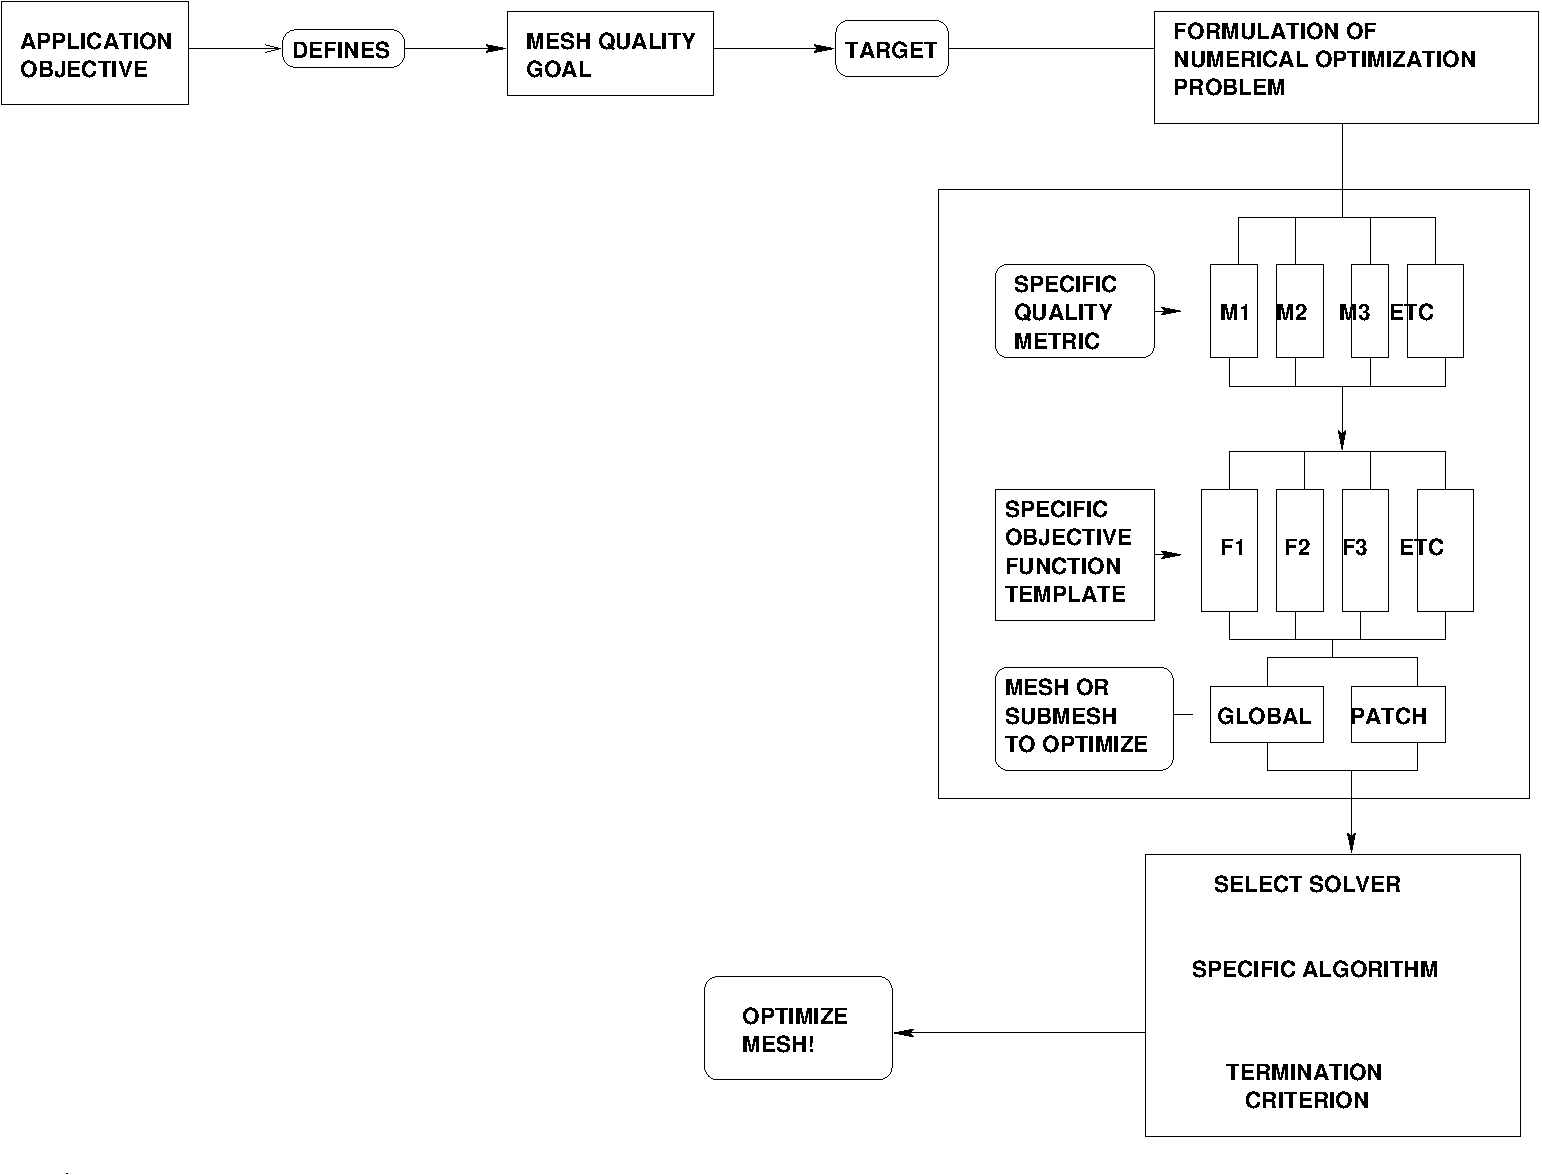
\includegraphics[width=4.7in]{figures/msq-paradigm}
\caption{\em The Mesquite Paradigm \label{Paradigm} }
%\end{tabular}
\end{center}
\end{figure}

\section{How to use this User's Manual}
This user's manual
\begin{itemize}
\item provides an introduction to mesh quality and basic Mesquite concepts (Chapter \ref{sec:intro}),
\item instructs novice users on how to download and install Mesquite (Chapter \ref{sec:install}),
\item provides a tutorial on Mesquite's simplified user's interface and Mesquite's detailed API (Chapter \ref{sec:examples}).
\item describes how to load a mesh in Mesquite via files (Chapter \ref{sec:meshes}), and
%\item provides instructions on using the extensive TSTT interface or a Mesquite mesh specific mesh
%      interface to load a mesh {\it dynamicallu} in Mesquite (sections \ref{sec:msq_mesh}, \ref{sec:TSTT}), and
\item describes Mesquite interactions with domain geometry (Chapter \ref{sec:geom}), and
\item describes Mesquite Wrappers (Chapter \ref{sec:wrappers}),
%\item Exposes in details the concepts and the mechanisms of the advanced API (chapter \ref{sec:API}), and
%\item instructs the user on how to add their own instances of quality
%metrics, objective functions, and solvers (chapter \ref{sec:extensions})
\end{itemize}

Consult the doxygen documentation for the API reference as well as details on the software. There
are two sets of doxygen documentations available:
\begin{itemize}
\item The developer doxygen doc is located in mesquite/doc/developer/. From that directory, you
      must run 'doxygen Mesquite.dox'.
\item The user doxygen doc (API doc) is located in mesquite/doc/user/doxygen. From that directory, you
      must run 'doxygen Mesquite-user.dox'.
\end{itemize}
The doxygen command will generate two directories: an html directory containing the file
index.html that you can open with your web browser, and a latex directory containing a Makefile that
will generate a dvi file.

%\section{Related Documents}

%Documentation of the Mesquite API can be generated from comments in the Mesquite
%source code using the Doxygen utility
%(\url{http://www.stack.nl/~dimitri/doxygen/}).
%To generate HTML and LaTeX copies of this documentation, execute the command
%{\tt doxygen Mesquite-user.dox} in the {\tt doc/usr/doxygen} subdirectory
%of the Mesquite source.

%Further information and related documentation are available on the
%Mesquite home page, located at:
%\url{http://www.cs.sandia.gov/optimization/knupp/Mesquite.html}.


% Installing Mesquite
\input{install.tex}

% Examples
\chapter{Examples} \label{sec:examples}

\section{Short Tutorial}

In this section, we write a driver code which calls the Mesquite
library to improve the quality of a test mesh. This tutorial section
is aimed at giving the user a feel for Mesquite: \emph{this section is not
where to look for detailed information}. In particular, information
pertaining to loading a particular mesh format (see Chapter \ref{sec:meshes}),
interacting through a particular mesh interface (section \ref{sec:MeshData}),
and details of defining geometric domains (see Chapter \ref{sec:geom}) are not
given in this section.

First, we write a small program using Mesquite's simplified API, or
wrappers, to show the fastest way to deploy Mesquite functionality to
improve a mesh.  The wrapper concept, as well as details about the
different wrappers available, are described in section
\ref{sec:tutWrapper}.  Following this first example, we set up customized mesh
improvement tool using Mesquite's low-level API, the details of which
are described in section \ref{sec:tutDetailedAPI}.

\subsection{Tutorial File Template}
\label{sec:tutfile}

To create and link a driver code, the Mesquite library must be
installed per the instructions of section \ref{sec:compiling}.
The commands and file names specified in this section are relative
to the installed \texttt{testsuite/tutorial} directory.  It
is assumed that that is the working diretory.
This tutorial begins with the file \texttt{tutorial.cpp},
which contains the following template:
\begin{verbatim}
1.  #include "Mesquite_all_headers.hpp"
    #include <ostream>
2.  using namespace Mesquite;
    int main(int argc, char* argv[])
    {
3.    MsqError err;

      if (argc != 2) {
        std::cerr << "Expected mesh file names as single argument."
                  << std::endl;
        exit (EXIT_FAILURE);
      }

      // new code starts here
4.    //...

      return 0;
    }
\end{verbatim}
The lines labeled 1-3 highlight three basic aspects of using Mesquite;
\begin{enumerate}
\item For convenience, Mesquite provides the header file
\begin{center}
\texttt{include/Mesquite\_all\_headers.hpp}
\end{center} which includes all Mesquite
headers. Although this is the easiest way to handle the include directives,
it may slow down compilation of the application.
\item All Mesquite classes are part of the \texttt{Mesquite} namespace.

\item  The \texttt{MsqError} class defines an object type used to communicate
Mesquite errors to the application.  The calling application must pass
an instance of the \texttt{MsqError} class or an instance of a subclass of
\texttt{MsqError} to many Mesquite functions.  The state of the error object
may be checked by casting the instance ot a Boolean or using it in a
Boolean context.  The state is cleared by calling the \texttt{clear} method.
\item In the sections that follow, we guide the user through the steps
necessary to smooth a mesh using Mesquite.  All new lines of code to be
added to the template file start in this position and are added in the order
in which they are discussed.
\end{enumerate}

The code above takes a mesh file name as a command line argument and
performs no action. We can compile it in the
(\texttt{examples/}) directory with the command:

\begin{verbatim}
                        make -f tutorial.make
\end{verbatim}


\subsection{Loading a Test Mesh}
\label{sec:tutMesh}
Our next step is to load one of the test meshes distributed with
Mesquite.  These meshes are distributed in the VTK unstructured mesh
format, the details of which are given in \cite{VTKbook, VTKuml}. This
format was chosen because of its readability and ease of use.
In this tutorial we use
the simplest mechanism for loadling a mesh into Mesquite; different
options are described in Chapter \ref{sec:meshes}.  In particular, to
load a VTK test mesh in Mesquite, instantiate the Mesquite mesh
database object,
\texttt{MeshImpl}, and use the \texttt{read\_vtk} member function by
adding the following lines to the file template described in
\ref{sec:tutfile}.
\begin{verbatim}
  Mesquite::MeshImpl my_mesh;
  my_mesh.read_vtk(argv[1], err);
  if (err)
  {
    std::cout << err << std::endl;
    return 1;
  }
\end{verbatim}

If the mesh read in contains more than one type of element, Mesquite will automatically
handle the mixed elements with no additional effort required.

Mesquite also provides a function to write a mesh
file in VTK format, given a \texttt{MeshImpl} object:
\begin{verbatim}
  my_mesh.write_vtk("original_mesh.vtk",err);
\end{verbatim}

Mesquite deals automatically with all types of supported elements
(triangles, quadrilaterals, tetrahedra, hexahedra, wedges, and pyramids),
and also hybrid meshes consisting of mixed element types.
Some meshes require geometry information as well.  When improving a surface mesh, Mesquite must be provided information
about surface(s) the mesh is constrained to lie on and the association between
mesh entities and entities of the geometric domain (surfaces, curves, etc.)
Because Mesquite is inherently a 3D code, all 2D meshes must specify some
geometry constraints.  The details
for general geometric surfaces are explained in Chapter
\ref{sec:geom}. In this section,
we show how to define the geometry of a 2D planar mesh, specified by a
point $(x,y,z)$ and a normal. For example, the following defines an xy-plane
shifted five units in the z-direction:
\begin{verbatim}
  Vector3D normal(0,0,1);
  Vector3D point(0,0,5);
  PlanarDomain my_mesh_plane(normal, point);
\end{verbatim}


\subsection{Improving the Mesh with a Wrapper Class}
\label{sec:tutWrapper}
The simplest way to use a Mesquite mesh quality improvement
procedure is to instantiate one of the wrapper classes described in Chapter
\ref{sec:wrappers}. Here, we will instantiate the
\texttt{LaplacianSmoother} wrapper and use it to improve
the Mesh we created earlier.  Mesquite can optimize the mesh
without further input from the user by utilizing preset, default
values.  If some customization is desired, the wrapper classes also
allow users to set the most important parameters of the underlying
algorithms and metrics (see Chapter
\ref{sec:wrappers} for details).
\begin{verbatim}
Mesquite::LaplaceWrapper mesh_quality_algorithm;

MeshDomainAssoc mesh_and_domain = MeshDomainAssoc(&my_mesh, &my_mesh_plane);
mesh_quality_algorithm.run_instructions(&mesh_and_domain, err);

//Should check the error object after the instruction is ran
// to see whether the instructions were all successful.
if (err)
{
    std::cout << err << std::endl;
    return 1;
}
\end{verbatim}

Once the algorithm has been executed using the {\tt run\_instructions} member
function of the wrapper class, the improved mesh can be written to a new
file:
\begin{verbatim}
  my_mesh.write_vtk("smoothed_mesh.vtk",err);
\end{verbatim}
This completes the code necessary for the simple wrapper example. Once
the code has successfully compiled by typing the {\tt make} command given in
section \ref{sec:tutfile},
run it from the tutorial directory \texttt{mesquite/testSuite/tutorial/}
with a mesh file name as a command line
argument by typing:
\begin{verbatim}
./tutorial ../../meshFiles/2D/quads/untangled/square_quad_10_rand.vtk
\end{verbatim}
The code creates the files original\_mesh.vtk
and improved\_mesh.vtk in the current directory.  These two meshes, the
original and the optimized, are
shown in figure \ref{fig:square_rand}.  The text output of the code,
shown below, reports the inverse mean ratio quality metric statistics for
the orginal mesh before optimization and the final mesh after optimization.
The optimized mesh consists
of square quadrilaterals which have an inverse mean ratio value of 1.0.
\begin{verbatim}
************** QualityAssessor(free only) Summary **************

  Evaluating quality for 100 elements.
  This mesh had 100 quadrilateral elements.
  There were no inverted elements detected.
  No entities had undefined values for any computed metric.

     Element Quality Statistics

     minimum     average         rms     maximum     std.dev.
     1.01013     1.16655      1.1738     1.79134     0.130322

     Number of statistics = 100
     Metric = Inverse Mean Ratio
     Element Quality not based on sample points.


************** QualityAssessor(free only) Summary **************

  Evaluating quality for 100 elements.
  This mesh had 100 quadrilateral elements.
  There were no inverted elements detected.
  No entities had undefined values for any computed metric.

     Element Quality Statistics

     minimum     average         rms     maximum     std.dev.
           1           1           1     1.00001 2.20663e-006

     Number of statistics = 100
     Metric = Inverse Mean Ratio
     Element Quality not based on sample points.
\end{verbatim}
\begin{figure*}[htbp]
\begin{center}
    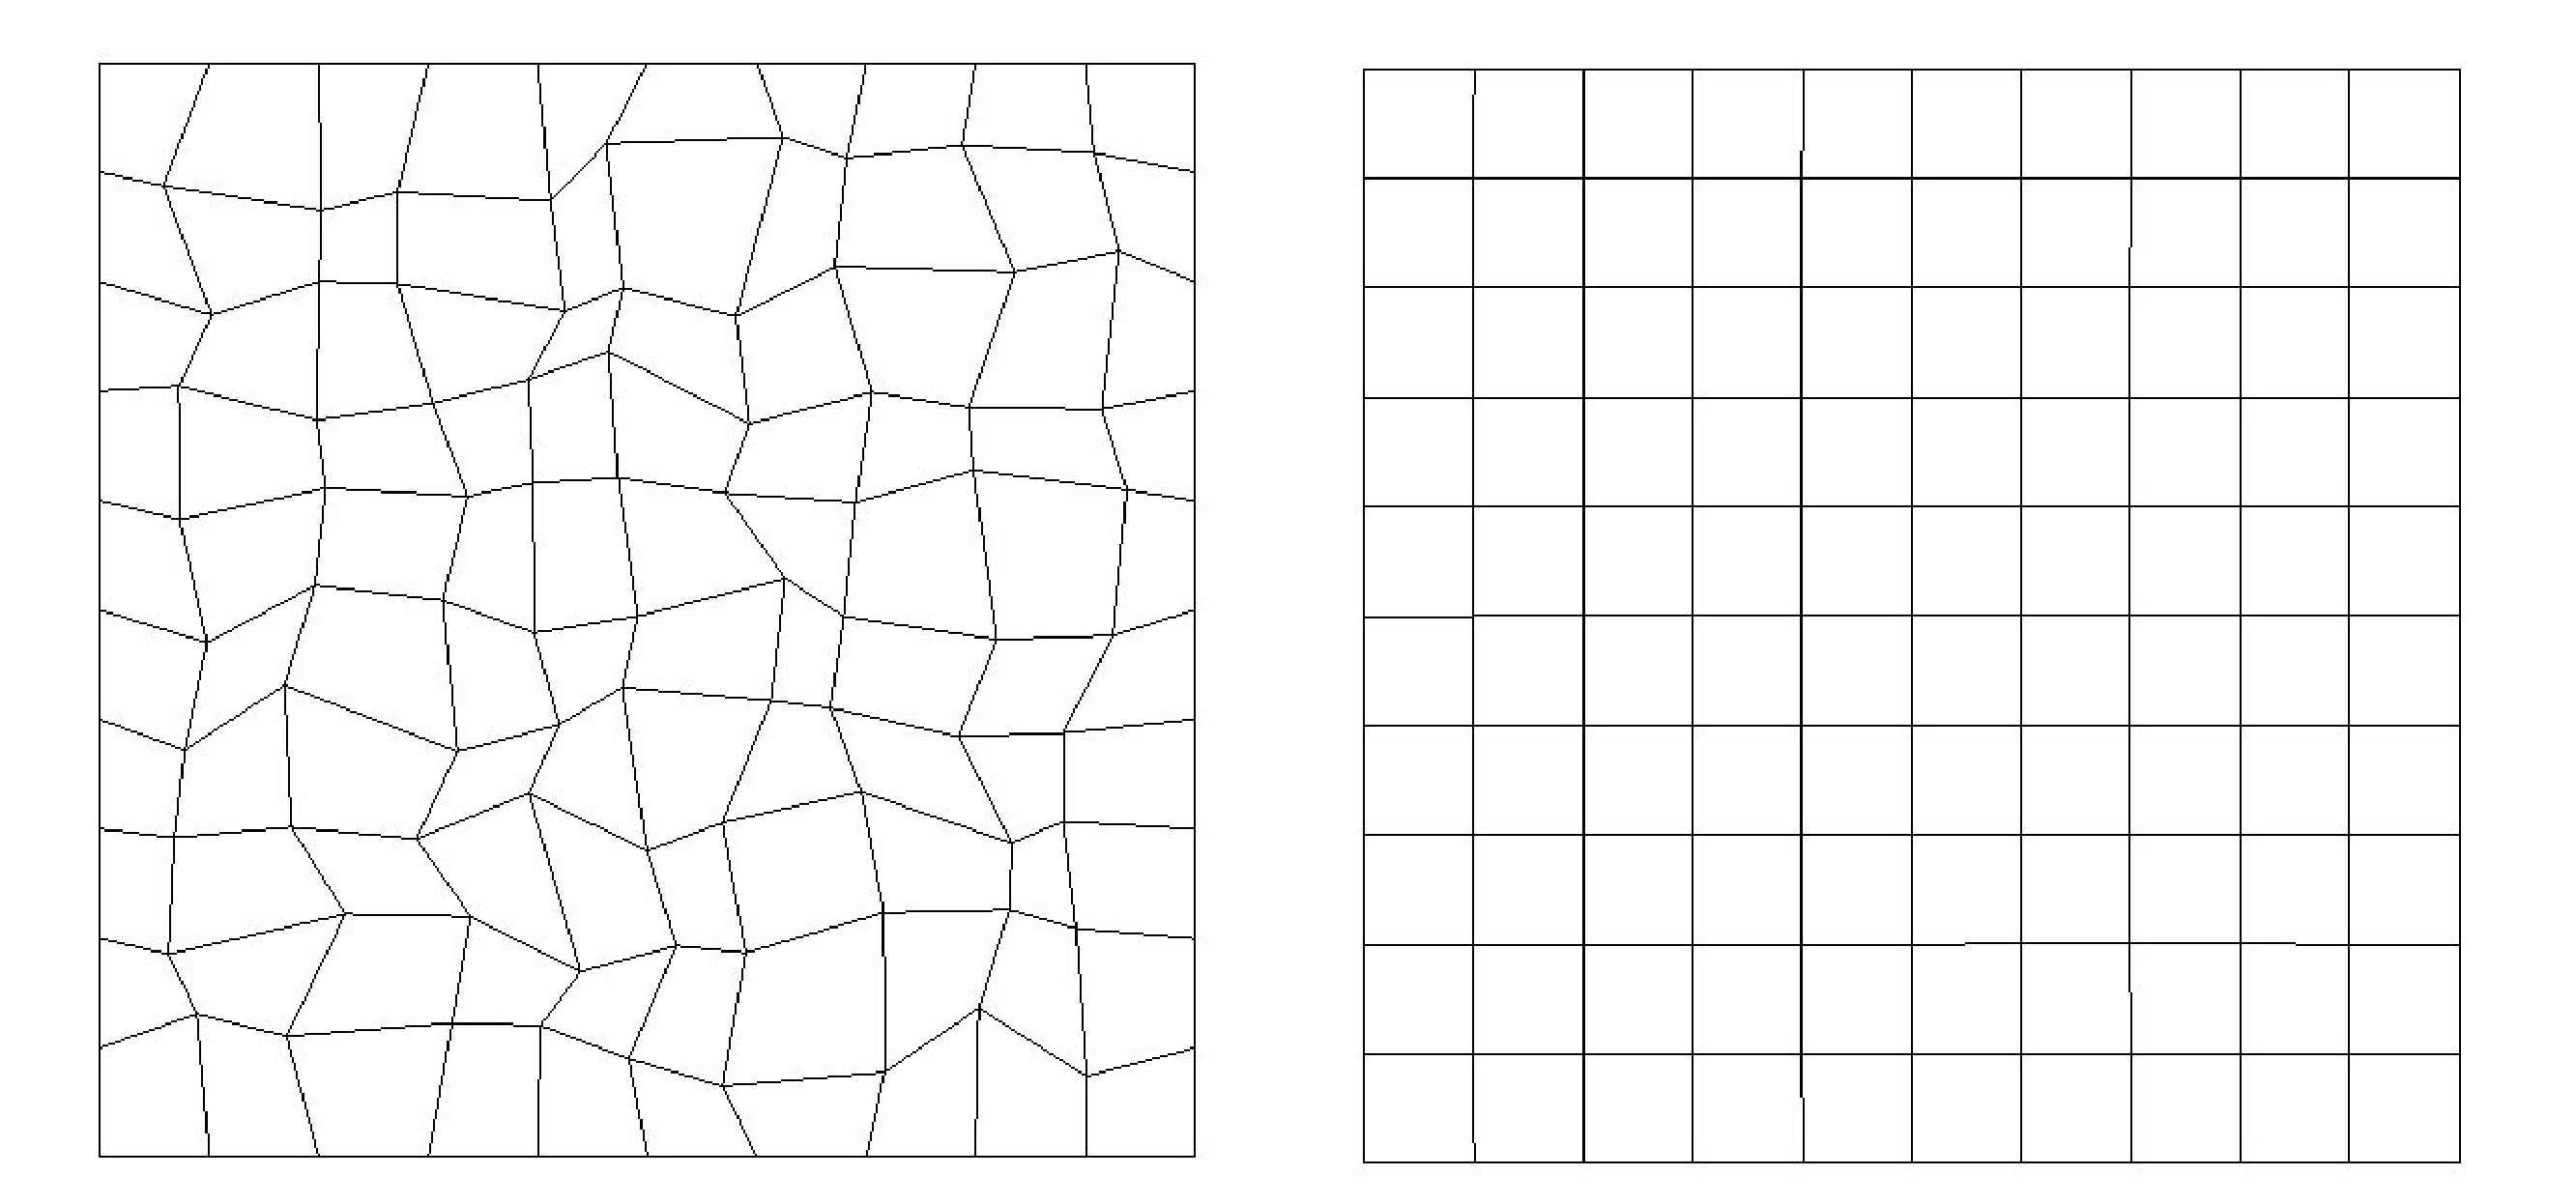
\includegraphics[height=80mm]{figures/square_rand}
    \caption{square\_quad\_10\_rand.vtk mesh. The original mesh is on the left, the mesh smoothed with the \texttt{LaplacianSmoother} is shown on the right.}
    \label{fig:square_rand}
\end{center}
\end{figure*}


\subsection{Improving the Mesh with the Low Level API}
\label{sec:tutDetailedAPI}
If the user requires in-depth control over the mesh quality improvement
process, the use of lower-level Mesquite classes provides an extensive
amount of flexibility.   In particular, the user can specify the quality
metric, objective function template, and optimization algorithm by
instantiating particular instances of each.  For each, various options
such as numerical or analytical gradient and Hessian evaluations or
the patch size can be selected.  Furthermore, the user can fine tune
the optimization algorithm performance by creating and setting the parameters
of the termination criteria.
%for both inner and outer iterations.
%mbrewer removed reference to inner and outer iterations.
%{\tt LAF have we talked about inner and outer iterations before? perhaps
%too advanced for the tutorial}

Once these core objects have been created and customized, the user
creates an instruction queue and adds one or more quality improvers
and quality assessors to it.  The mesh optimization process is initiated
with the {\tt run\_instructions} method on the instruction queue
class.

In this section, we provide a simple example to highlight the main
steps needed for this approach.  The code segment given below performs
the same functionality as the wrapper class highlighted in the
previous section.  The comment lines provide high level documentation;
the details of each class and the low-level API are not described here.
%extensively treated in Section
%\ref{sec:detailedAPI}.

\begin{verbatim}
    // creates a mean ratio quality metric ...
  IdealWeightInverseMeanRatio inverse_mean_ratio(err);

    // sets the objective function template
  LPtoPTemplate obj_func(&inverse_mean_ratio, 2, err);

    // creates the optimization procedures
  TrustRegion t_region(&obj_func);

    //performs optimization globally
  t_region.use_global_patch();

    // creates a termination criterion and
    // add it to the optimization procedure
    // outer loop: default behavior: 1 iteration
    // inner loop: stop if gradient norm < eps
  TerminationCriterion tc_inner;
  tc_inner.add_absolute_gradient_L2_norm( 1e-4 );
  t_region.set_inner_termination_criterion(&tc_inner);

    // creates a quality assessor
  QualityAssessor m_ratio_qa(&inverse_mean_ratio);
    // creates an instruction queue
  InstructionQueue queue;
  queue.add_quality_assessor(&m_ratio_qa, err);
  queue.set_master_quality_improver(&t_region, err);
  queue.add_quality_assessor(&m_ratio_qa, err);

    // do optimization of the mesh_set
  MeshDomainAssoc mesh_and_domain = MeshDomainAssoc(&my_mesh, &my_mesh_plane);
  queue.run_instructions(&mesh_and_domain, err);
  if (err) {
    std::cout << err << std::endl;
    return 2;
  }
\end{verbatim}

\newpage

\subsection{Mesh Improvement Examples}

The left image in figure \ref{fig:hole} shows a mesh that has
been degraded by moving the disk from the right side of the square to
the left while keeping the mesh topology fixed.
The mesh file
\newline
\texttt{mesquite/meshFiles/2D/vtk/quads/tangled/hole\_in\_square.vtk} contains the
information for this mesh.  If you plan to run this example, note that
the normal direction that defines the geometry is now $(0,0,-1)$.
This change must be made in the tutorial example code
as was done in section \ref{sec:tutMesh}, or an error message will be
thrown.
\begin{verbatim}
  Vector3D normal(0,0,-1);
  Vector3D point(0,0,-5);
  PlanarDomain my_mesh_plane(normal, point);
\end{verbatim}

We can now improve the mesh with the wrapper mentioned in
\ref{sec:tutWrapper} or the detailed API mentioned in
\ref{sec:tutDetailedAPI}.
Because we changed the normal, the driver code must be recompiled;
otherwise the code and executable are as before.
Once the code is recompiled, type
\begin{verbatim}
./tutorial ../../meshFiles/2D/vtk/quads/tangled/hole_in_square.vtk
\end{verbatim}
to improve this mesh.
The smoothed mesh is shown in the right image of figure
\ref{fig:hole}.
The vertex locations have been repositioned and significantly improve
the quality of the mesh, as shown by the onscreen
quality assessor output:
\begin{verbatim}
************** QualityAssessor(free only) Summary **************

  Evaluating quality for 140 elements.
  This mesh had 140 quadrilateral elements.
  There were no inverted elements detected.
  No entities had undefined values for any computed metric.

     Element Quality Statistics

     minimum     average         rms     maximum    std.dev.
     1.07588     85.8391     463.357     5037.46     455.336

     Number of statistics = 140
     Metric = Inverse Mean Ratio
     Element Quality not based on sample points.


************** QualityAssessor(free only) Summary **************

  Evaluating quality for 140 elements.
  This mesh had 140 quadrilateral elements.
  There were no inverted elements detected.
  No entities had undefined values for any computed metric.

     Element Quality Statistics

     minimum     average         rms     maximum    std.dev.
     1.01896     1.83479     1.91775     3.36336    0.557969

     Number of statistics = 140
     Metric = Inverse Mean Ratio
     Element Quality not based on sample points
\end{verbatim}
\begin{figure*}[htbp]
\begin{center}
    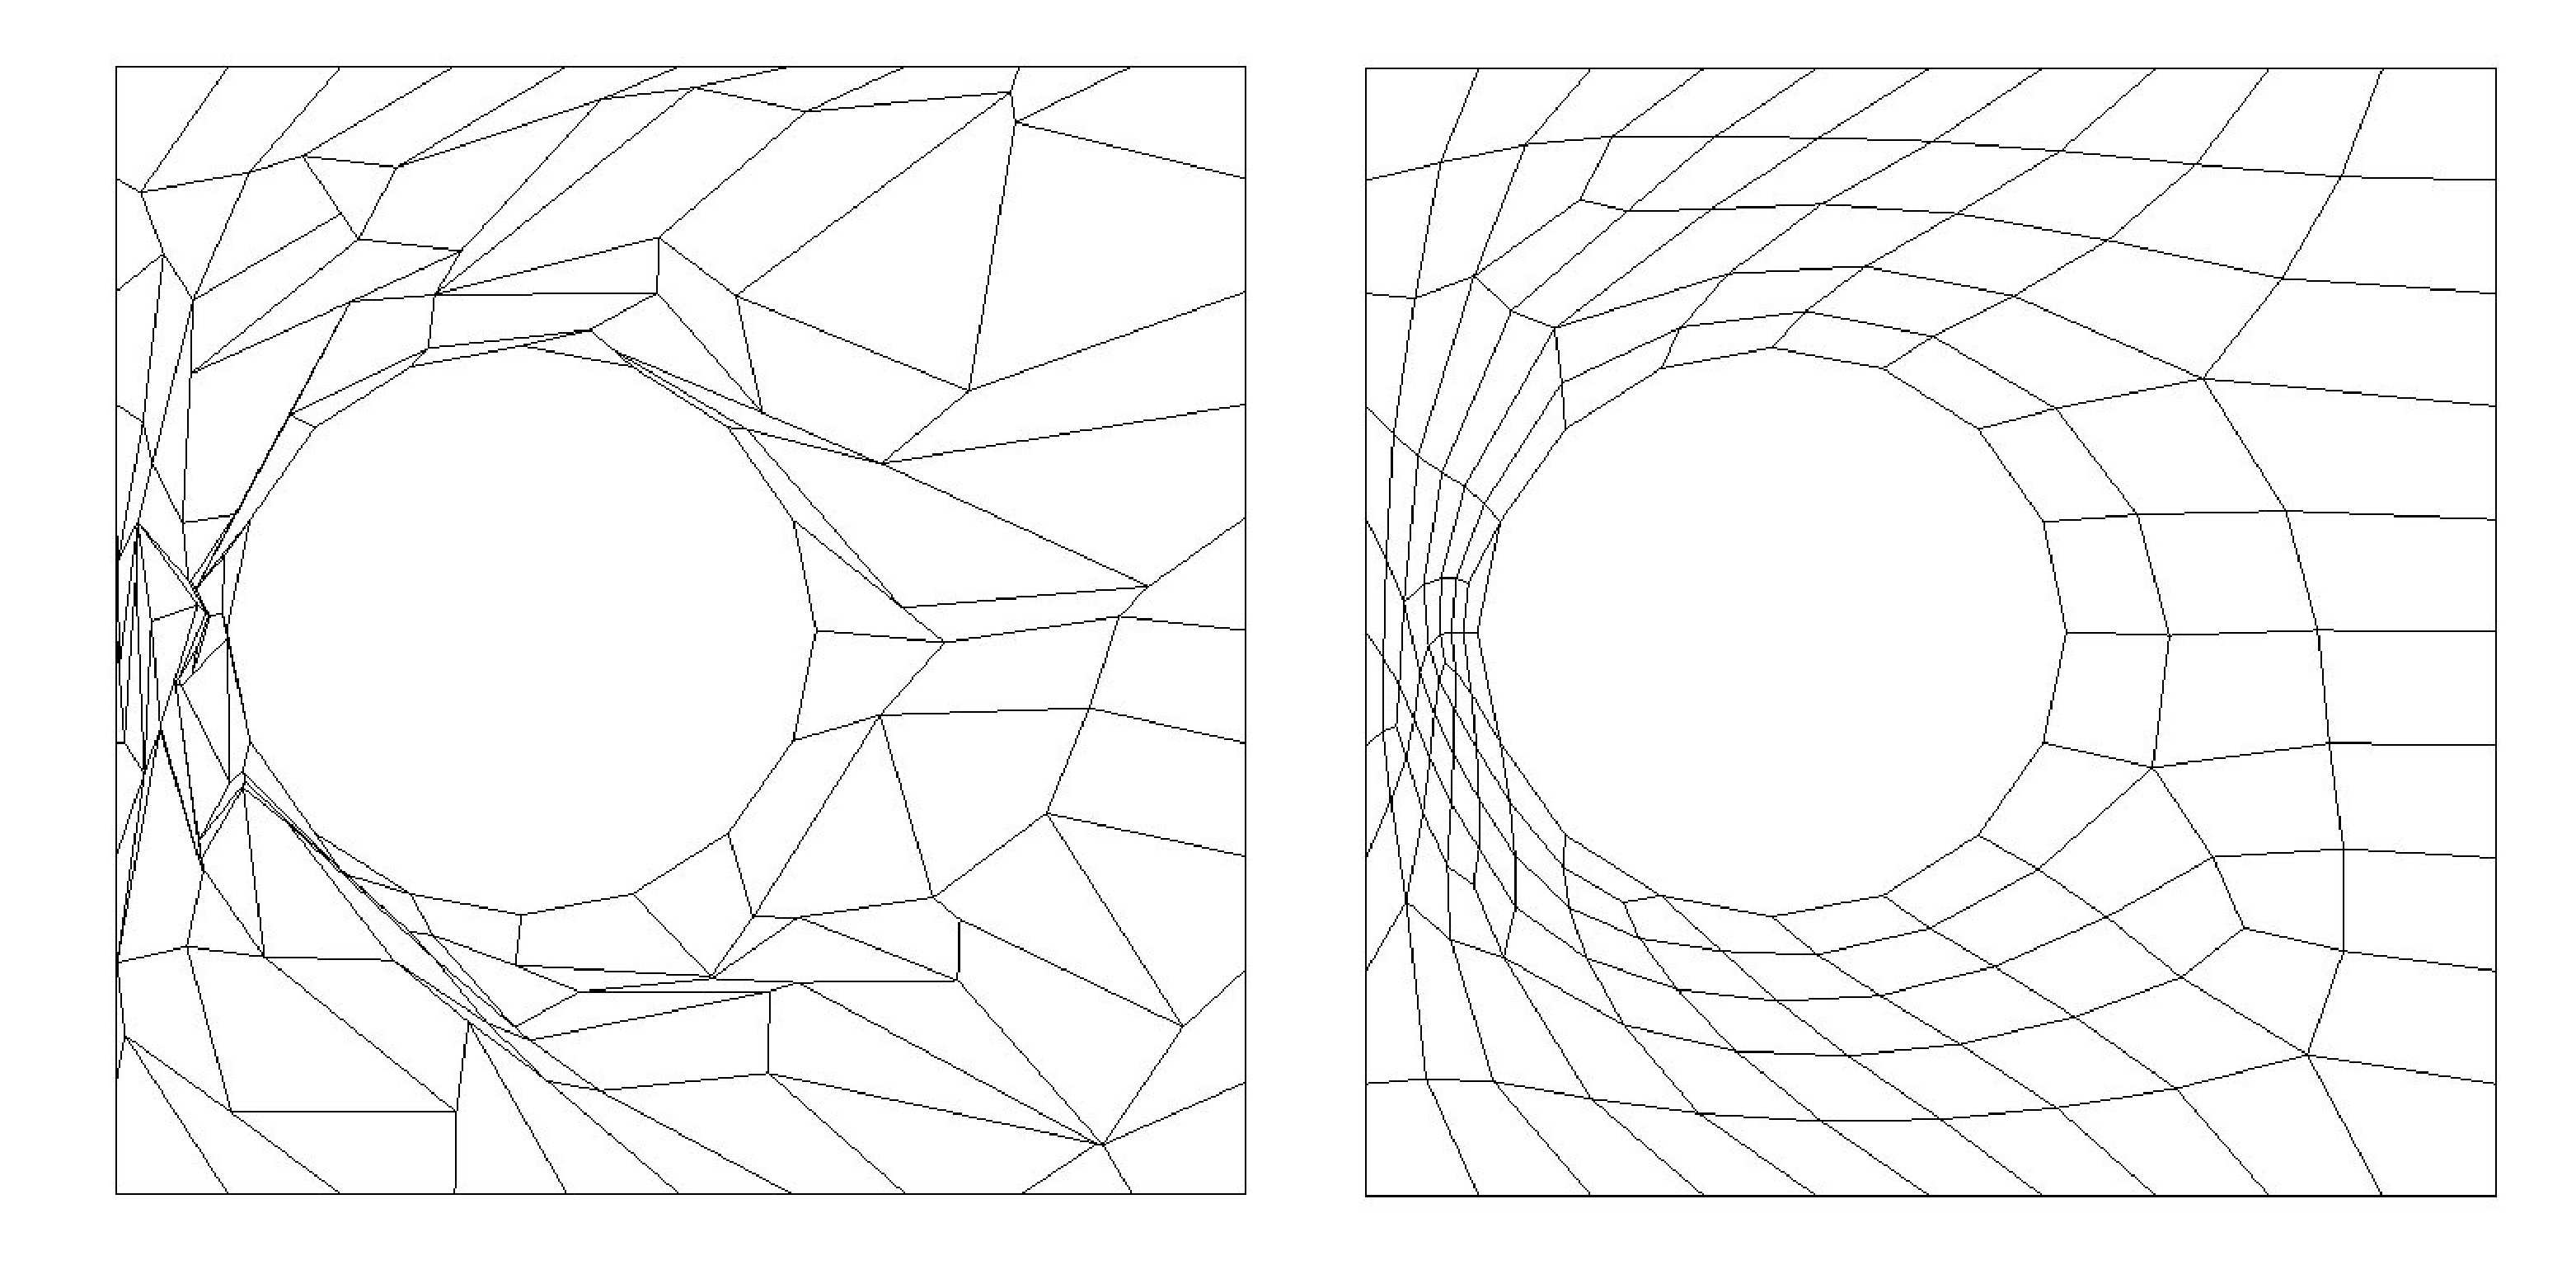
\includegraphics[height=80mm]{figures/hole_in_square}
    \caption{hole\_in\_square.vtk mesh. The original mesh is on the left, the mesh smoothed with
    Mesquite is shown on the right.}
    \label{fig:hole}
\end{center}
\end{figure*}


%%... section on testing ...

\subsection{Regression Testing}
\label{sec:RegressionTesting}
Regression testing encompasses
running unit tests as well as comparing results data against "blessed"
or "gold" data.  An example of comparing results of a smoothed mesh
against a gold version is in
\texttt{mesquite/testSuite/parallel\_smooth\_laplace/par\_hex\_smooth\_laplace.cpp}.
This utilizes a function in \texttt{MeshUtil}, \texttt{meshes\_are\_different}, to compare
two \texttt{MeshImpl} objects (within a specified numerical tolerance).  It is
recommended that both unit testing and gold-comparison testing be
included in your test code development.


% Getting Mesh Into Mesqite
\input{data.tex}

% Mesquite Features
\input{features.tex}

% Constraining Mesh to a Geometric Domain
\input{geom.tex}

% Mesquite Wrapper Descriptions
\chapter{Mesquite Wrapper Descriptions}
\label{sec:wrappers}

Applications which desire to access Mesquite capabilities without delving
into the low-level API can invoke wrappers to perform basic mesh quality
improvement tasks that, except for a few user-defined inputs, are fully
automatic. The wrappers target classic mesh optimization problems that occur
repeatedly across many applications. See section 3.1.3 for an example of how
to invoke a wrapper.
This chapter provides a summary of the current Mesquite wrappers. \newline

\noindent Note that the wrappers do not, by themselves, completely define
the optimization problem.  The user still has to set the fixed/free flags,
and the values of the termination criteria.  \newline

\section{Laplace-smoothing} \label{sec:LaplaceWrapper}

\noindent {\it Name}: LaplaceWrapper \newline
\noindent {\it Purpose}: Produce a {\it smooth} mesh. \newline
\noindent {\it Notes}: This is a local patch relaxation-solver. A 'smart'
Laplacian solver is also available in Mesquite, but it is not used in this
wrapper.  \newline
\noindent {\it Limitations/assumptions}: No invertibility guarantee. \newline
\noindent {\it Input Termination Criterion}: Stop after 10 global iterations. \newline \newline

\noindent Under the Cover: \newline
\noindent {\it Hardwired Parameters}: None \newline
\noindent {\it Mesh/Element Type}: Any supported type. \newline
\noindent {\it Global/Local}: Local Patch with Culling \newline

\noindent Example: \newline

\begin{verbatim}
************** QualityAssessor(free only) Summary **************

  Evaluating quality for 64 elements.
  This mesh had 64 quadrilateral elements.
  THERE ARE 28 INVERTED ELEMENTS.
  (Elements invalid at 108 of 256 sample locations.)

  28 OF 64 ENTITIES EVALUATED TO AN UNDEFINED VALUE FOR Inverse Mean Ratio

     Element Quality Statistics

     minimum     average         rms     maximum    std.dev.
           0     1.48854     2.00094     3.15625     1.33716

     Number of statistics = 64
     Metric = Inverse Mean Ratio
     Element Quality not based on sample points.


************** QualityAssessor(free only) Summary **************

  Evaluating quality for 64 elements.
  This mesh had 64 quadrilateral elements.
  There were no inverted elements detected.
  No entities had undefined values for any computed metric.

     Element Quality Statistics

     minimum     average         rms     maximum    std.dev.
           1           1           1           1           0

     Number of statistics = 64
     Metric = Inverse Mean Ratio
     Element Quality not based on sample points.
\end{verbatim}
\begin{figure*}[htbp]
\begin{center}
    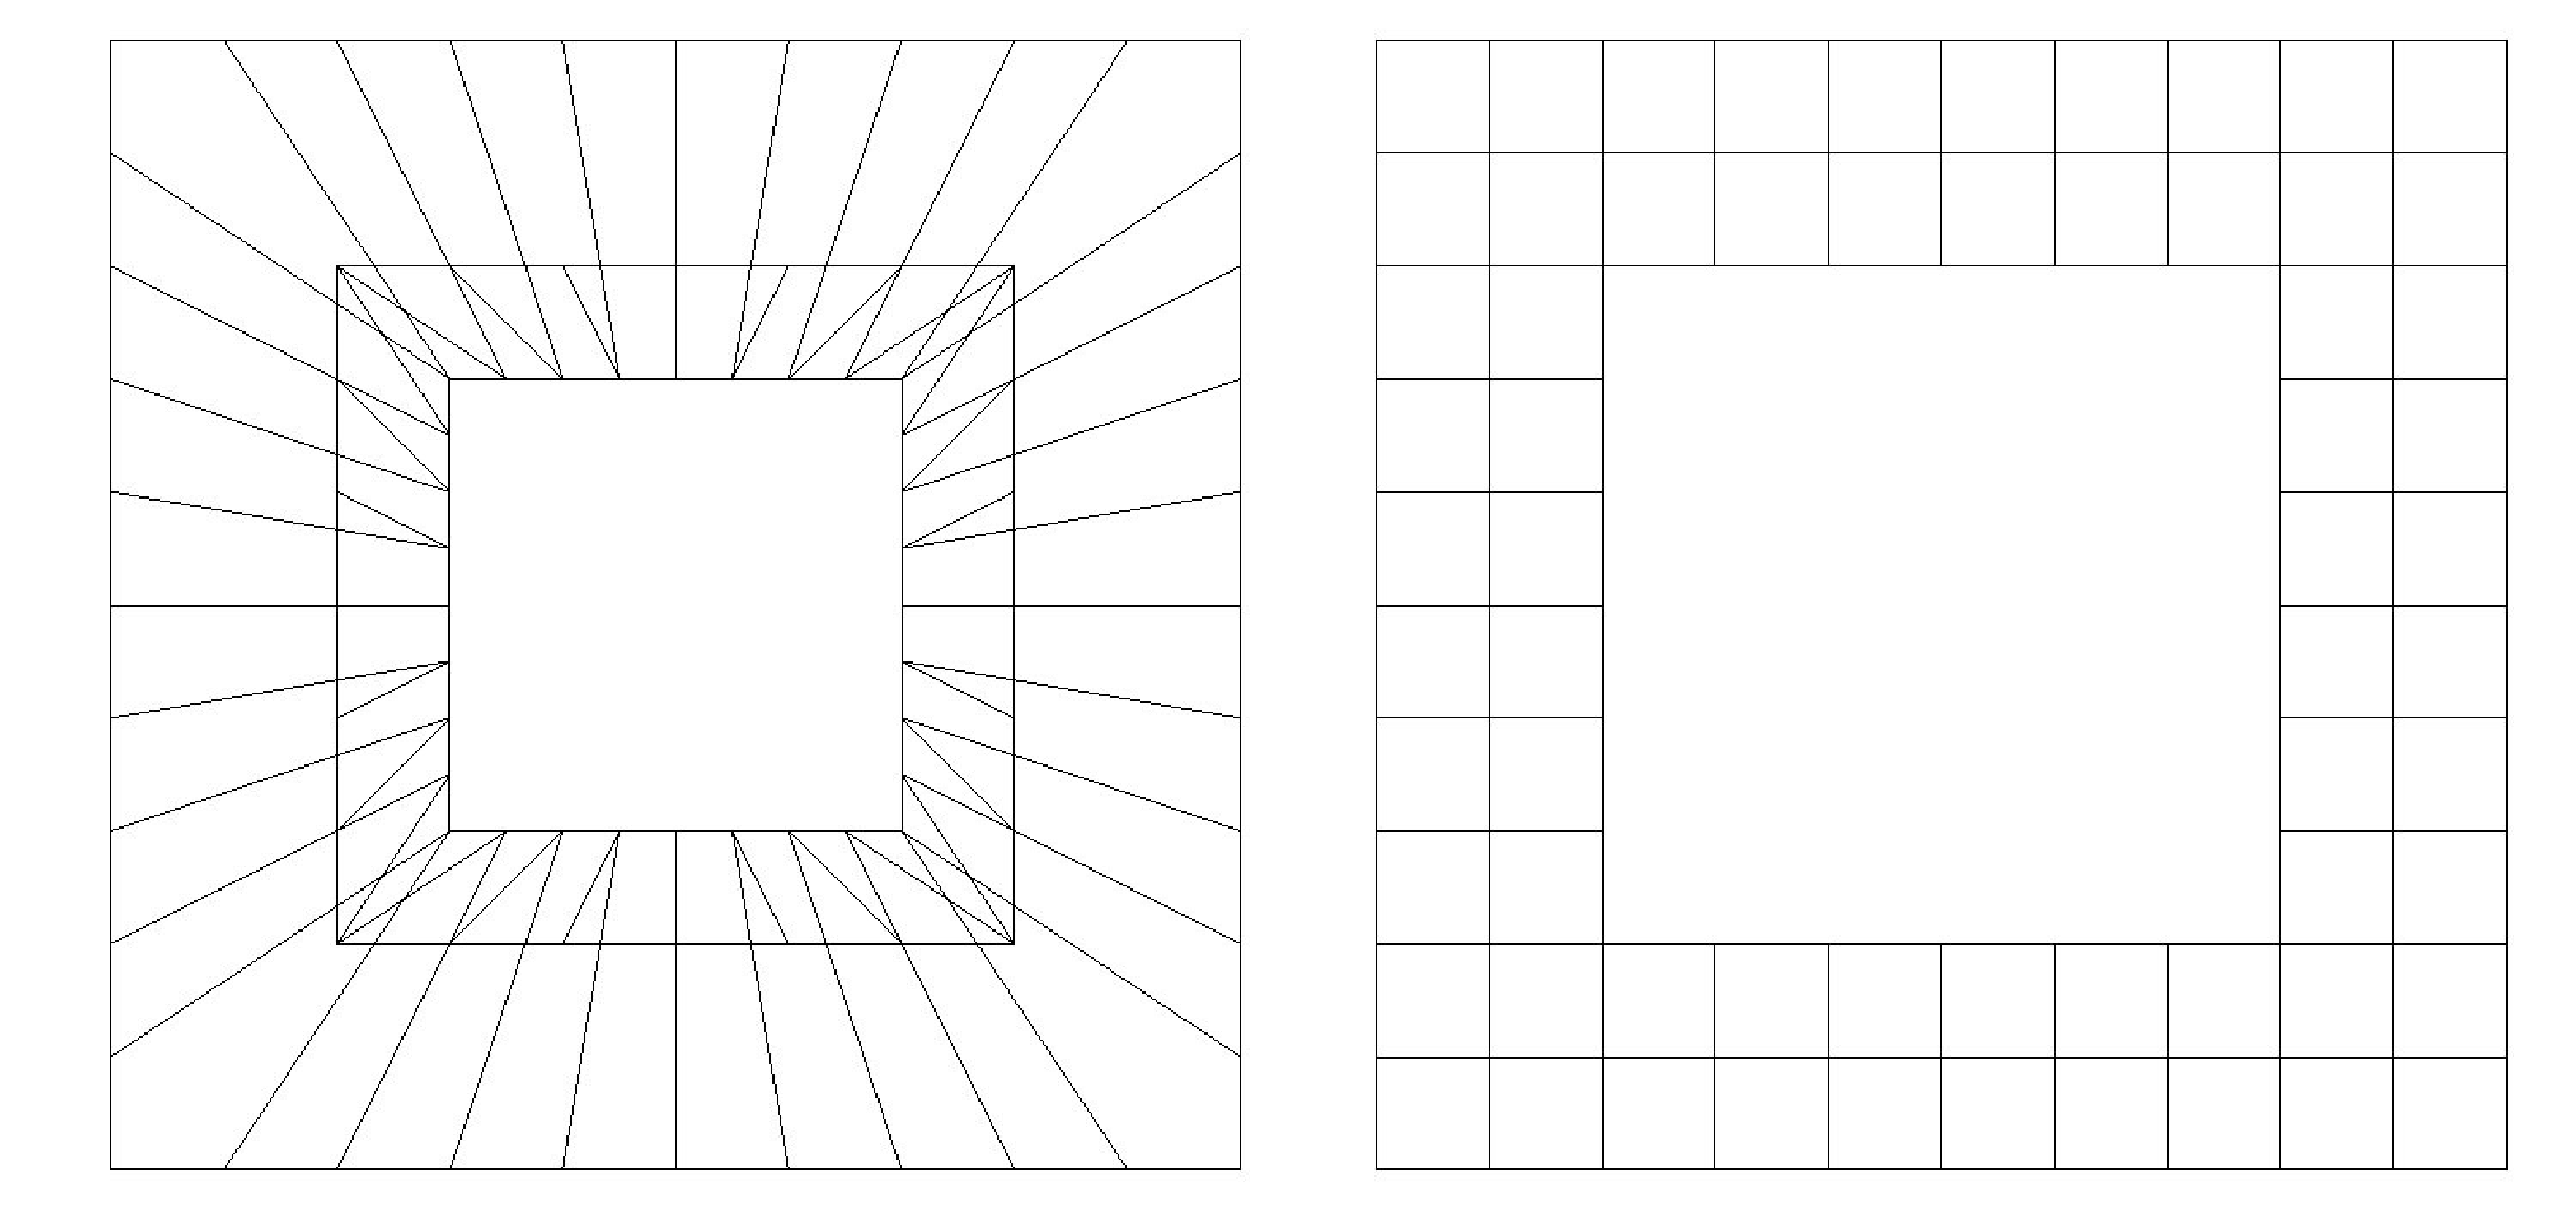
\includegraphics[height=75mm]{figures/inverted-hole-1}
    \caption{LaplaceWrapper, file: inverted-hole-1.vtk mesh. The original mesh is on the left, the mesh smoothed with the \texttt{LaplacianSmoother} is shown on the right.}
    \label{fig:inverted_hole_1}
\end{center}
\end{figure*}

\newpage

\section{Shape-Improvement} \label{sec:ShapeImprover}

\noindent {\it Name}: ShapeImprover \newline
\noindent {\it Purpose}: Make the shape of an element as close as possible to
that of the ideal/regular element shape. For example, make triangular and
tetrahedral elements equilateral.  The wrapper will use a non-barrier metric on meshes that contain inverted elements
and will use a barrier metric if the mesh does not contain inverted elements.  The default CPU time limit is 300 seconds.\newline
\noindent {\it Notes}: There is no guarantee that the wrapper will be able to successfully untangle a mesh that contains inverted elements.\newline
\noindent {\it Limitations/assumptions}:  \newline
\noindent {\it Input Termination Criterion}: CPU time limit of 300 seconds or maximum absolute vertex movement of 10 percent of the minimum edge length. \newline \newline

\noindent Under the Cover: \newline
\noindent {\it Metric}: TMPQualityMetric(Shape/ShapeBarrier) \newline
\noindent {\it Objective Function}: Algebraic mean of quality metric values \newline
\noindent {\it Mesh/Element Type}: Any supported type. \newline
\noindent {\it Solver}: Conjugate Gradient \newline
\noindent {\it Global/Local}: Global \newline

\noindent Example: \newline

\begin{verbatim}
************** QualityAssessor(free only) Summary **************

  Evaluating quality for 40 elements.
  This mesh had 40 quadrilateral elements.
  There were no inverted elements detected.
  No entities had undefined values for any computed metric.

     Element Quality Statistics

     minimum     average         rms     maximum    std.dev.
   0.0767863    0.232261    0.262717    0.404594    0.122781

     Number of statistics = 40
     Metric = ElementPMeanP(TShapeB1)
     Element Quality not based on sample points.


************** QualityAssessor(free only) Summary **************

  Evaluating quality for 40 elements.
  This mesh had 40 quadrilateral elements.
  There were no inverted elements detected.
  No entities had undefined values for any computed metric.

     Element Quality Statistics

     minimum     average         rms     maximum    std.dev.
    0.124926    0.204118    0.207417    0.328688   0.0368497

     Number of statistics = 40
     Metric = ElementPMeanP(TShapeB1)
     Element Quality not based on sample points.
\end{verbatim}

\begin{figure*}[htbp]
\begin{center}
    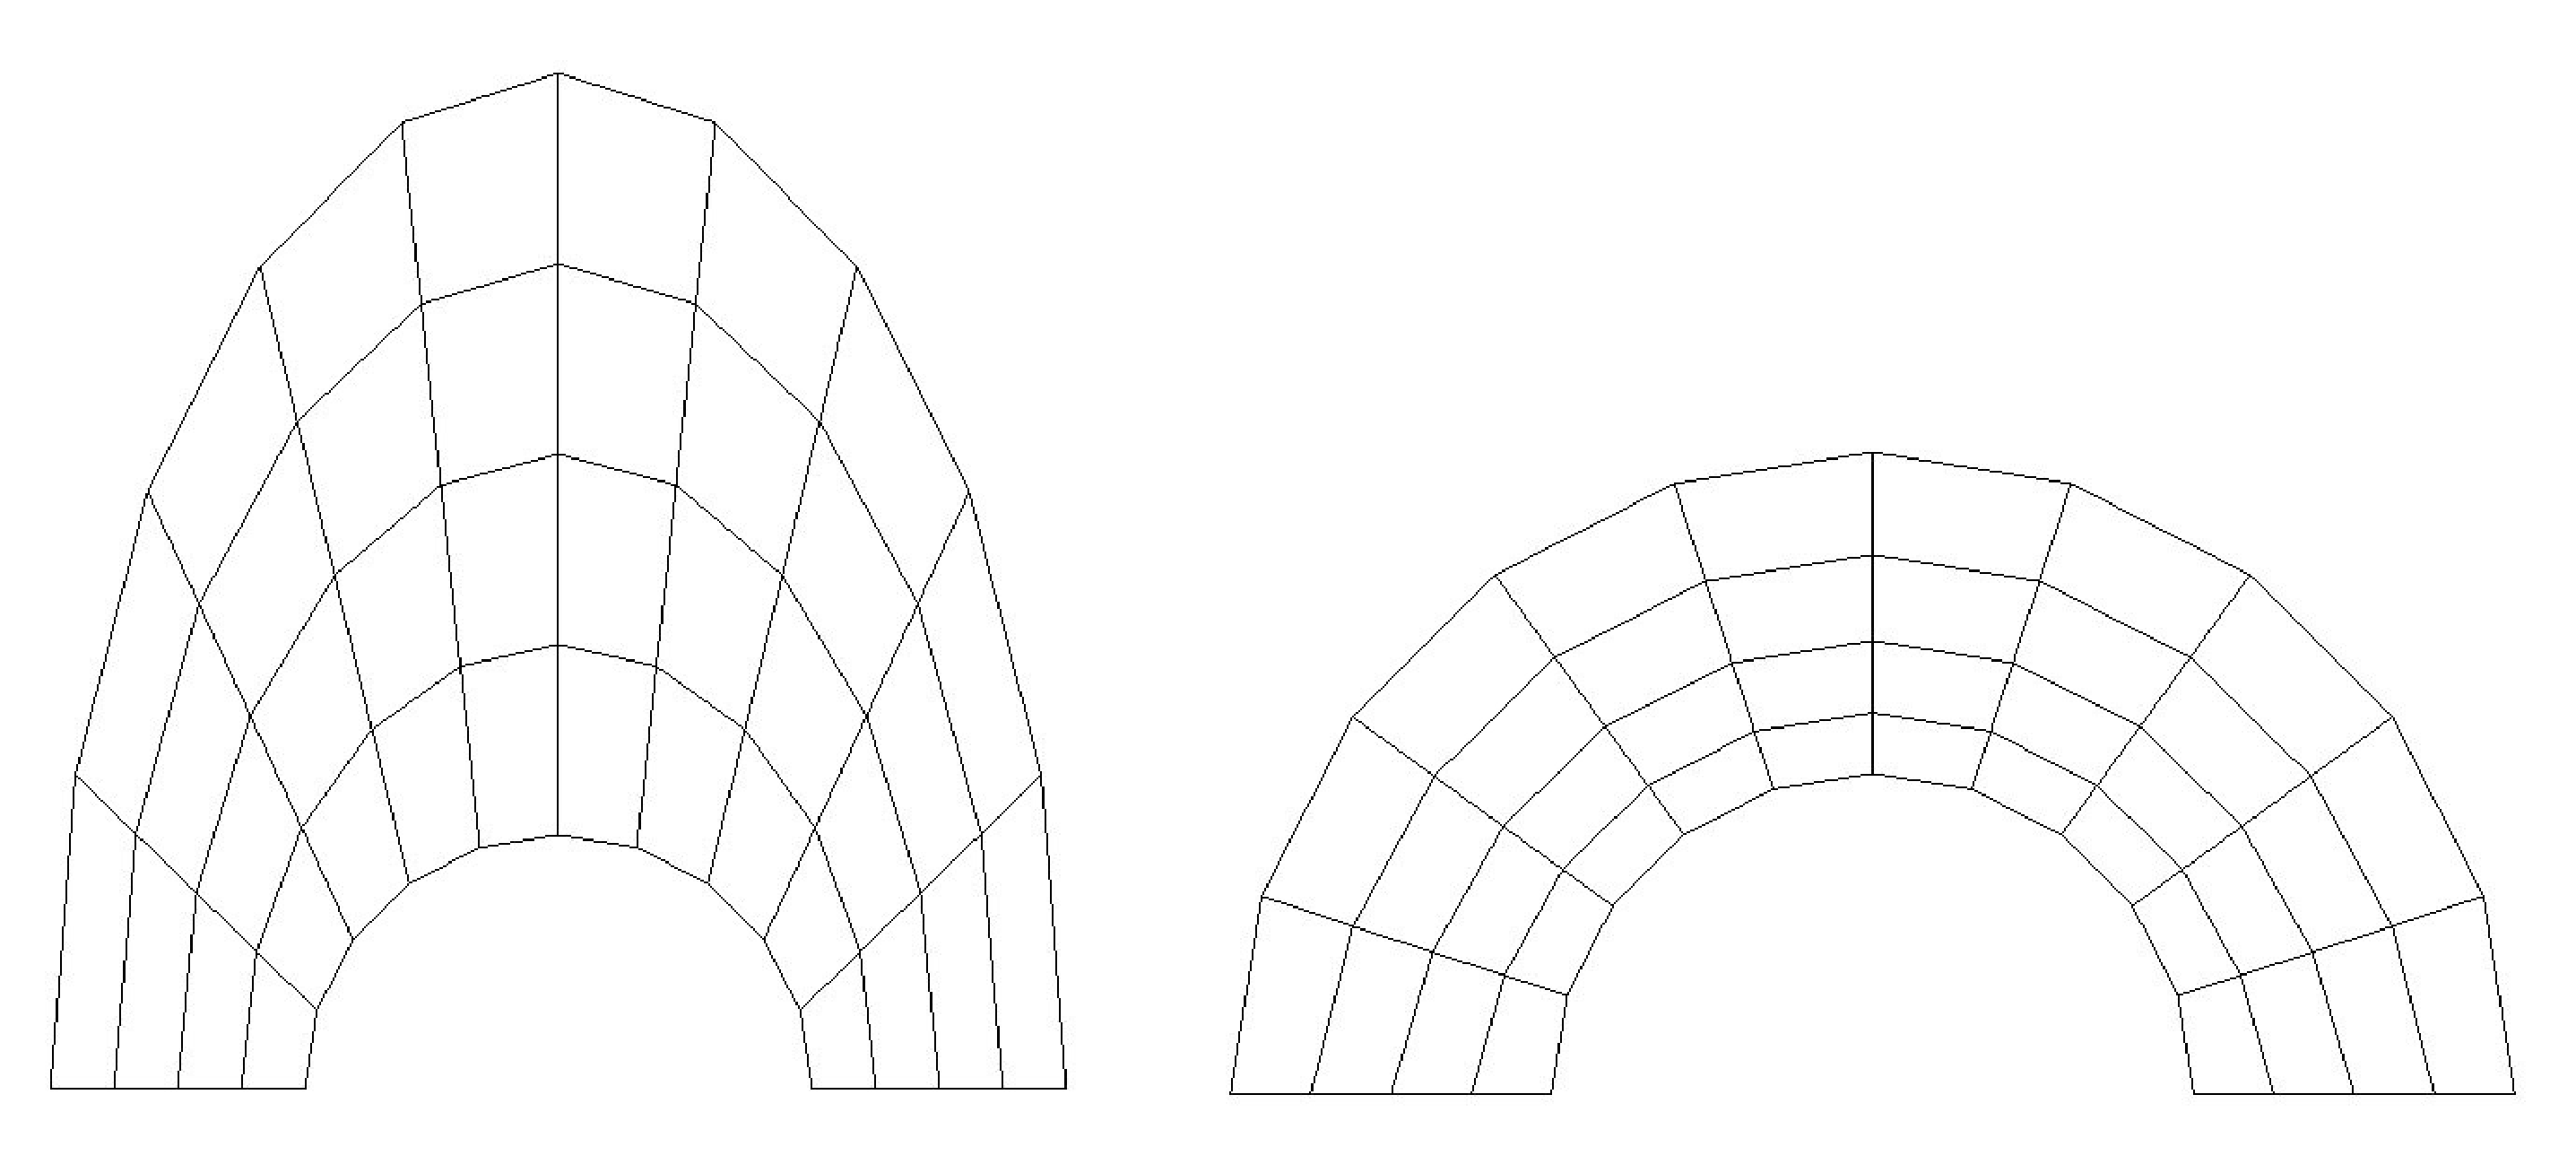
\includegraphics[height=80mm]{figures/horseshoe-10x4}
    \caption{ShapeImproverWrapper, file: tfi\_horse10x4-12.vtk mesh. The original mesh is on the left, the improved mesh is shown on the right.}
    \label{fig:inverted-hole-1}
\end{center}
\end{figure*}

\newpage

\section{Untangler} \label{sec:Untangler}

\noindent {\it Name}: UntangleWrapper \newline
\noindent {\it Purpose}: Untangle elements.  Prioritizes untangling over
element shape or other mesh quality measures.  \newline
\noindent {\it Notes}: A second optimization to improve element quality
after untangling is often necessary.  \newline
\noindent {\it Limitations/assumptions}: There is no guarantee that the optimal mesh computed using this wrapper will, in fact, be untangled.  \newline
\noindent {\it Input Termination Criterion}: CPU time limit (not used if input
value is non-positive) or fraction of mean edge length (default is 0.005).  It
also terminates if all elements are untangled, such that it should not modify
an input mesh with no inverted elements. \newline \newline

\noindent Under the Cover: \newline
\noindent {\it Metric}: TUntangleBeta or TUntangleMu(TSizeNB1) or TUntangleMu(TShapeSizeNB1) \newline
\noindent {\it Objective Function}: Algebraic mean of quality metric values \newline
\noindent {\it Mesh/Element Type}: Any supported type. \newline
\noindent {\it Solver}: Steepest Descent \newline
\noindent {\it Global/Local}: Local with culling, optionally Jacobi \newline

\noindent Example: \newline

\begin{verbatim}
************** QualityAssessor(free only) Summary **************

  Evaluating quality for 1024 elements.
  This mesh had 1024 quadrilateral elements.
  THERE ARE 9 INVERTED ELEMENTS.
  (Elements invalid at 9 of 4096 sample locations.)

  No entities had undefined values for any computed metric.

     Element Quality Statistics

     minimum     average         rms     maximum    std.dev.
           0     48.5379     210.965     2915.69     205.305

     Number of statistics = 1024
     Metric = ElementPMeanP(untangle(2D:TShapeSize2DNB1; 3D:TShapeSize3DNB1))
     Element Quality not based on sample points.

************** QualityAssessor(free only) Summary **************

  Evaluating quality for 1024 elements.
  This mesh had 1024 quadrilateral elements.
  There were no inverted elements detected.
  No entities had undefined values for any computed metric.

     Element Quality Statistics

     minimum     average         rms     maximum    std.dev.
           0     1.46636     23.8476     462.591     23.8025

     Number of statistics = 1024
     Metric = ElementPMeanP(untangle(2D:TShapeSize2DNB1; 3D:TShapeSize3DNB1))
     Element Quality not based on sample points.
\end{verbatim}


\begin{figure*}[htbp]
\begin{center}
    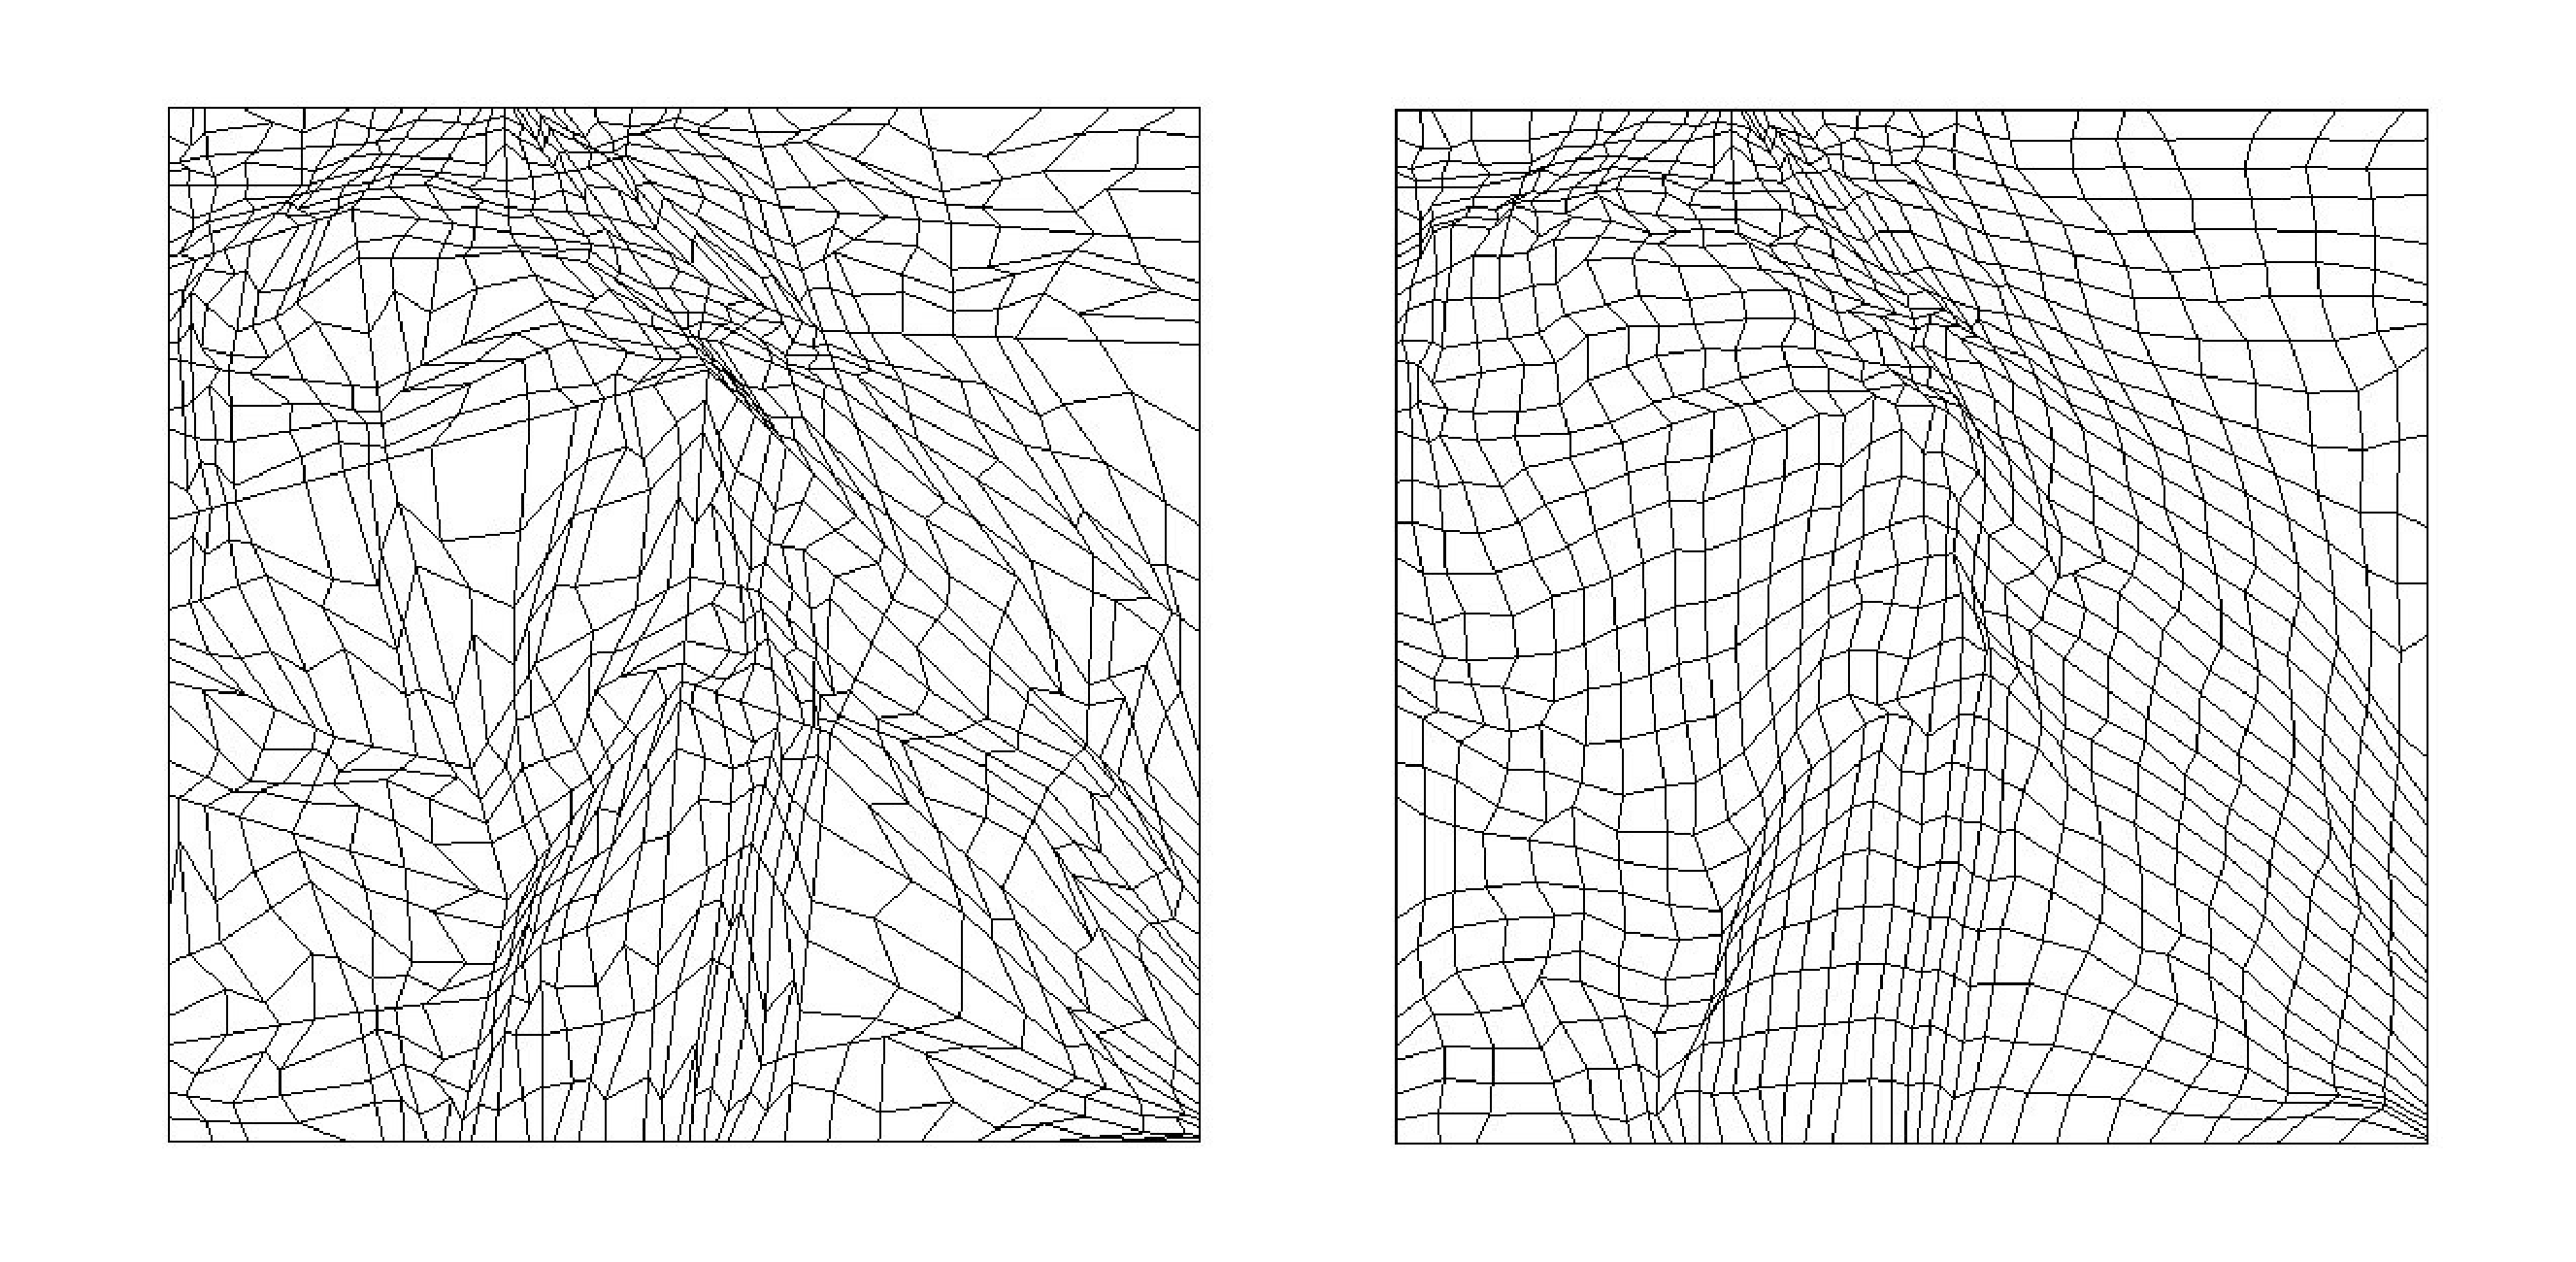
\includegraphics[height=80mm]{figures/shest_grid32}
    \caption{UntangleWrapper, TShapeSizeNB1 option, file: shest\_grid32.vtk mesh. The original mesh is on the left, the untangled mesh is shown on the right.}
    \label{fig:shest_grid32}
\end{center}
\end{figure*}

\newpage

\section{Minimum Edge-Length Improvement} \label{sec:PaverMinEdgeLengthWrapper}

\noindent {\it Name}: PaverMinEdgeLengthWrapper \newline
\noindent {\it Purpose}: Make all the edges in the mesh of equal length while
moving toward the ideal shape. Intended for explicit PDE codes whose
time-step limination is governed by the minimum edge-length in the mesh. \newline
\noindent {\it Notes}: Based on Target-matrix paradigm. \newline
\noindent {\it Limitations/assumptions}: Initial mesh must be non-inverted. User does not want to preserve or create anisotropic elements. \newline
\noindent {\it Input Termination Criterion}: maximum iterations (default=50), maximum absolute vertex movement \newline \newline

\noindent Under the Cover: \newline
\noindent {\it Hardwired Parameters}: None \newline
\noindent {\it Metric}:  Target2DShapeSizeBarrier or Target3DShapeSizeBarrier \newline
\noindent {\it Tradeoff Coefficient}: 1.0 \newline
\noindent {\it Objective Function}: Linear Average over the Sample Points \newline
\noindent {\it Mesh/Element Type}: Any supported type.  \newline
\noindent {\it Solver}: Trust Region \newline
\noindent {\it Global/Local}: Global \newline

\noindent Example: \newline

\begin{verbatim}
************** QualityAssessor(free only) Summary **************

  Evaluating quality for 8 elements.
  This mesh had 8 quadrilateral elements.
  There were no inverted elements detected.
  No entities had undefined values for any computed metric.

     Element Quality Statistics

     minimum     average         rms     maximum    std.dev.
    0.357275    0.983461     1.33806     3.27555    0.907303

     Number of statistics = 8
     Metric = ElementPMeanP(TShapeSizeB1)
     Element Quality not based on sample points.

    -------------------------------------------
     Element Quality Statistics

     minimum     average         rms     maximum    std.dev.
    0.538516     1.11317     1.15398     1.51327    0.304184

     Number of statistics = 12
     Metric = EdgeLength
     Element Quality not based on sample points.



************** QualityAssessor(free only) Summary **************

  Evaluating quality for 8 elements.
  This mesh had 8 quadrilateral elements.
  There were no inverted elements detected.
  No entities had undefined values for any computed metric.

     Element Quality Statistics

     minimum     average         rms     maximum    std.dev.
  0.00135009   0.0017804  0.00179488  0.00221721 0.000227498

     Number of statistics = 8
     Metric = ElementPMeanP(TShapeSizeB1)
     Element Quality not based on sample points.

    -------------------------------------------
     Element Quality Statistics

     minimum     average         rms     maximum    std.dev.
    0.994086      1.0004     1.00041     1.00293  0.00253389

     Number of statistics = 12
     Metric = EdgeLength
     Element Quality not based on sample points.
\end{verbatim}


\begin{figure*}[htbp]
\begin{center}
    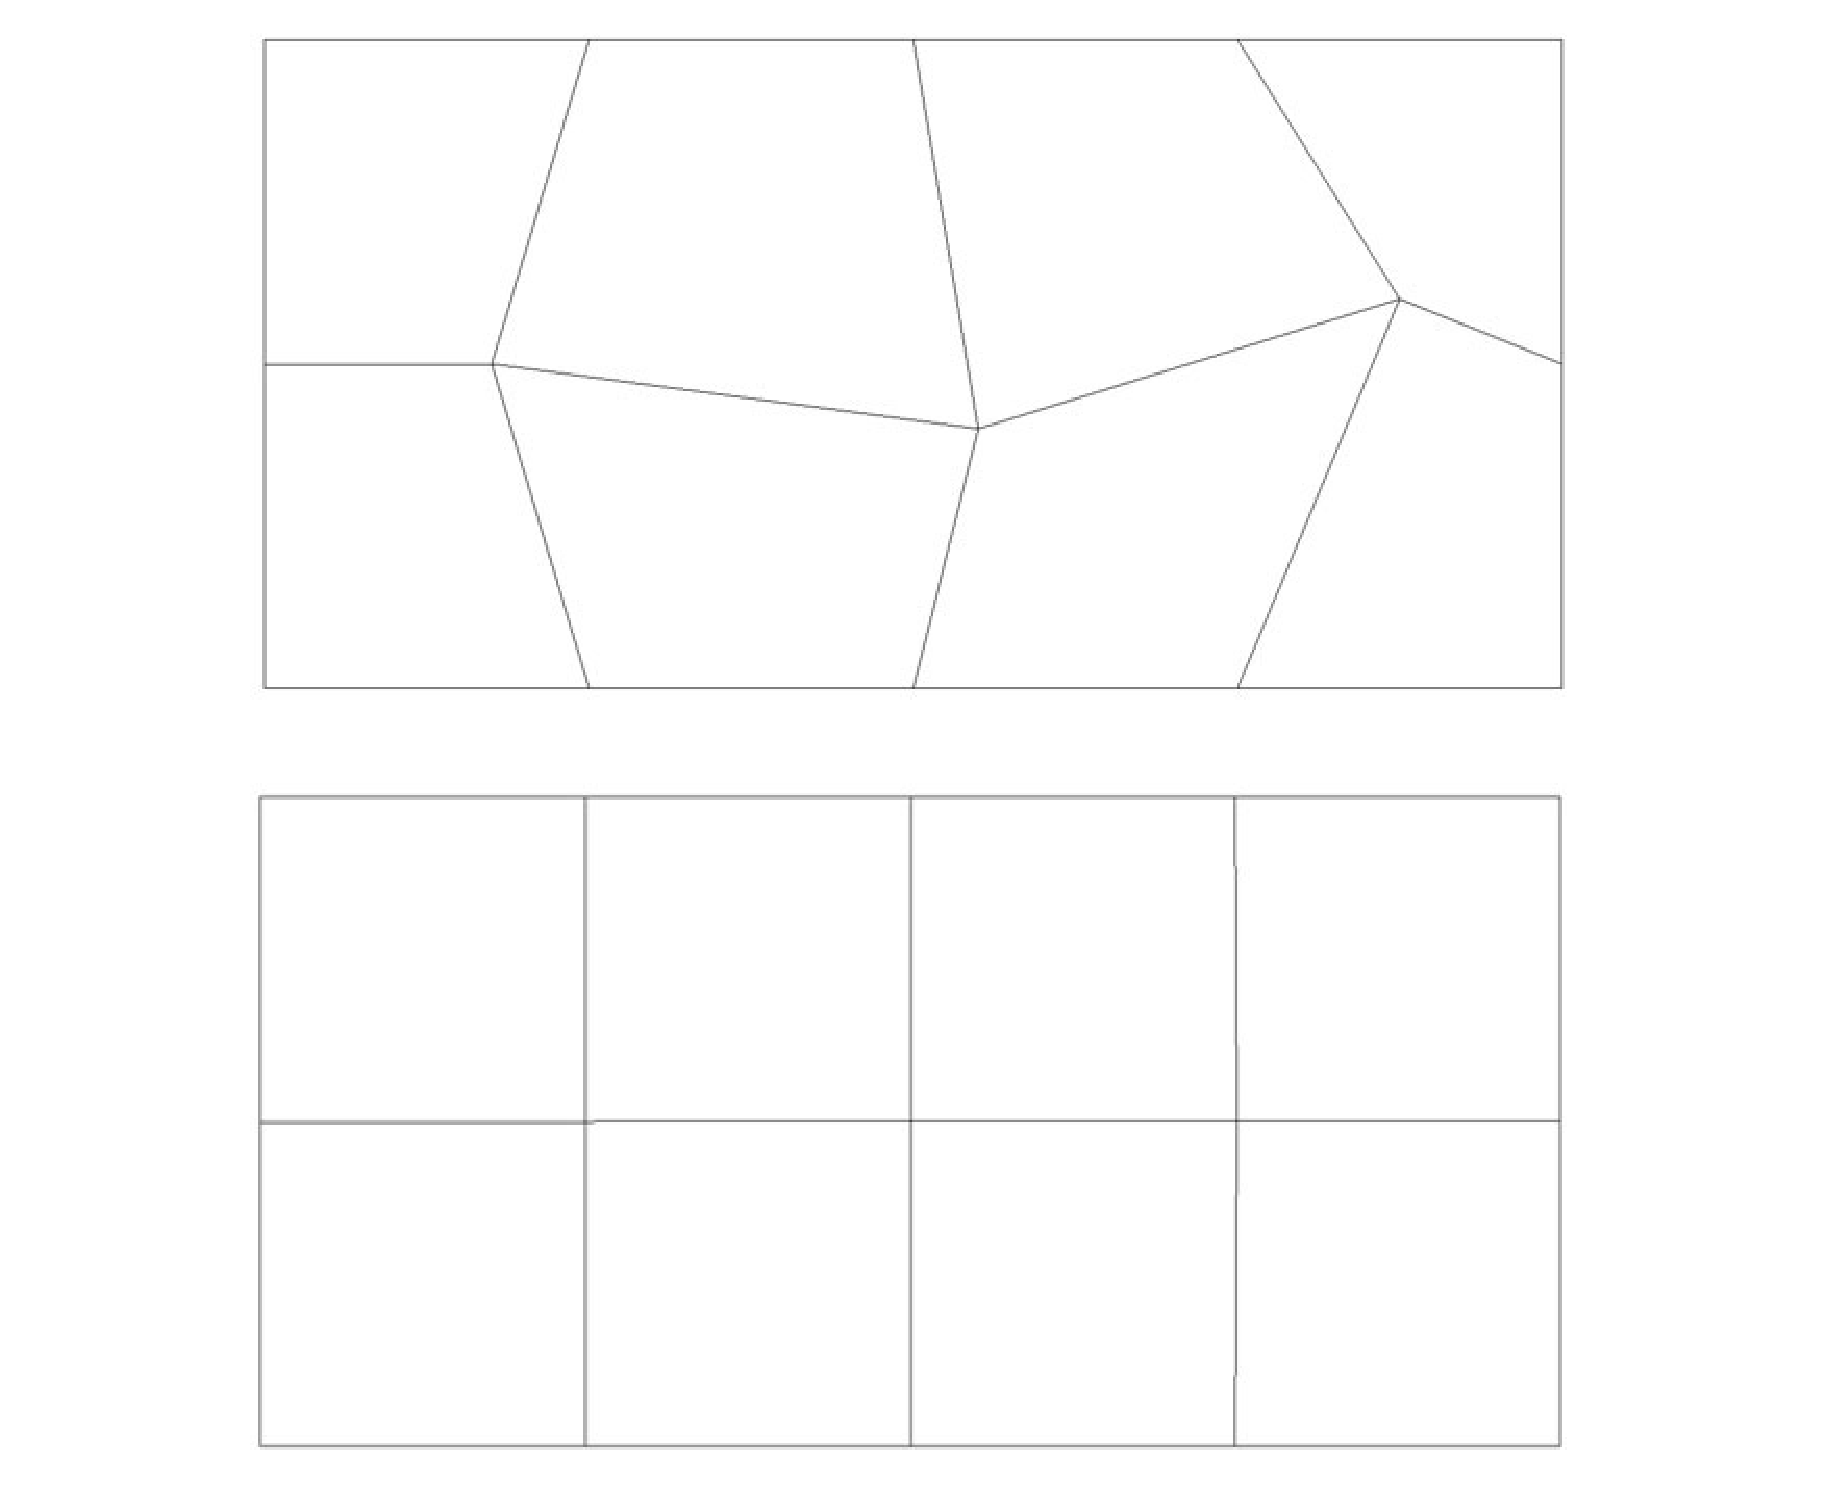
\includegraphics[height=100mm]{figures/min-edge-length}
    \caption{PaverMinEdgeLengthWrapper, file: quads\_4by2\_bad.vtk mesh. The original mesh is on the top, the improved mesh is shown on the bottom.}
    \label{fig:min_edge-length}
\end{center}
\end{figure*}

\newpage

\section{Improve the Shapes in a Size-adapted Mesh} \label{sec:SizeAdaptShapeWrapper}

\noindent {\it Name}: SizeAdaptShapeWrapper \newline
\noindent {\it Purpose}: Make the shape of an element as close as possible to that
of the ideal element shape, {\it while preserving, as much as possible, the size of each element in the mesh}. To be used on isotropic initial meshes that are already size-adapted. \newline
\noindent {\it Notes}: Based on Target-matrix Paradigm. \newline
\noindent {\it Limitations/assumptions}: Initial mesh must be non-inverted.
User wants to preserve sizes of elements in initial mesh and does not want to preserve or
create anisotropic elements.  \newline
\noindent {\it Input Termination Criterion}: maximum iterations (default=50), maximum absolute vertex movement \newline \newline

\noindent Under the Cover: \newline
\noindent {\it Hardwired Parameters}: None \newline
\noindent {\it Metric}: Target2DShapeSizeBarrier or Target3DShapeSizeBarrier \newline
\noindent {\it Tradeoff Coefficient}: 1.0 \newline
\noindent {\it Objective Function}: Linear Average over the Sample Points \newline
\noindent {\it Mesh/Element Type}: Any supported type. \newline
\noindent {\it Solver}: Trust Region \newline
\noindent {\it Global/Local}: Global \newline

\noindent Example: \newline

\begin{verbatim}
************** QualityAssessor(free only) Summary **************

  Evaluating quality for 3456 elements.
  This mesh had 3456 quadrilateral elements.
  There were no inverted elements detected.
  No entities had undefined values for any computed metric.

     Element Quality Statistics

     minimum     average         rms     maximum    std.dev.
  0.00447499     0.23505    0.288066    0.710249    0.166533

     Number of statistics = 3456
     Metric = ElementPMeanP(TShapeSizeB1)
     Element Quality not based on sample points.

    -------------------------------------------
     Element Quality Statistics

     minimum     average         rms     maximum    std.dev.
    0.163072    0.574857     0.62062     1.01908      0.2339

     Number of statistics = 13824
     Metric = EdgeLength
     Element Quality not based on sample points.


************** QualityAssessor(free only) Summary **************

  Evaluating quality for 3456 elements.
  This mesh had 3456 quadrilateral elements.
  There were no inverted elements detected.
  No entities had undefined values for any computed metric.

     Element Quality Statistics

     minimum     average         rms     maximum    std.dev.
  0.00558463   0.0591772   0.0767815    0.303106    0.048923

     Number of statistics = 3456
     Metric = ElementPMeanP(TShapeSizeB1)
     Element Quality not based on sample points.

    -------------------------------------------
     Element Quality Statistics

     minimum     average         rms     maximum    std.dev.
    0.161144    0.562074    0.607611     1.11686    0.230789

     Number of statistics = 13824
     Metric = EdgeLength
     Element Quality not based on sample points.
\end{verbatim}


\begin{figure*}[htbp]
\begin{center}
    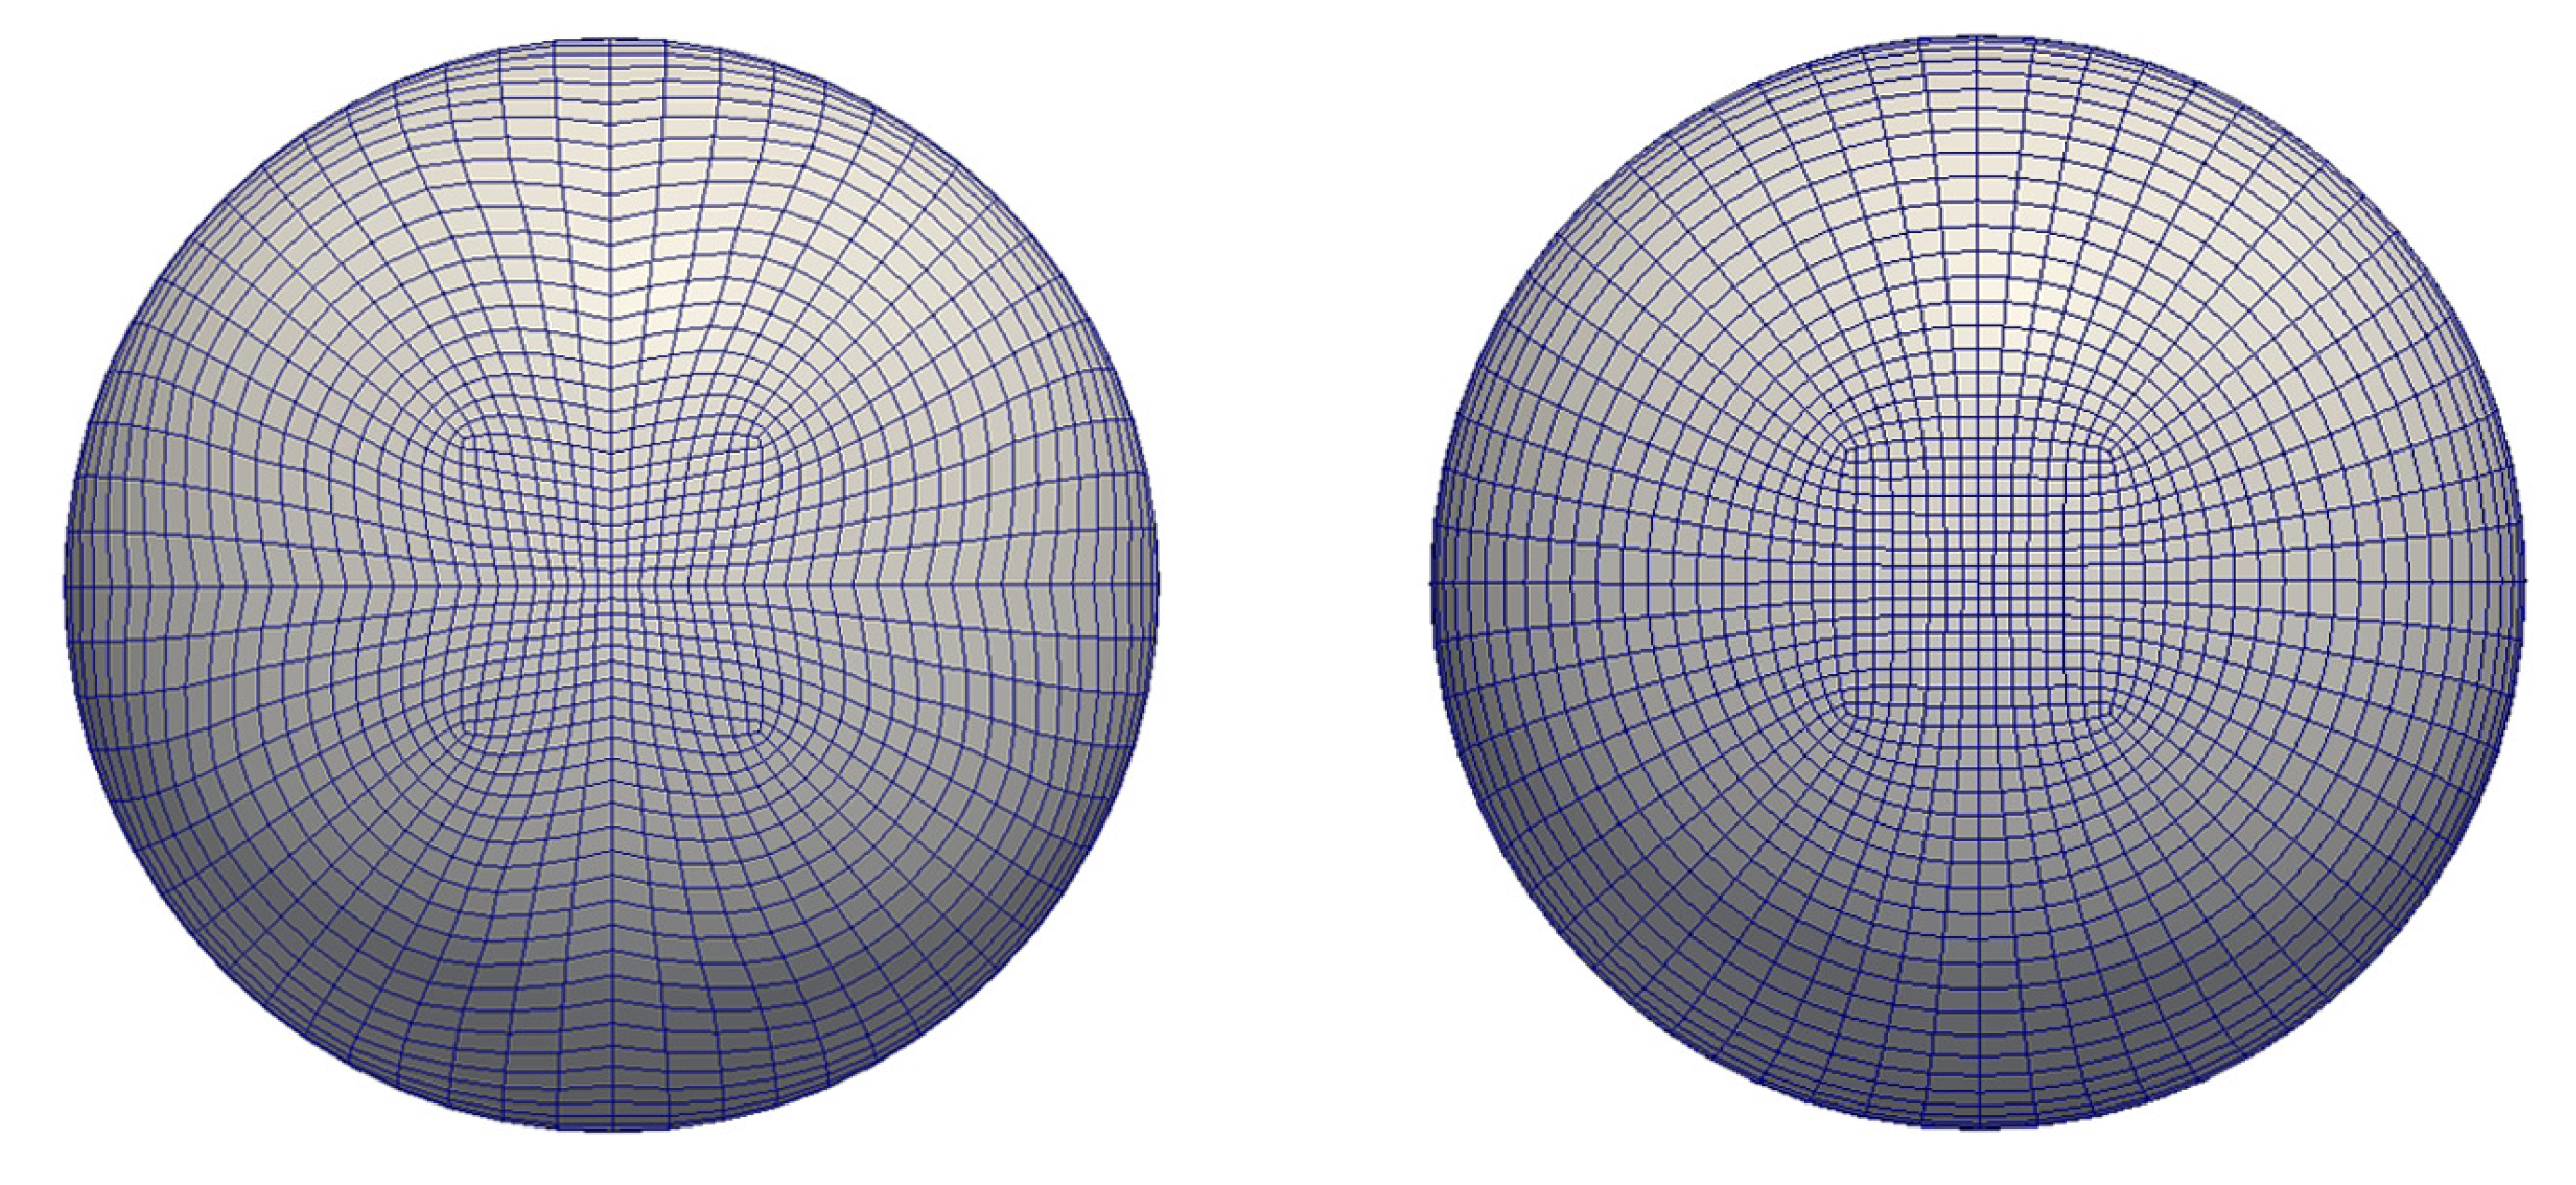
\includegraphics[height=80mm]{figures/bias-sphere-quads}
    \caption{SizeAdaptShapeWrapper, file: bias-sphere-quads.vtk mesh. The original mesh is on the left, the improved mesh is shown on the right.}
    \label{fig:shest_grid32}
\end{center}
\end{figure*}

\newpage

\section{Improve Sliver Tets in a Viscous CFD Mesh} \label{sec:ViscousCFDTetShapeWrapper}

\noindent {\it Name}: ViscousCFDTetShapeWrapper \newline
\noindent {\it Purpose}: Improve the shape of sliver elements in the far-field
of a CFD mesh while
preserving an existing layer of sliver elements in the boundary layer. \newline
\noindent Notes: Based on Target-matrix paradigm.  \newline
\noindent {\it Limitations/assumptions}: Tetrahedral meshes only.  \newline
\noindent {\it Input Termination Criterion}: Iteration Count (default=50) or Maximum Absolution Vertex Movement \newline \newline

\noindent Under the Cover: \newline
\noindent {\it Hardwired Parameters}: In tradeoff coefficient model. \newline
\noindent {\it Metric}: Target2DShape+Target2DShapeSizeOrient (or 3D) (or Barrier) \newline
\noindent {\it Tradeoff Coefficient}: Based on element dihedral angle \newline
\noindent {\it Objective Function}: Linear average over Sample Points \newline
\noindent {\it Mesh/Element Type}: Tetrahedra \newline
\noindent {\it Solver}: Trust Region \newline
\noindent {\it Global/Local}: Global \newline


\noindent Additional Information: \newline
\noindent {\it Article}: Introducing the Target-matrix Paradigm for mesh optimization via node-movement", Engineering with Computers, Sept. 2011.\newline

\newpage
\section{Deforming Domain} \label{sec:DeformingDomain}

\noindent {\it Name}: DeformingDomainWrapper \newline
\noindent {\it Purpose}:  Use initial mesh on undeformed geometric domain
to guide optimization of mesh moved to deformed geometric domain.  \newline
\noindent {\it Notes}: Uses a non-barrier metric which means that the
wrapper could potentially invert/tangle elements.  \newline
\noindent {\it Limitations/assumptions}:  Application responsible for explicit handling of mesh on geometric curves and points.  Initial mesh before moving to deformed domain must be available.\newline
\noindent {\it Input Termination Criterion}: CPU time limit (not used if input
value is non-positive) or fraction of mean edge length (default is 0.005). \newline \newline

\noindent Under the Cover: \newline
\noindent {\it Metric}: TMPQualityMetric(TShapeNB1 or TShapeSizeNB1 or TShapeSizeOrientNB1) \newline
\noindent {\it Objective Function}: Algebraic mean of quality metric values \newline
\noindent {\it Mesh/Element Type}: Any supported type. \newline
\noindent {\it Solver}: Steepest Descent \newline
\noindent {\it Global/Local}: Local with culling \newline

\noindent Additional Information: \newline
\noindent {\it Article}: "Updating meshes on deforming domains",  Communications in Numerical Methods in Engineering, 24:467-476, 2008..\newline

\noindent Example: \newline

\begin{verbatim}
************** QualityAssessor(free only) Summary **************

  Evaluating quality for 216 elements.
  This mesh had 216 quadrilateral elements.
  THERE ARE 56 INVERTED ELEMENTS.
  (Elements invalid at 220 of 864 sample locations.)

  No entities had undefined values for any computed metric.

     Element Quality Statistics

     minimum     average         rms     maximum    std.dev.
4.57621e-005     7.63416     20.8252     67.0217     19.3754

     Number of statistics = 216
     Metric = ElementPMeanP(TShapeNB1)
     Element Quality not based on sample points.


************** QualityAssessor(free only) Summary **************

  Evaluating quality for 216 elements.
  This mesh had 216 quadrilateral elements.
  There were no inverted elements detected.
  No entities had undefined values for any computed metric.

     Element Quality Statistics

     minimum     average         rms     maximum    std.dev.
 0.000763758   0.0202682   0.0252805   0.0947676   0.0151097

     Number of statistics = 216
     Metric = ElementPMeanP(TShapeNB1)
     Element Quality not based on sample points.
\end{verbatim}


\begin{figure*}[htbp]
\begin{center}
    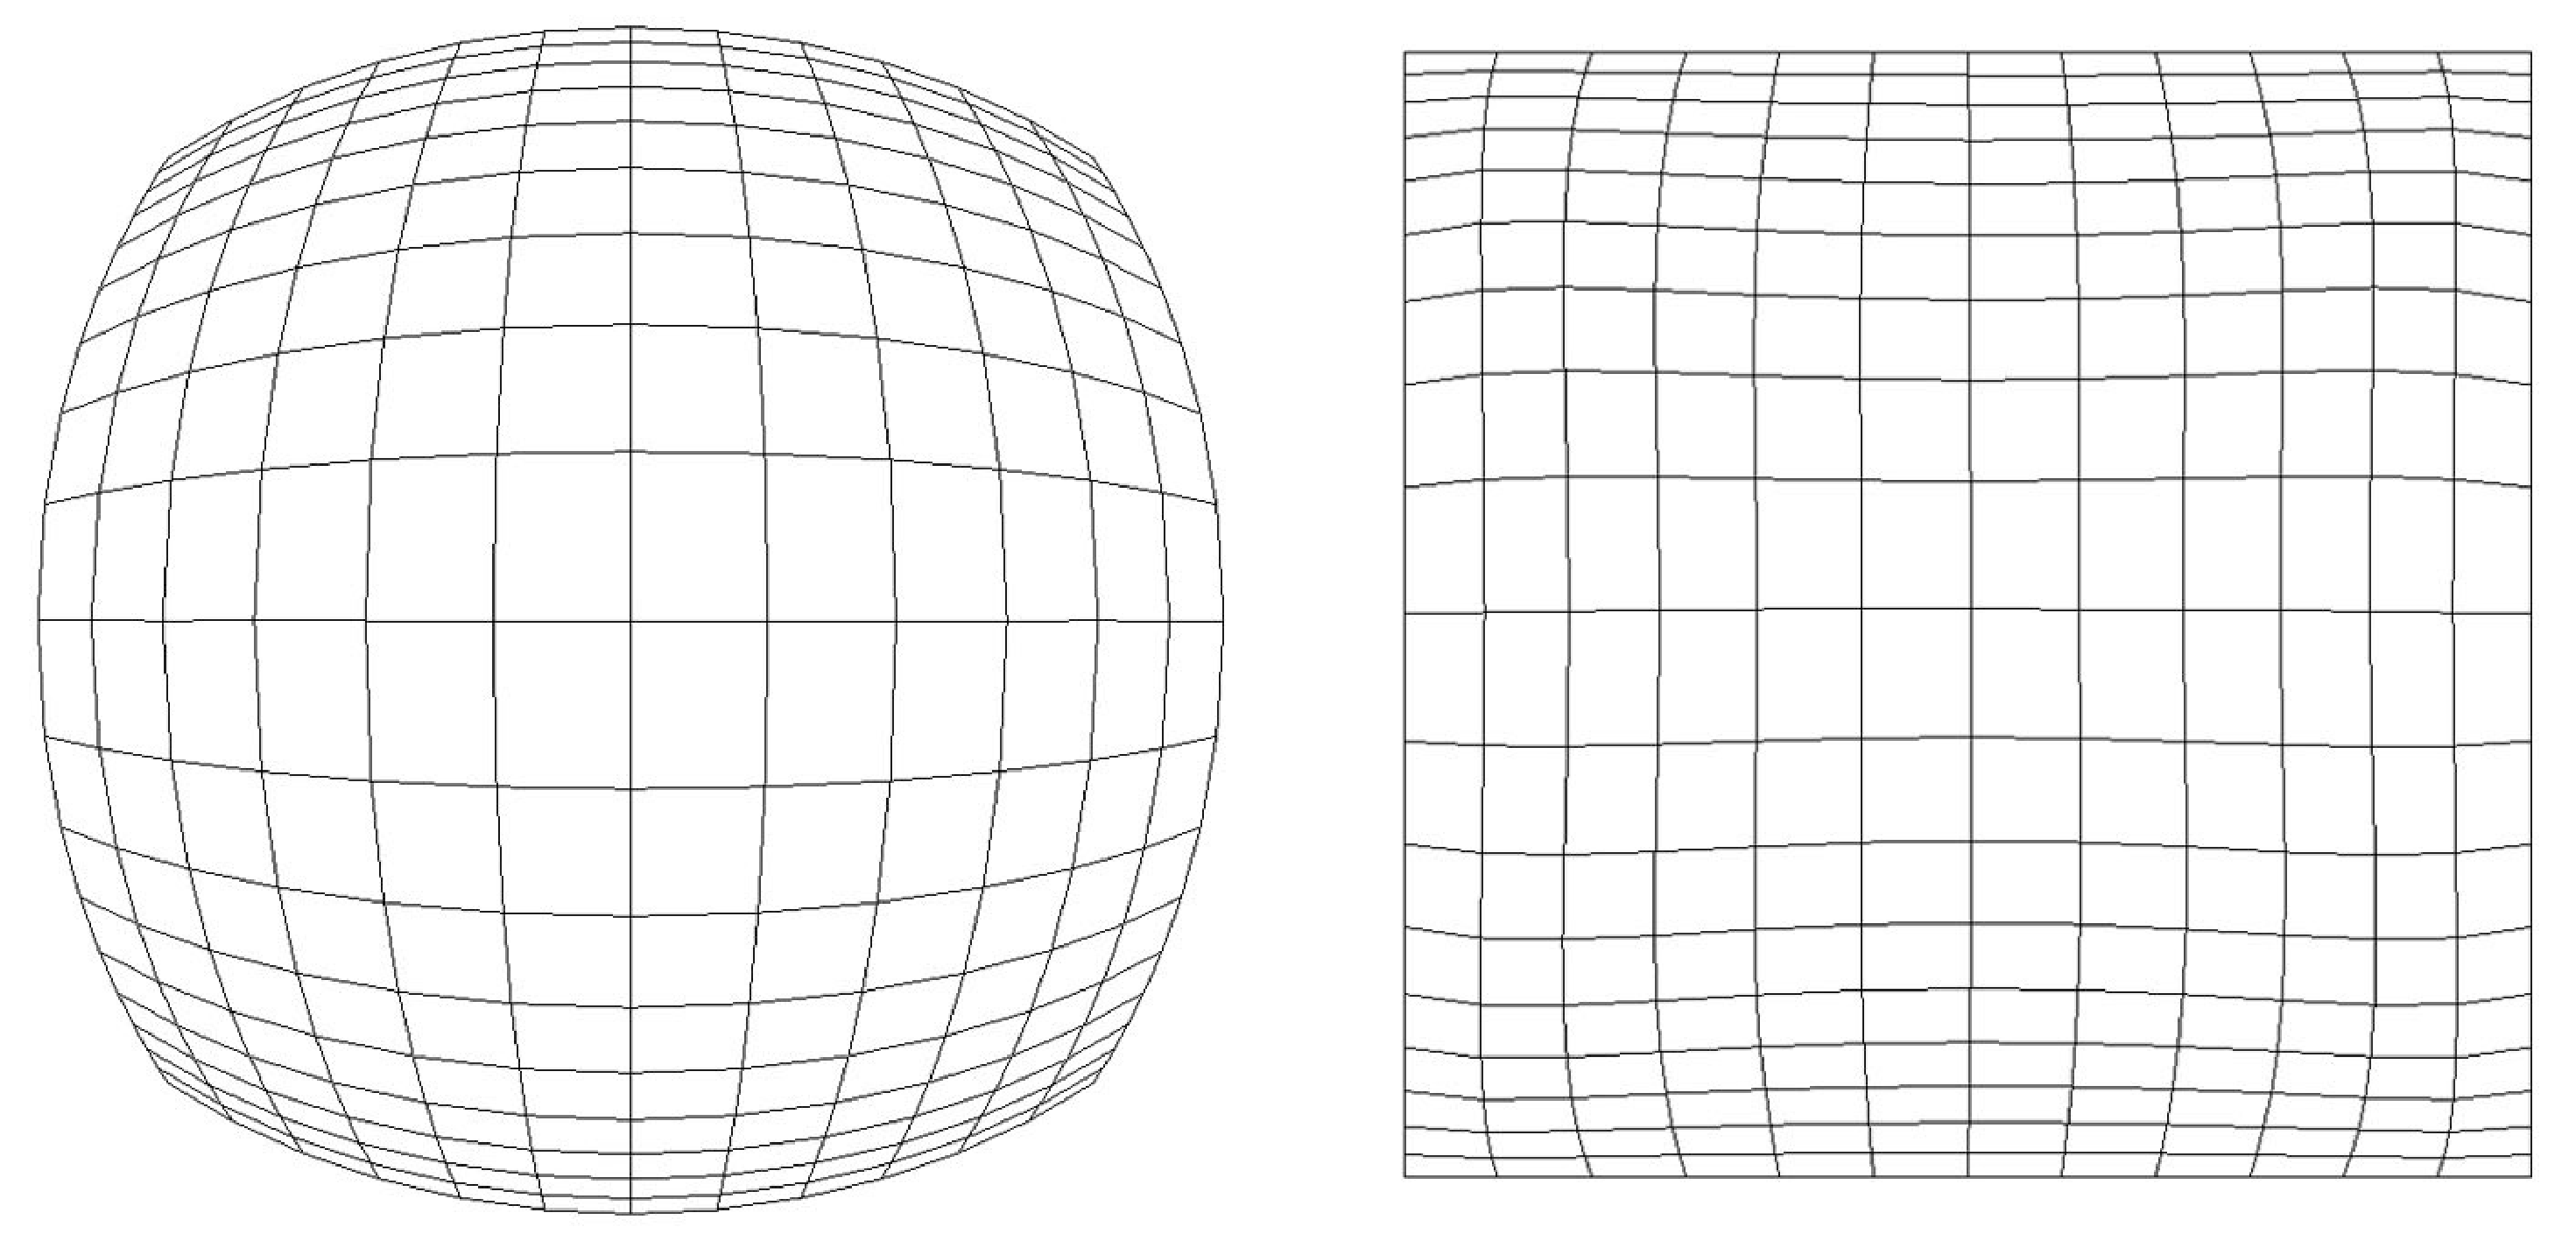
\includegraphics[height=80mm]{figures/sph-10-zsquare}
    \caption{DeformingDomainWrapper, file: sph-10-zsquare.vtk mesh. The original mesh is on the left, the improved mesh is shown on the right.}
    \label{fig:sph-10-zsquare}
\end{center}
\end{figure*}


% Optimization strategies (Nash, global, culling, etc.)
\chapter{Optimization Strategies \label{ch:optstrat}}

\section{The Generalized Optimization Loop}

In Mesquite a generalization of the optimization strategy is used to implement a wide variety of optimization strategies.  Before discussing the different types of optimization strategies that can be implemented with Mesquite we will first need to discuss the generalized strategy.

The mesh can be decomposed into subsets called {\em patches}.  The specifics of this mesh decomposition are discussed in Section \ref{sec:patches}.  The optimization is done by repeatedly iterating over the set of patches, optimizing each separately.

\begin{figure}[htb!]
\begin{center}
\noindent\makebox[\textwidth]{%
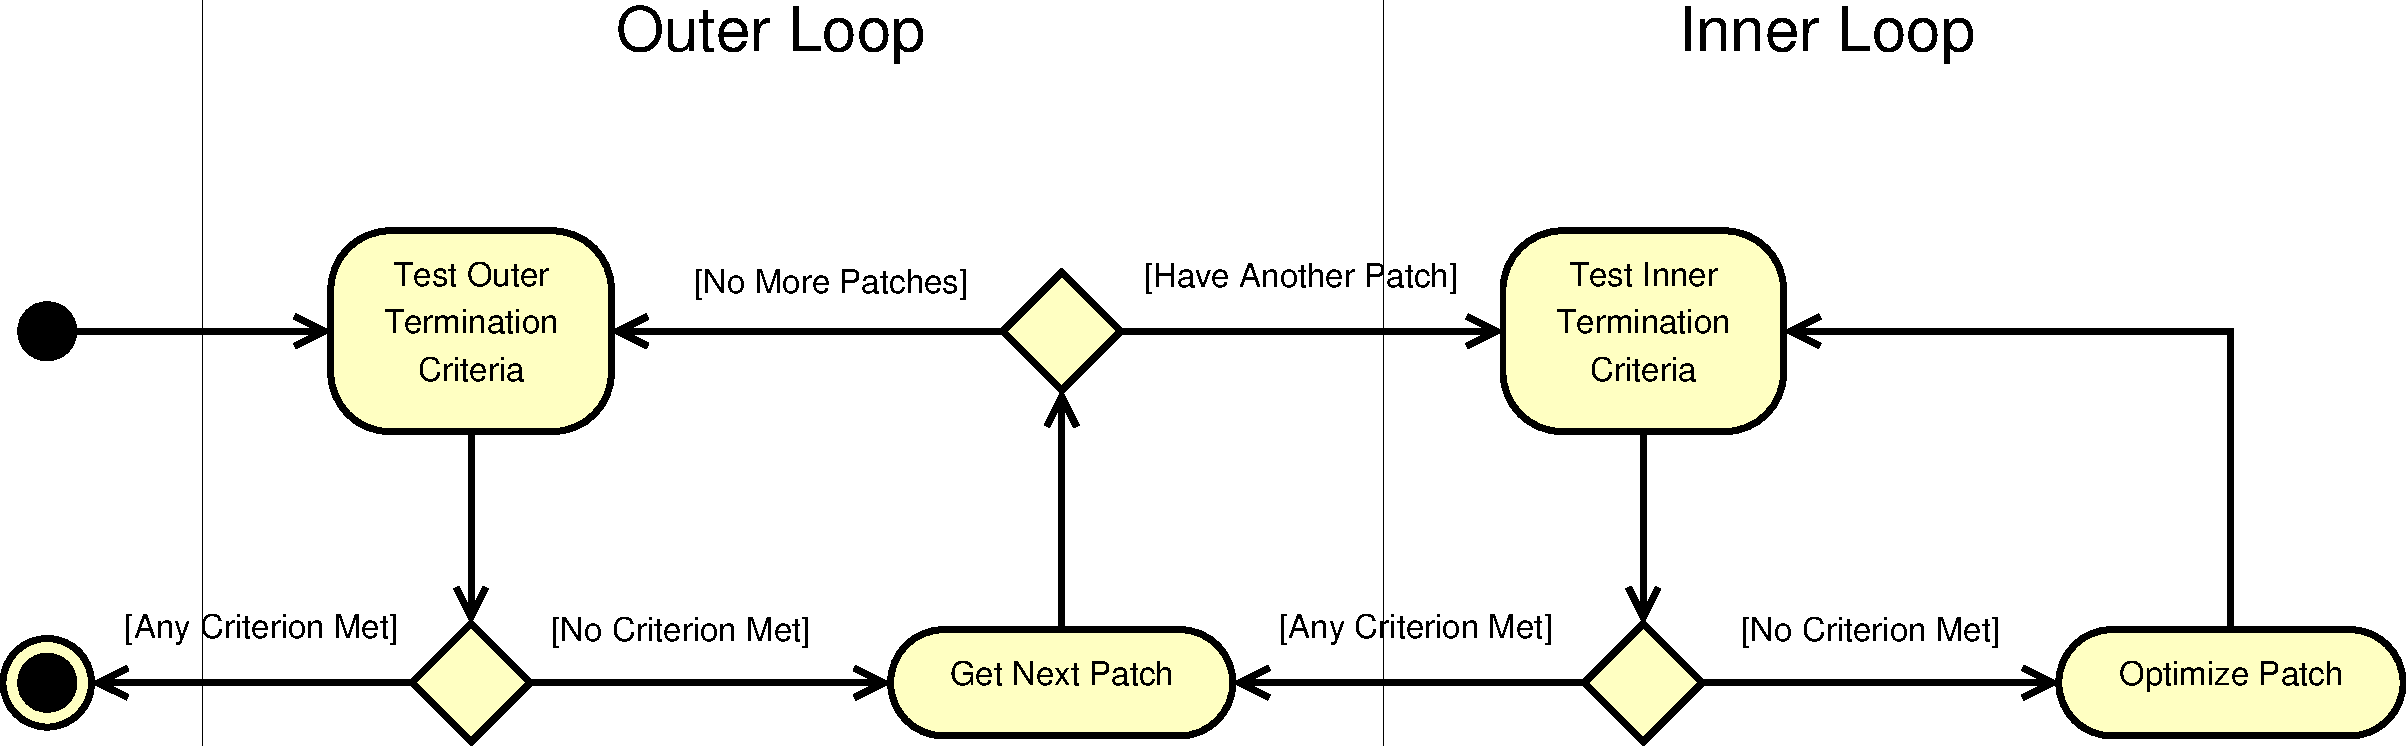
\includegraphics[width=6.5in]{figures/generalized_optimization}}
\caption{\em Optimization Loop \label{fig:genoptloop}}
\end{center}
\end{figure}

Figure \ref{fig:genoptloop} depicts the generalization of optimization strategies in Mesquite.  The generalized optimization is composed of three loops shown as non-overlapping square cycles in the diagram.  The test to exit each loop is performed at the decision points (diamonds) in the diagram.  The loops are logically nested from left to right, such that the right most loop is performed within a single iteration of the loop to the left of it.  The inner- and outer-most loops terminate based on user-definable termination criterion.  The center loop is the iteration over the set of patches composing the mesh.

The inner-most loop (the right-most cycle in the diagram) represents the iterative optimization of the mesh contained in a single patch.  This optimization is done until the {\em inner termination criterion} is met.  Once the inner criterion is met the optimizer advances to the next patch and the inner loop is entered again to optimize that patch.  Once each patch has been optimized the {\em outer termination criterion} is tested.  If the criterion has not been met then the loop over the set of patches is repeated.

The set of outer termination criteria determine when the optimization of the entire mesh is complete.  The set of inner termination criteria determine when the optimization of a single patch is complete.  Both sets of criteria are tested before entering their respective loops.  If a criterion is met before the loop starts then no iterations of the corresponding loop will be performed.

The outer loop(s) are implemented in the {\texttt VertexMover} class.  The inner loop is implemented in subclasses.  The {\texttt LaplacianSmoother} class in Mesquite provides a traditional Laplace smoother.  For this class the mesh is decomposed into patches that each contain a single free vertex and the adjacent elements, one patch for each free vertex in the mesh.  For Laplace smoothing the inner (per-vertex) optimization is not iterative.  The inner loop always has an implicit termination criterion of a single iteration.  Any other inner termination criterion will still be tested before performing the relaxation of the free vertex in the patch such that if any such criterion is met no optimization of the vertex will be performed.  However, culling (Section \ref{sec:culling} can have a similar effect while typically producing better results.  Passes are made over the entire mesh until one of the specified outer termination criterion is met.

\section{Patches \label{sec:patches}}


Mesquite can operate on a decomposition of the mesh into subsets called {\em patches}.  Each patch is optimized individually.  The overall mesh optimization is performed by repeatedly iterating over the set of patches.  Mesquite provides two build-in mesh decompositions\footnote{Mesquite includes an additional decomposition of the mesh into single-element patches which is not suitable for use in optimization.  It is used internally for quality assessment and other purposes}: element-on-vertex patches and a global patch.

\begin{figure}[htb]
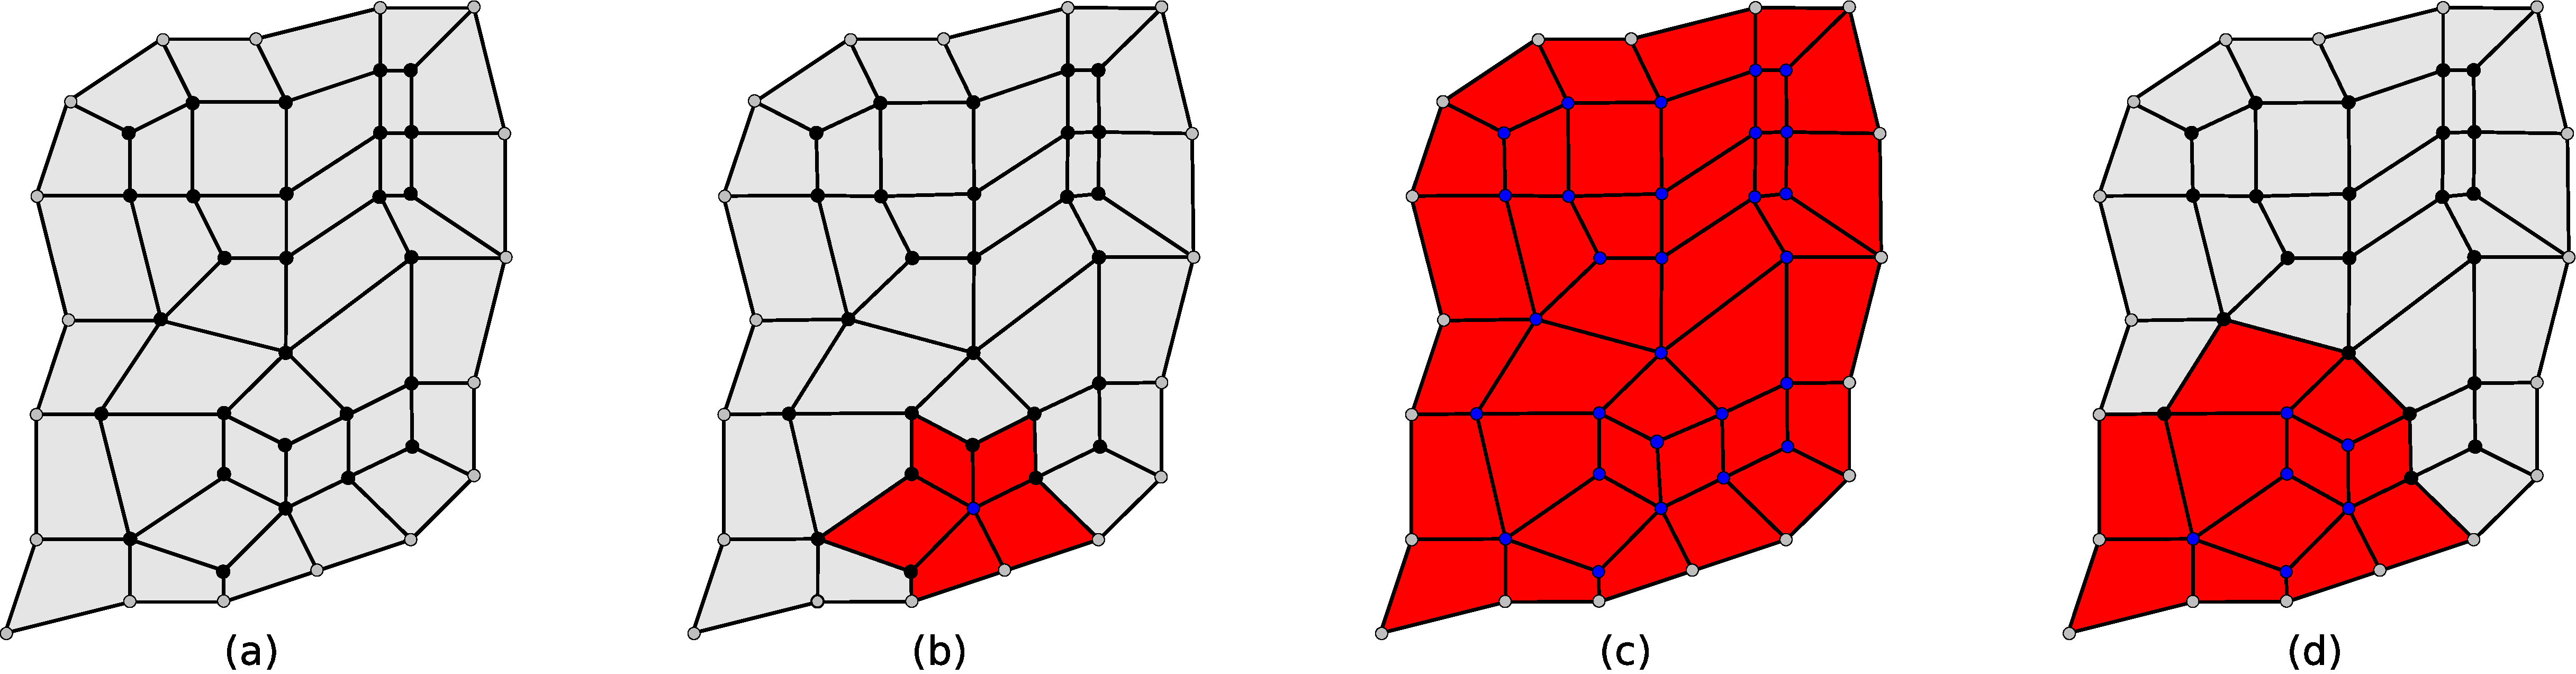
\includegraphics[width=5in]{figures/patches-horiz}
\caption{Miscellaneous patch configurations.\label{fig:patch-types}}
\end{figure}

The global patch is a ``decomposition'' where the entire mesh is contained in a single patch.  This is used in the global optimization strategy discussed in Section \ref{sec:global}. Figure \ref{fig:patch-types}c illustrates the global patch.

The element-on-vertex decomposition subdivides the mesh into a single patch for each free vertex.  Each patch includes the layer of elements adjacent to the free vertex.  A element-on-vertex patch is illustrated in Figure \ref{fig:patch-types}b.  This decomposition is typically used for all optimization strategies discussed in this chapter except for global optimization.  Any other decomposition except global may be used for any of the optimization strategies.  All of the discussed strategies other than global do not make sense for a global patch.

Any patch decomposition can be used with Mesquite.  While no other decomposition strategy is provided with Mesquite, the any implementation of the {\texttt PatchSet} interface can be associated with any quality improver that supports it (any subclass of {\texttt PatchSetUser}, currently all except {\texttt LaplacianSmoother}).  An implementation of that interface is expected to provide three things:
\begin{enumerate}
\item An enumeration of all the patches in the decomposition of the mesh
\item For each patch, the set of vertices to optimize
\item For each patch, the set of elements for which the quality is to be optimized (typically all elements containing the vertices to be optimized.)
\end{enumerate}
A normal decomposition will be done such that each free vertex in the mesh is optimized in exactly one patch, but Mesquite does not enforce this.  Having a free vertex be optimized in no patch will result in that vertex effectively being fixed for the optimization.  A decomposition that optimized the same vertices in multiple patches is allowable, and should have no adverse side effects unless doing a Jacobi optimization (Section \ref{sec:jacobi}).

The listing below shows how a custom implementation of the {\texttt PatchSet} interface can be used with the {\texttt SteepestDescent} solver.

\begin{lstlisting}[frame=single]
MyMeshDecomposition my_patch_set;
SteepestDescent quality_improver( &objective_function );
\<quality_improver.use_patch_set(&my_patch_set);\>
\end{lstlisting}

In any of the examples later in this chapter that call {\texttt use\_element\_on\_vertex\_patch()}, that call may be substituted with a call to {\texttt use\_patch\_set} to use some decomposition other than single-vertex patches.


\section{PatchSetUser and PatchSet}

A \texttt{PatchSetUser} is an optimizer for which the application may specify how the mesh is decomposed into patches.  \texttt{PatchSetUser} provides two pre-defined patch schemes.  The \texttt{use\_global\_patch()} method will result in a single patch containing the entire mesh.  The \texttt{use\_element\_on\_vertex\_patch()} method will result in a patch for every free vertex in the mesh, containing only the free vertex and its adjacent elements.  An alternate scheme for subdividing the mesh into patches may be specified by providing a custom implementation of the \texttt{PatchSet} interface.

The \texttt{PatchSet} interface defines two methods: \texttt{get\_patch\_handles} and \texttt{get\_patch}.  The \texttt{get\_patch\_handles} method returns a list of handles (or identifiers), one for each potential patch in a mesh.  The \texttt{get\_patch} method returns the free vertices and elements in a patch, given one of the handles passed back from the \texttt{get\_patch\_handles} method.

The \texttt{GlobalPatch} class is the implementation of the \texttt{PatchSet} interface that provides a single patch for the entire mesh.  The \texttt{VertexPatches} class provides the Laplacian-like decomposition of the mesh into a patch for every free vertex.  The \texttt{ElementPatches} class is used internally in places other than the main optimization loop, such as initializing BCD data and in the \texttt{QualityAssessor} class.  It decomposes the mesh into single-element patches with no free vertices.


\section{Global \label{sec:global}}

For a global optimization an objective function that measures the quality of the mesh is minimized using a numerical solver.  The coordinates of all of the free vertices in the mesh are the free variables in the optimization.  This is the default mode of operation for most solver-based implementations of the {\texttt QualityImprover} interface.

A global optimization is simplest form of the generalized optimization loop.  In this mode the mesh is ``decomposed'' into a single patch containing the entire mesh.  The outer loops in Figure \ref{fig:genoptloop} are executed only once.  The entire optimization process happens in the inner loop.  For global optimization the outer termination criterion is the default of a single iteration.  The inner termination criterion should be used to terminate the optimization process.  Setting some other outer termination criterion is not prohibited, but will result in a much less efficient optimization process.  There is no logical difference between inner and outer termination criterion, but each iteration of the outer loop begins with a clean solver state which will result in less efficient operation of the solver.  Even steepest descent, the simplest solver, calculates a initial step size based on the previous iteration of the inner loop.

The listing below shows how global optimization can be selected.

\begin{lstlisting}[frame=single]
// Create global optimizer instance
SteepestDescent improver( &objective_function );
\<improver.use_global_patch();\>

// Set only inner termination criterion for
// global optimization
TerminationCriterion inner;
inner.add_absolute_vertex_movement( 1e-3 );
improver.set_inner_termination_criterion( &inner );

// Run optimization
InstructionQueue queue;
queue.set_master_quality_improver( &improver, err );
queue.run_instructions( &mesh, err );
\end{lstlisting}


\section{Nash Game vs. Block Coordinate Descent}

Quality improvers that have an explicit \texttt{ObjectiveFunction} may be used with the block coordinate descent algorithm rather than the default Nash game algorithm if the \texttt{ObjectiveFunction} implementation supports this mode of operation. In a Nash game optimization (the default), the objective function that is optimized by the inner loop is evaluated over only the patch being optimized.  In a block coordinate descent algorithm, the objective function to be optimized in the inner loop is evaluated over the entire mesh.  Only the influence of the current patch vertices on the global objective function is considered during the optimization of each patch.

\section{Nash Game \label{sec:nash} }


\begin{lstlisting}[frame=single]
// Create Nash optimizer instance
SteepestDescent improver( &objective_function );
\<improver.use_element_on_vertex_patch();\>

// Set inner and outer termination criterion for
// non-global patch
TerminationCriterion inner, outer;
outer.add_absolute_vertex_movement( 1e-3 );
inner.add_iteration_limit( 2 );
improver.set_outer_termination_criterion( &outer );
improver.set_inner_termination_criterion( &inner );

// Run optimization
InstructionQueue queue;
queue.set_master_quality_improver( &improver, err );
queue.run_instructions( &mesh, err );
\end{lstlisting}


\section{Block Coordinate Descent \label{sec:bcd} }

\begin{lstlisting}[frame=single]
// Create BCD optimizer instance
SteepestDescent improver( &objective_function );
improver.use_element_on_vertex_patch();
\<improver.do_block_coordinate_descent_optimization();\>

// Set inner and outer termnation criterion for
// non-global patch
TerminationCriterion inner, outer;
outer.add_relative_quality_improvement( 1e-2 );
inner.add_iteration_limit( 2 );
improver.set_outer_termination_criterion( &outer );
improver.set_inner_termination_criterion( &inner );

// Run optimization
InstructionQueue queue;
queue.set_master_quality_improver( &improver, err );
queue.run_instructions( &mesh, err );
\end{lstlisting}


\section{Culling \label{sec:culling}}


\begin{lstlisting}[frame=single]
// Create Nash optimizer with culling
SteepestDescent improver( &objective_function );
improver.use_element_on_vertex_patch();

// The culling criterion is effectively an outer
// termination criterion because optimization will
// always stop when all patches are culled.  We
// must explicitly pass an empty outer termination
// criterion to replace the default of one iteration.
// Additional outer termination criteria may also be
// specifed.
TerminationCriterion inner, outer;
\<inner.cull_on_absolute_vertex_movement( 1e-3 );\>
inner.add_iteration_limit( 2 );
improver.set_outer_termination_criterion( &outer );
improver.set_inner_termination_criterion( &inner );

// Run optimization
InstructionQueue queue;
queue.set_master_quality_improver( &improver, err );
queue.run_instructions( &mesh, err );
\end{lstlisting}

\section{Jacobi \label{sec:jacobi}}

\begin{lstlisting}[frame=single]
// Create Jacobi optimizer instance
SteepestDescent improver( &objective_function );
improver.use_element_on_vertex_patch();
\<improver.do_jacobi_optimization();\>

// Set inner and outer termination criterion for
// non-global patch
TerminationCriterion inner, outer;
outer.add_absolute_vertex_movement( 1e-3 );
inner.add_iteration_limit( 2 );
improver.set_outer_termination_criterion( &outer );
improver.set_inner_termination_criterion( &inner );

// Run optimization
InstructionQueue queue;
queue.set_master_quality_improver( &improver, err );
queue.run_instructions( &mesh, err );
\end{lstlisting}



% Constructing custom solvers - part 1
%\input{custom.tex}

% TMP
%\input{tmp.tex}

% more TMP stuff
%\input{more_tmp.tex}

% debugging solvers
\chapter{Analyzing Optimizer Behavior}

This chapter provides a brief overview of some of the tools provided in Mesquite for assisting with the analysis and visualization of the Mesquite optimization process.  The tools discussed in this section can be used to provide additional output.	 External tools such as Paraview, VisIt, or GNU Plot must be used to visualize the data.

\section{Assessing Quality}

  The QualityAssessor class provides a summary of the mesh quality. It can be used with Non Target-paradigm metrics (QualityMetric classes) as well as Target-paradigm metrics (TMetric classes). For simplicity, the following discussion refers to the QualityMetrics classes but the concepts apply to the TMetric classes as well.	The QualityAssessor class can be used in a direct fashion as shown in the example below or via the InstructionQueue class as described in Section \ref{sec:tutDetailedAPI}.  An instance of the QualityMetric class can be specified for the QualityAssessor instance at creation to be used to assess the mesh quality.  Additional QualityMetric instances can be created using the Assessor class and by adding them to the QualityAssessor instance via the "add\_quality\_assessment" method. If no QualityMetrics are specified, the only assessment that will be performed is a simple count of inverted elements. One or more instances of the QualityAssessor class may be inserted in the InstructionQueue at any point to print a summary of the mesh quality at that time during the optimization.

\subsection{Stopping Assessment}

A stopping assessment can be specified for each QualityAssessor instance.  The "stopping assessment" directs the assessment code calculate a value using the power mean data to use that value as the return value for the loop\_over\_mesh call.  If no power mean is specified for a QualityAssessor instance, a simple average of all metric values calculated during the assessment is returned from  loop\_over\_mesh.  Only one stopping assessment with its associated power mean can be specified for a particular QualityAssessor instance.  There are three different ways to specify a stopping assessment: when the QualityAssessor instance is created using a constructor, when a quality assessment is added via the add\_quality\_assessment () method, and directly with the set\_stopping\_assessment() method.  Since only one stopping assessment can be defined for a each instance of QualityAssessor, the last action that causes the stopping assessment to be set will be the one used for the assessment no matter how many metrics have been included.

\subsection{Using the Quality Assessor}
\label{sec:using_qa}

  The QualityAssessor class provides a number of constructors.	Each allows the specification of a different set parameters to control the quality assessment.	The parameters are described below including default values, if any. Note that all parameters are not used in each constructor.

\label{QA_params}
Parameters used by QualityAssesor constructors:
\begin{description}
\item[metric:]	 QualityMetric to register for use in assessing mesh quality.  Will also be used in the setting of the stopping assessment.

\item[histogram\_intervals:]   If non-zero, a histogram of quality metric values composed of the specified number of intervals will be generated.  Default is zero.
\item[power\_mean:] If non-zero, in addition to the normal summary statistics for the quality metric, an additional general power mean with the specified power will be calculated.  Is used as the value set for the stopping assessment.  Default is zero.

\item[free\_elements\_only:] When this option is TRUE, summary statistics are only computed over the set of elements which contain free vertices. If an element in the mesh does not contain a free vertex, its quality is not included in the summary.	 If an element in the mesh does not contain a free vertex, its quality cannot be improved by Mesquite.	To compute the quality of all mesh elements, regardless of whether Mesquite can improve them, set this option to FALSE.	 Default is TRUE.

\item[metric\_value\_tag\_name:] If a non-null value is specified, a tag with the specified name can be associated with quality values for individual elements or vertices if metric is an element-based or vertex-based metric.  If metric is not element-based or vertex-based, this argument has no effect. The specified tag can then be associated with quality values generated for a mesh.  Element-based metrics can have one tagged value per element quality value while vertex-based metrics can have one tagged value per vertex quality value.  Tagged quality values are created using the methods tag\_set\_element\_data() and tag\_set\_vertex\_data() found in the MeshImpl class. The tagged values can be retrieved using the methods tag\_get\_element\_data() and tag\_get\_vertex()\_data from the same class.  Tags cannot be used with target metric classes. Default for metric\_value\_tag\_name is null value.

\item[inverted\_element\_tag\_name:] If a non-null value is specified, an integer tag with the specified name will be used to store a value of 0 for normal elements and 1 for inverted elements.  Default is null value.

\item[print\_summary\_to\_std\_out:] If TRUE, summary of mesh quality will be written to std::out.  If FALSE, quality assessment will be available via the get\_results and get\_all\_results methods, but will not be printed.	 Default is TRUE.

\item[output\_stream IO:] stream to which to write a summary of the mesh quality.

\item[name:] Name to include in output.	 Useful if several QualityAssessors are in use at the same time.
\end{description}

  After the QualityAssessor instance is created, any of a number of methods can be used to set individual characteristics of the QualityAssessor object.

The add\_histogram\_assessment method can be used to assign values for a histogram.  If the specified QualityMetric instance has not been added to the QualityAssessor instance, it will be created with the provided values.  If the QualityMetric instance was previously added to the QualityAssessor instance, it is updated with the provided values. The signiture of the method is:

\begin{verbatim}

  void add_histogram_assessment( QualityMetric* qm,
                                 double min,
                                 double max,
                                 int intervals,
                                 double power_mean = 0.0,
                                 const char* metric_value_tag_name = 0,
                                 const char* metric_label = 0 );

\end{verbatim}

The paramaters min and max are used to define the lower and upper limits for the values displayed in the histogram.  If zero, the value used for the histogram will be based on the actual values of the quality assessment.  The intervals parameter specifies how many "steps" or "bins" will be shown on the histogram.  If the specified value is negative or 0, an interval of one will be used. The metric\_label parameter is a string that will be used to identify the historgram in the output. It is useful when several quality assessments are used at the same time.  The remaining parameters work as described in Section \ref{sec:using_qa}.


  Once setup for the QualityAssessor object is complete, the actual assessment is preformed by calling "loop\_over\_mesh".  After it terminates, results can be obtained using various methods supplied by the QualityAssessor class.

For each instance of the QualityAssessor, a summary of the results will be printed after the assessments have been completed. Display of the summary can be turned off by calling disable\_printing\_results() before the assessment is started.  The summary will include data for each of the metric assessments run by the Assessor.	 The printed data includes the metric name, the minimum and maximum values, the average value, the rms (root mean square), and the standard deviation.	If a power mean was specified for the assessment, an additional column will display the resultant value under a header containing the power mean value used in the calculation.	  All values in the QualityAssessor summary table are per mesh element.	 Any requested histograms are then displayed.  The number of values in the histogram is dependant upon the type of metric performed.  For element-based metrics, the histogram contains one value per element.	For vertex-based metrics, it will contain the number of target sample points per element times the number of elements.

Element quality metrics is calculated in one of  four ways:


\begin{enumerate}
\item As the average of the quality values of the underlying sample points.  A single quality value is calculated for each element.  This functionality is provided by the ElementAvgQM class.
\item As the maximum of the quality values of the underlying sample points for each element.  A single quality value is calculated for each element.  This functionality is provide by the ElementMaxQM class.
\item For target-based metrics (any metric derived from the TMPQualityMetric class or TMetric class used in conjuntion with the TQualityMetric class),  a quality value is produced for each element sample point.  For example, a quadrangle has four sample points, one at each corner, therefore four quality values per element will be produced for a quadrangle when using a target-based metric.
\item All other metrics derived from the QualityMetric class that are not one of the above metrics will have one quality metric value per element.  Sample points are not used.
\end{enumerate}


  Below is an example of a summary and histogram for an eight element mesh for two different metrics, one that included a power mean of 1.5.


\begin{verbatim}

************** QualityAssessor(free only) Summary **************

  Evaluating quality for 8 elements.
  This mesh had 8 quadrilateral elements.
  There were no inverted elements detected.
  No entities had undefined values for any computed metric.

     Element Quality Statistics

     minimum     average         rms     maximum    std.dev.
     1.05817     1.14257      1.1469     1.35948   0.0995044

     Number of statistics = 8
     Metric = Condition Number
     Element Quality not based on sample points.

    -------------------------------------------
     Sample Point Quality Statistics

     minimum     average     1.5-mean         rms     maximum    std.dev.
        1.18        2.23      2.28262     2.33533        3.77    0.693433

     Number of statistics = 32
     Metric = TSquared


   TSquared histogram:
   (  1-1.3) |======================3
   (1.3-1.6) |==============================4
   (1.6-1.9) |==============================4
   (1.9-2.2) |====================================================================9
   (2.2-2.5) |===============2
   (2.5-2.8) |==============================4
   (2.8-3.1) |=======1
   (3.1-3.4) |======================3
   (3.4-3.7) |=======1
   (3.7-4  ) |=======1
  metric was evaluated 32 times.

\end{verbatim}

\section{QualityMetrics Classes}

The QualityMetric classes are divided into groups based on their general function as detailed in the following sections.

\subsection{Shape Quality Metrics}

\subsubsection{AspectRatioGammaQualityMetric}

This class computes the Aspect Ratio Gamma metric for two- and three-diminsional simplicial elements.

\subsubsection{ConditionNumberQualityMetric}

  Computes the condition number of given element.

     The metric does not use the sample point functionality or the compute\_weighted\_jacobian.  It evaluates the metric at  the element vertices, and uses the isotropic ideal element. It does require a feasible region, and the metric needs to be minimized

\subsubsection{IdealWeightInverseMeanRatio}

Computes the inverse mean ratio of given element.

The metric does not use the sample point functionality or the compute\_weighted\_jacobian.  It evaluates the metric at the element vertices, and uses the isotropic ideal element.  Optionally, the metric computation can be raised to the 'pow\_dbl' power.  This does not necessarily raise the metric value to the 'pow\_dbl' power but instead raises each local metric.  For example, if the corner inverse mean ratios of a quadraliteral element were m1,m2,m3, and m4 and we set pow\_dbl=2 and used linear averaging, the metric value would then be m = .25(m1*m1 + m2*m2 + m3*m3 + m4*m4).  The metric does require a feasible region, and the metric needs to be minimized if pow\_dbl is greater than zero and maximized if pow\_dbl is less than zero.  pow\_dbl being equal to zero is invalid.

\subsubsection{IdealWeightMeanRatio}

Computes the mean ratio quality metric of given element.

 The metric does not use the sample point functionality or the     compute\_weighted\_jacobian.  It evaluates the metric at the element vertices, and uses the isotropic ideal element.  It does require a feasible region, and the metric needs to be maximized.

\subsection{TMP Quality Metrics}

\subsubsection{AffineMapMetric}

Compares targets to affine map to ideal element.

A quality metric defined using 2D and 3D target metrics, where the active (A) matrix is an affine map to the ideal, unit-side element.

\subsubsection{AWQualityMetric}

Compares targets to mapping function Jacobian matrices

 A quality metric defined using 2D and 3D target metrics, where the active (A) matrix compared to the target by the underlying metrics is the Jacobian matrix of the mapping function at a given sample point.  For surface elements, A is rotated to align the normal with W, such that both matrices can be reduced from 3x2 to 2x2.

\subsubsection{TMPQualityMetric}

Compare targets to mapping function Jacobian matrices

 Base class for various TMP QualityMetric implementations.

\subsubsection{TQualityMetric}

Compare targets to mapping function Jacobian matrices

A quality metric defined using 2D and 3D target metrics, where the active (A) matrix compared to the target by the underlying metrics is the Jacobian matrix of the mapping function at a given sample point.  For surface elements, A is rotated to align the normal with W, such that both matrices can be reduced from 3x2 to 2x2.

\subsection{Untangle Quality Metrics}

\subsubsection{UntangleBetaQualityMetric}

  The untangle beta quality metric.

  Given a scalar value beta and local signed element volume alpha\_i, define delta\_i to be alpha\_i minus beta.  The Untangle beta value is then defined as square root of the sum over sample points of the absolute value of delta\_i minus delta\_i, difference squared. That is, the root mean square of the difference, abs(delta\_i) minus delta\_i.

The constructor defaults to RMS AveragingMethod and ELEMENT\_VERTICES evaluationMode.  The default beta value is .05.

\subsection{Volume Quality Metrics}

\subsubsection{LocalSizeQualityMetric}

  Computes the local size metric for a given vertex.

  LocalSizeQualityMetric is a vertex based metric which computes the corner volume (or area) for the element corners attached to a given element.  Then these volumes (or areas) are averaged together.  The default averaging method is QualityMetric::RMS.

\subsubsection{SizeMetric}

Element size (area or volume)

This metric is intended primarily for use with QualityAssessor for obtaining a summary of the element sizes in the mesh.



\clearpage
\section{Quality Assessor Code Example}

A simple example using the QualityAssessor class:

\begin{lstlisting}[frame=single]
  MsqError err;
  MeshImpl meshToAssess;
  PlanarDomain myDomain;
  Settings mySettings;

  meshToAssess.clear();

    // read in mesh
  const char* filename = "meshToAssess.vtk";
  meshToAssess.read_vtk( filename, err);

    // create metric instance
  ConditionNumberQualityMetric metric;

    // create QualityAssessor instance accepting default values
  QualityAssessor qa( &metric );

    // change some of the default parameters
  qa.measure_free_samples_only( false );
  qa.disable_printing_results();

    // run the QualityAssessor
  MeshDomainAssoc mesh_and_domain = MeshDomainAssoc(&meshToAssess, &myDomain);
  qa.loop_over_mesh( &mesh_and_domain, &mySettings, err );

    // get results
  const QualityAssessor::Assessor* results = qa.get_results( &metric );
  int invalid_element_count = results->get_invalid_element_count();
  if ( invalid_element_count != 0 )
    std::cout << "Warning: " << invalid_element_count
			<< " invalid elements found." << std::endl;
\end{lstlisting}

\section{Common-scale Histograms}

When optimizating a mesh, it can be useful to display the quality before and after optimization.  This is done by adding a QualityAssessor instance to an InstructionQueue, adding a quality improver instance to the InstructionQueue, and then adding the Quality Assessor instance to the InstructionQueue a second time.  This allows a comparison of the mesh quality before and after optimization.  Example code for doing this:

\begin{lstlisting}[frame=single]
#include "Mesquite_all_headers.hpp"

using namespace Mesquite;

int main()
{
  MsqPrintError err(std::cout);
  Mesquite::MeshImpl mesh;
  mesh.read_vtk("hexes_4by2by2.vtk", err);

  ConditionNumberQualityMetric cond_num;

    // builds an objective function
  LPtoPTemplate obj_func(&cond_num, 2, err);
  if (err) return 1;

    // creates the steepest descent optimization procedures
  SteepestDescent descent_method( &obj_func );
  descent_method.use_global_patch();

  QualityAssessor qa=QualityAssessor(&cond_num, 10);
  if (err) return 1;

    //**************Set termination criterion****************
  TerminationCriterion tc2;
  tc2.add_iteration_limit( 1 );
  descent_method.set_inner_termination_criterion(&tc2);

    // creates an instruction queue
  InstructionQueue queue1;

    // adds quality assessment to instruction queue
  queue1.add_quality_assessor(&qa,err);

    // adds a improver/solver to instruction queue
  queue1.set_master_quality_improver(&descent_method, err);
  if (err) return 1;

    // adds another quality assessment to instruction queue
    // to show any improvement
  queue1.add_quality_assessor(&qa,err);
  if (err) return 1;

    // launches optimization on mesh
  queue1.run_instructions(&mesh, err);
  if (err) return 1;

  return 0;
}
\end{lstlisting}


\subsection{Creating Common-scale Histograms}
\label{sec:creating_histograms}

Comparing before and after histograms can be difficult when there is a large difference in the resultant quality value range.  In such cases, the common-scale histogram feature can be used to display two histograms with a common vertical interval scale and a common horizontal scale for the number of quality values that fall into each interval.  Unlike the above example that reused the same QualityAssessor instance for the before and after histograms, the common-scale histograms require two separate QualityAssessor instances.  After both the before optimization and after optimization quality assessments have been performed, the method 'scale\_histograms(QualityAssessor* optimal)' can be called to create a pair of common-scale histograms.  The before assessment is known as the 'initial', the after assessment is known as the 'optimal'.   The histogram interval for both the initial and optimal assessments must be the same for scale\_histograms() to work correctly.

 Below is a portion of the previous code modified to show how to create common-scale histograms.
\begin{lstlisting}[frame=single]
    // Set up the quality assessors
  QualityAssessor initial_quality_assessor=QualityAssessor(&cond_num, 10);
  QualityAssessor optimal_quality_assessor=QualityAssessor(&cond_num, 10);

    // assess the quality of the initial mesh
  queue1.add_quality_assessor(&initial_quality_assessor, err);

  queue1.set_master_quality_improver(&descent_method, err);
  if (err) return 1;

    // assess the quality of the final mesh
  queue1.add_quality_assessor(&optimal_quality_assessor, err);
  if (err) return 1;

   // launches optimization on mesh
  queue1.run_instructions(&mesh, err);
  if (err) return 1;

    // create common-scale histograms
  initial_quality_assessor.scale_histograms(&optimal_quality_assessor);
\end{lstlisting}

When executed, the above code will send its output to std::cout.

\clearpage
\subsection{Common-scale Histograms output example}

The following is the output created by the code shown in Section \ref{sec:creating_histograms}.  It consists of the initial and optimal QualityAssessor Summaries followed by the initial and optimal common scale histograms.

\begin{verbatim}
************** QualityAssessor(free only) Summary **************

  Evaluating quality for 16 elements.
  This mesh had 16 hexahedron elements.
  There were no inverted elements detected.
  No entities had undefined values for any computed metric.

     Element Quality Statistics

     minimum     average         rms     maximum    std.dev.
     1.00394     1.01984     1.01999     1.04547   0.0169641

     Number of statistics = 16
     Metric = Condition Number
     Element Quality not based on sample points.


   Condition Number histogram:
   (   1-1.01) |===================================================8
   (1.01-1.01) |0
   (1.01-1.02) |0
   (1.02-1.02) |0
   (1.02-1.02) |=========================4
   (1.02-1.03) |0
   (1.03-1.03) |0
   (1.03-1.04) |0
   (1.04-1.04) |0
   (1.04-1.05) |=========================4
  metric was evaluated 16 times.


************** QualityAssessor(free only) Summary **************

  Evaluating quality for 16 elements.
  This mesh had 16 hexahedron elements.
  There were no inverted elements detected.
  No entities had undefined values for any computed metric.

     Element Quality Statistics

minimum     average     rms         maximum     std.dev.
1.00003     1.00124     1.00124     1.00259     0.0010116

     Number of statistics = 16
     Metric = Condition Number
     Element Quality not based on sample points.


   Condition Number histogram:
   (1.00003-1.0003 ) |=============================================4
   ( 1.0003-1.00056) |=============================================4
   (1.00056-1.00082) |0
   (1.00082-1.00109) |0
   (1.00109-1.00135) |0
   (1.00135-1.00162) |0
   (1.00162-1.00188) |=============================================4
   (1.00188-1.00214) |0
   (1.00214-1.00241) |0
   (1.00241-1.00267) |=============================================4
  metric was evaluated 16 times.


************** Common-scale Histograms **************

   Condition Number histogram (initial mesh):
   (   1-1   ) |=========================8
   (   1-1.01) |0
   (1.01-1.01) |0
   (1.01-1.02) |0
   (1.02-1.02) |============4
   (1.02-1.03) |0
   (1.03-1.03) |0
   (1.03-1.04) |0
   (1.04-1.04) |0
   (1.04-1.05) |============4
  metric was evaluated 16 times.


   Condition Number histogram (optimal mesh):
   (   1-1   ) |==================================================16
   (   1-1.01) |0
   (1.01-1.01) |0
   (1.01-1.02) |0
   (1.02-1.02) |0
   (1.02-1.03) |0
   (1.03-1.03) |0
   (1.03-1.04) |0
   (1.04-1.04) |0
   (1.04-1.05) |0
  metric was evaluated 16 times.

\end{verbatim}

\section{Debug Output}

Mesquite contains a mechanism to send status and debug messages to an output stream (e.g. {\texttt stdout} or {\texttt std::cout}).  On Unix-like systems that use a configure/make autotools system debug output is enabled using the "--enable-debug" option on the configure command. This option enables Mesquite's debug capabilities but does not enable any actual debug output messages.  Output messages are controlled by flags specified using the "--enable-debug-output" option on the configure command.  This two step approach is used so that in release builds the debug output feature can be disabled so that turning on debug flags in a released version has no effect.

  Debug messages are grouped into logical categories identified by an integer number.  For example, debug flag 1 refers to warnings, debug flag 2 is used for status information about the outer optimization loop, and debug flag 3 is used for status of the inner optimization loop. The command to turn on all three flags would be: "./configure --enable-debug-output=1,2,3".  When specifying debug flags using the "--enable-debug-output", the "--enable-debug" flag is implied and need not be supplied. The CMake utility can also be used to enable debug output by setting the "Trillinos\_ENABLE\_DEBUG" option to "ON". As with the configure command, debug output is only enabled with no flags having been set. CMake options do not support setting of the output message flags so, when configuring Mesquite with CMake, these flags must be specified using the techniques described below.

Debug flags can be controlled through a variety of means.  The {\texttt --enable-debug-output} configure option can be specified with a comma-separated list of integer values to specify which debug groups should be enabled by default.  An application may call the {\texttt MsqDebug::enable(unsigned)} and {\texttt MsqDebug::disable(unsigned)} functions to enable or disable debug message groups.  Debug message groups may also be controlled with the environmental variables {\texttt MESQUITE\_DEBUG} and {\texttt MESQUITE\_NO\_DEBUG}.	Each should have a comma-separated list of integer values as its argument.  The variables enable and disable, respectively, the corresponding debug message groups.

Additional detail of the available configure command options can be found in Section \ref{sec:compiling}.

\section{Plotting Convergence Behavior \label{sec:optplot}}

The Mesquite {\texttt TerminationCriterion} class can produce a simple table of tab-separated values for the different Mesquite termination criterion.	This file can be used to plot the behavior of the optimization loop using GNU Plot, a spread sheet application, or any other suitable tool.  The code listing below illustrates how this feature is activated.

\begin{lstlisting}[frame=single]
// Create global optimizer instance
SteepestDescent improver( &objective_function );
improver.use_global_patch();

// Set only inner termination criterion for
// global optimization
TerminationCriterion inner;
inner.add_absolute_vertex_movement( 1e-3 );
\<inner.write_iterations( "plot.gpt" );\>
improver.set_inner_termination_criterion( &inner );

// Run optimization
InstructionQueue queue;
queue.set_master_quality_improver( &improver, err );
queue.run_instructions( &mesh, err );
\end{lstlisting}

For usable results the feature must be activated on the appropriate {\texttt TerminationCriterion} instance.  For a global optimization it should be enabled for the {\em inner} termination criterion.	 For other optimization strategies (see Chapter \ref{ch:optstrat}) it should be enabled for the {\em outer} termination criterion.

The following is a sample output file:

\begin{lstlisting}[basicstyle=\small,language=make]
#Iter	CPU	ObjFunc GradL2	GradInf Movement	Inverted
0	0	1.47419 0	0	0	        0
1	0	1.147	0	0	0.657155	0
2	0	1.04779 0	0	0.402173	0
3	0	1.00572 0	0	0.357444	0
4	0	1.00006 0	0	0.150652	0
5	0	1	0	0	0.0153396	0
6	0	1	0	0	0.00015034	0
7	0	1	0	0	6.40008e-09	0
\end{lstlisting}

Notice that several of the columns contain only zeros.	The column containing the iteration number will always contain valid values.  Other values will only be included if they are calculated during the optimization loop.  The objective function value will be included for any global optimization that uses an explicit objective function (currently any optimizer other than {\texttt LaplacianSmoother}).  In the example source code above we are using the steepest descent solver with a global patch so the objective function value is also included.  The other values will only be present if they are calculated for the purpose of checking termination criteria.  In the example source code we specify a termination criterion based on vertex movement, so the column labeled ``movement'' contains the maximum distance any vertex was moved for the corresponding iteration.

Figures \ref{fig:iterplot} shows the result of using the above data file with the following GNU Plot commands:
\begin{verbatim}
set xlabel 'iterations'
set ylabel 'objective function value'
set y2label 'maximum vertex movement'
set y2tics 0.1
plot 'plot.gpt' using 1:3 with linespoints \
     title 'objective function', \
     'plot.gpt' using 1:6 axes x1y2 with \
     linespoints title 'vertex movement'
\end{verbatim}

\begin{figure}[htb!]
\begin{center}
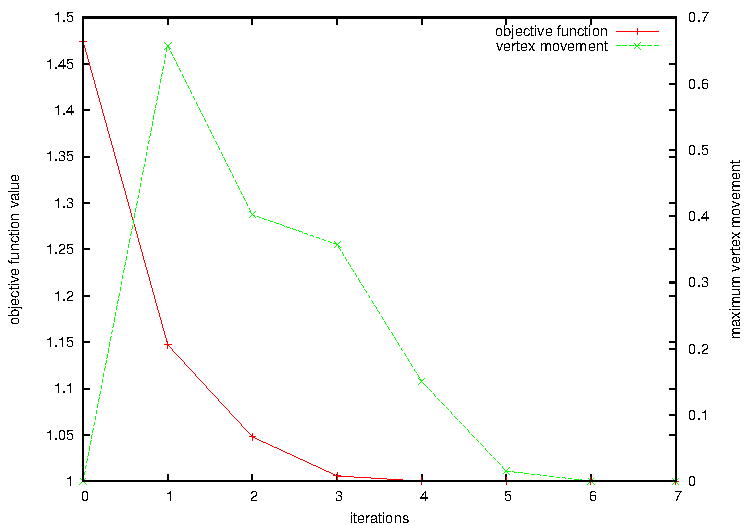
\includegraphics[width=5in]{figures/iterplot}
\caption{\em Convergence Plot \label{fig:iterplot}}
\end{center}
\end{figure}

\section{Viewing Meshes}

VTK files read and written by the {\texttt MeshImpl} class are viewable in a plethora of visualization tools that use the VTK visualization library.

The {\texttt Mesquite::MeshWriter} namespace contains functions to export mesh in a variety of formats for visualization including:
\begin{itemize}
\item GNU Plot
\item Visualization TookKit (VTK)
\item Encapsulated PostScript (EPS)
\item Scalable Vector Graphics (SVG)
\item StereoLithography (STL)
\end{itemize}
The GNU plot format writes line data that can be used to plot a wireframe of the mesh (the mesh edges).	 Both 2D and 3D meshes can be exported in this format.	A mesh can be plotted as a 2D projection with the GNU plot command:
\begin{verbatim}
plot 'filename' with linespoints
\end{verbatim}
or as a rotatable 3D plot with the command:
\begin{verbatim}
splot 'filename' with linespoints
\end{verbatim}
Figure \ref{fig:meshgpt} is the result of plotting the mesh contained in {\texttt testSuite/higher\_order/homogeneousPart.vtk} with GNU plot.

\begin{figure}[htb!]
\begin{center}
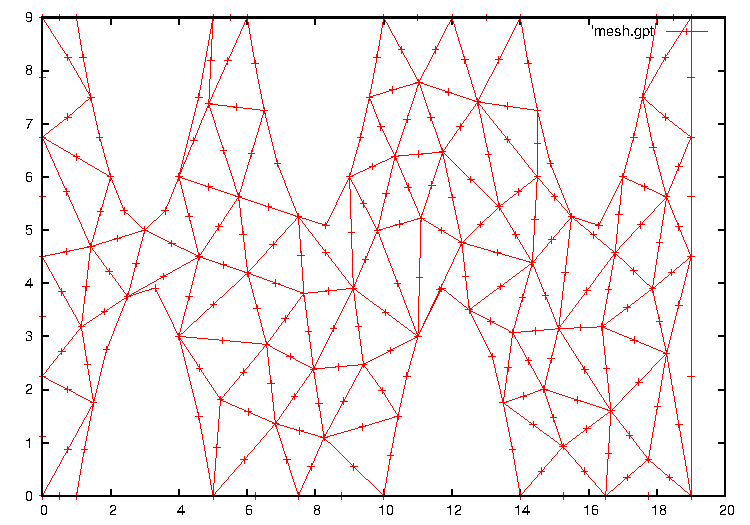
\includegraphics[width=4in]{figures/mesh_gpt}
\caption{\em GNU Plot of 2D Quadratic Triangles \label{fig:meshgpt}}
\end{center}
\end{figure}

As mentioned in the previous section, the VTK file format can be used with a variety of visualization tools.  Figure \ref{fig:meshvtk} shows a simple plot of the same mesh in the Paraview visualization tool.

\begin{figure}[htb!]
\begin{center}

\includegraphics[width=4in]{figures/mesh_vtk}
\caption{\em Paraview plot of 2D Quadratic Triangles \label{fig:meshvtk}}
\end{center}
\end{figure}

Figure \ref{fig:mesh} shows the output of the encapsulated PostScript writer for the mesh.  The EPS writer can write only 2D projections of the mesh.  The caller must specify a projection when calling {\texttt MeshWriter::write\_eps}.  The {\texttt testSuite/higher\_order/homogeneousPart.vtk} file contains quadratic triangle elements.  Compare the mesh edges on the mesh boundary in this plot with the output in Figures \ref{fig:meshgpt} and \ref{fig:meshvtk}.	The EPS writer in Mesquite exports the quadratic edges as curves corresponding to the classic quadratic edge shape function:
\begin{displaymath}
E(u) = \frac{1}{2}u(u-1)V_1 + (1-u^2)V_2 + \frac{1}{2}u(u+1)V_3
\end{displaymath}

\begin{figure}[htb!]
\begin{center}
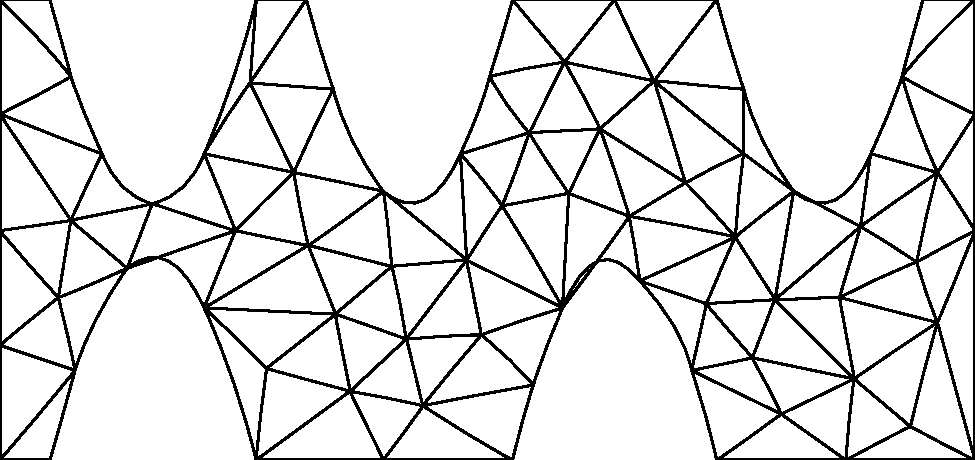
\includegraphics[width=4in]{figures/mesh}
\caption{\em Encapsulated PostScript of 2D Quadratic Triangles \label{fig:mesh}}
\end{center}
\end{figure}

The STL file format can be used to write only linear triangles.	 Higher-order triangular elements will be written as linear triangles.	An error will be returned if the mesh contains other element types.

\section{Exporting Mesh Quality}

The {\texttt QualityAssessor} class has the ability to store mesh quality values and other characteristics as tag data on mesh elements.  This data can be accessed directly by applications or written to a VTK file using the {\texttt MeshImpl} class or the applications native mesh writer (if it is capable of writing tag data.)	 The example code below was used to create the VTK file from which the Paraview plot in Figure \ref{fig:meshqual} was generated.

\begin{figure}[htb!]
\begin{center}
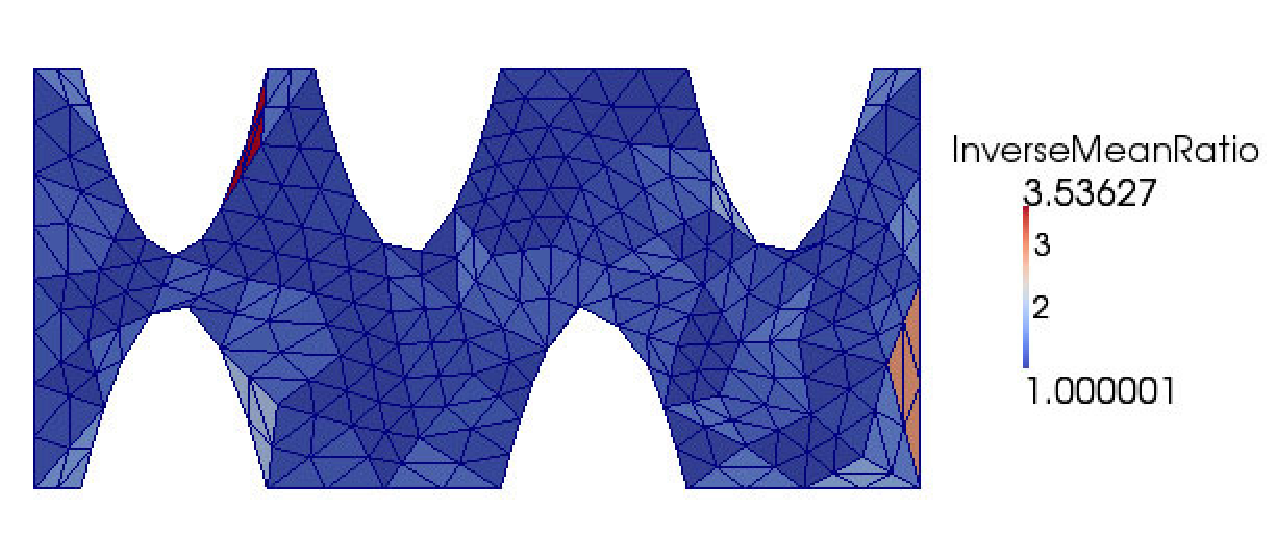
\includegraphics[width=5in]{figures/meshqual}
\caption{\em Paraview Plot Coloring Elements by Quality Metric Value \label{fig:meshqual}}
\end{center}
\end{figure}

\newpage
\begin{samepage}
\begin{lstlisting}[frame=single]
MsqError err;
MeshImpl mesh;
mesh.read_vtk( "homogeneousPart.vtk", err );

IdealWeightInverseMeanRatio metric;
QualityAssessor qa;
qa.add_quality_assessment(&metric,0,0,0,\<"InverseMeanRatio"\>);

PlanarDomain plane(PlanarDomain::XY);
InstructionQueue queue;
queue.add_quality_assessor( &qa, err );
MeshDomainAssoc mesh_and_domain = MeshDomainAssoc(&mesh, &plane);
queue.run_instructions( &mesh_and_domain, err );

mesh.write_vtk( "meshqual.vtk", err );
\end{lstlisting}
\end{samepage}

\begin{figure}[htb!]
\begin{center}
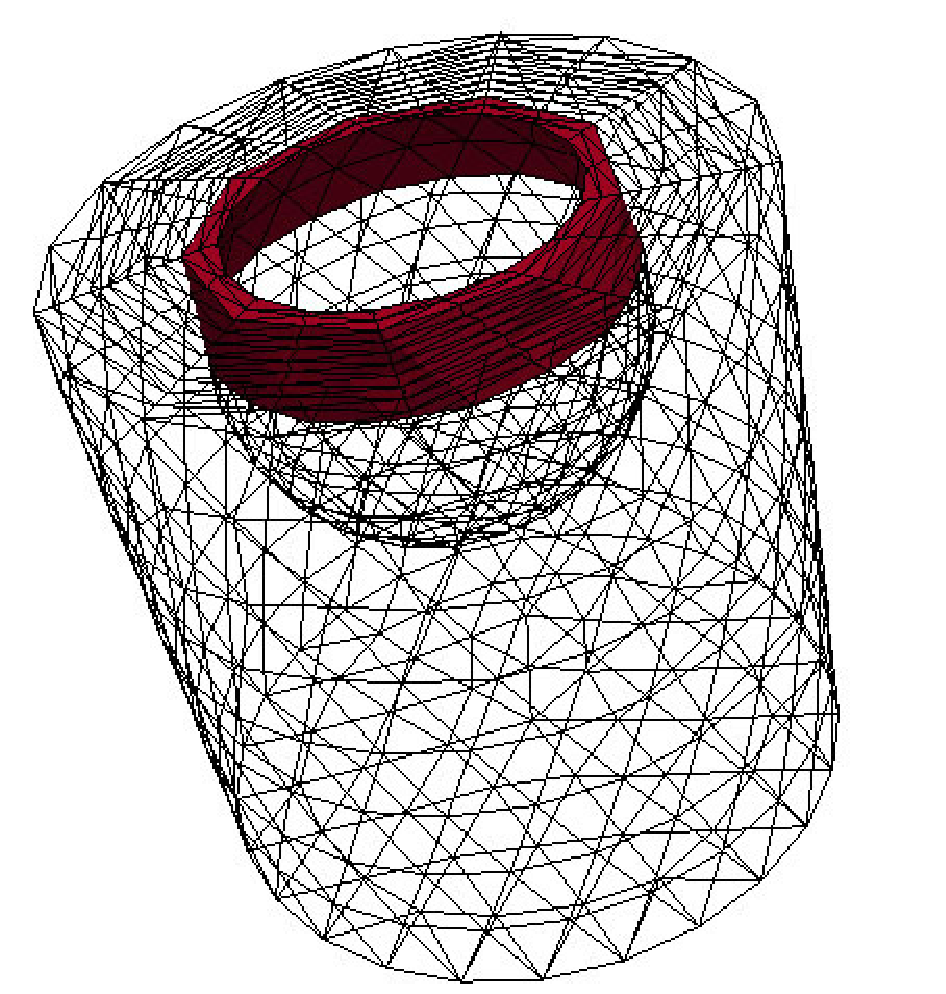
\includegraphics[width=3in]{figures/meshqual3d}
\caption{\em Paraview Plot Showing Inverted Elements \label{fig:meshqual3d}}
\end{center}
\end{figure}

Figure \ref{fig:meshqual3d} is a Paraview plot showing the inverted elements in a quadratic tetrahedral mesh.  The mesh is plotted twice: once as a simple wireframe of the mesh boundary and a second time as solid mesh with a threshold filter on the inverted flag exported by Mesquite.  The listing below shows how the {\texttt QualityAssessor} class can be instructed to flag inverted elements:

\newpage
\begin{lstlisting}[frame=single]
MsqError err;
MeshImpl mesh;
mesh.read_vtk( "sphereCylinder_1194_inv.vtk", err );

QualityAssessor qa;
\<qa.tag_inverted_elements("Inverted");\>

InstructionQueue queue;
queue.add_quality_assessor( &qa, err );
MeshDomainAssoc mesh_and_domain = MeshDomainAssoc(&mesh, &plane);
queue.run_instructions( &mesh_and_domain, err );

mesh.write_vtk( "meshqual.vtk", err );
\end{lstlisting}


\section{Mesh Optimization Visualization}

The Mesquite {\texttt TerminationCriterion} class can write the complete mesh after each iteration as either VTK or GNU Plot data suitable for viewing as an animation.	 Similar to requesting plot data as described in Section \ref {sec:optplot}, it is important to request this feature from the appropriate termination criterion instance.  If doing a global optimization, the feature should be activated for the {\em inner} termination criterion.  Otherwise the feature should almost always be activated for the {\em outer} termination criterion.

The command to request an animation of the mesh optimization in the VTK format is:
\begin{lstlisting}
tc.write_mesh_steps( "anim", TerminationCriterion::VTK );
\end{lstlisting}
This will produce a sequence of files named ``anim.1.vtk'', ``anim.2.vtk'', etc.  The files can be opened in visualization tools such as Paraview as a single set and played back as an animation.  If the optimization calculates the gradient of the objective function, that data will also be included in the file as vector data on each mesh vertex.  The components of the vector on each vertex are the partial derivatives of the objective function with respect to each coordinate value of the vertex.  A Paraview ``glyph'' filter can be used to display these vector values during the animation.


The command to request an animation of the mesh optimization in a format suitable for animating in GNU plot is:
\begin{lstlisting}
tc.write_mesh_steps( "anim", TerminationCriterion::GNUPLOT );
\end{lstlisting}
This will produce a sequence of files named ``anim.1'', ``anim.2'', etc.  It will also export a file named ``anim'' that contains the necessary GNU Plot commands to display the animation.




% Parallel Mesquite
\chapter{Using Mesquite in Parallel}
\label{sec:parallel}

\section{Introduction}

Large meshes are often partitioned across many parallel processors either because they are too large to fit into the memory of a single machine or in order to speed up the computation. Even if it would be possible to assemble all partitions on a single processor, smooth the mesh, and repartition the result, such an approach would be very I/O inefficient. Moreover, for larger meshes such an approach would quickly run out of memory and fail. Therefore Mesquite supports smoothing meshes in parallel.

Mesquite currently does only synchronous Nash-game or local optimizations in parallel \cite{Fr95}.  It does not yet provide parallel solvers and therefore cannot do either block coordinate descent or truly global optimizations in parallel (minimization of an explicit, global objective function.)

For algorithms such as Laplacian smoothing that are local optimizations, optimization in parallel is essentially the same as in serial.  For other optimizations that do a global minimization of an explicitly defined objective function in serial (for example \texttt{ShapeImprover}), the parallel optimization will be a Nash-game type optimization where the interior vertices (those not on the partition boundaries) will be optimized as a group.  Each vertex on the partition boundary will then be optimized individually.  While a global optimization in serial will typically have only one outer iteration, it is generally desirable to do multiple outer iterations in parallel so the Nash-game type optimization can reach convergence.  Mesquite wrappers (see Chapter \ref{sec:wrappers}) that implement global optimizations in serial default to 10 outer iterations in parallel.


\section{Distributed Mesh}

The input mesh for use in parallel quality improvement must be partitioned based on vertices.  That is, each vertex in the mesh must be assigned a single processor as its owner.  For optimal performance, vertices should be evenly distributed amongst available processors and the vertices assigned to the same processor should compose a contiguously connected patch of mesh.

Each processor must also have access to all elements for which the position of its vertices influence the quality.  For almost all algorithms in Mesquite, this is the set of all elements that contain one of the vertices.  Further, each processor must also be able to access any additional vertices owned by other processors that are necessary to define those elements.  The instances of such vertices on processors that do not own them are typically referred to as ``ghosted'' vertices.  Elements for which copies exist on multiple processors may sometimes also be referred to as ``ghosted'' or ``ghost'' elements.

\begin{figure*}[htbp]
\begin{center}
    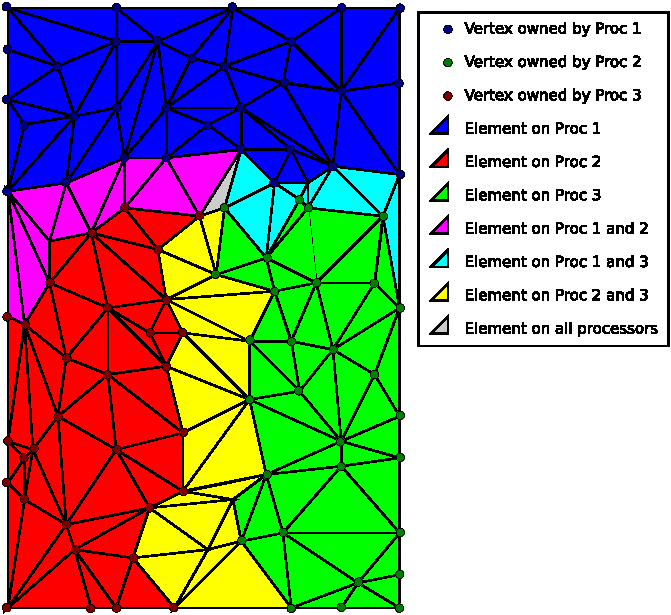
\includegraphics{figures/parallel_mesh}
    \caption{Sharing or ghosting of elements and vertices in a partitioned mesh.}
    \label{fig:parallel_mesh}
\end{center}
\end{figure*}

Figure \ref{fig:parallel_mesh} shows a mesh partitioned amongst three processors.  The vertices owned by the three different processors are shown in three different colors: blue, red, and green.  Elements are colored according to the processors for which copies of that element must be available.  A copy of an element must be available on each processor owning at least one of the vertices of the element.  Elements colored blue, red, or green need be visible only on the processor owning vertices of the corresponding color. The single grey element must have copies defined on all three processors because each of its vertices is owned by a different processor.  The remaining elements must be defined on at least two processors.

For a copy of an element to be available on a processor, all of its vertices must also be available on that processor.  So for all elements for which copies exist on more than one processor, the vertices contained in those elements must also exist as ghost vertices on at least one processor.  That is, copies of such vertices must exist on processors other than those that are responsible for optimizing the location of that vertex.  For example, copies of the yellow elements in Figure \ref{fig:parallel_mesh} exist on both the blue and the green processors.  All blue vertices in at least one yellow element must exist as ghost vertices on the green processor and all green vertices in at least one yellow element exist as ghost copies on the blue processor.  A copy of the grey element must exist on every processor.  Therefore each vertex in that element exist as ghost copies on both of the other two processors that do not own it.


\section{Input Data}

Assuming the mesh exists in partitioned form the user has to provide Mesquite with three things:
\begin{itemize}
\item a processor ID of type \texttt{int} for every vertex that determines which processor owns a vertex and is in charge for smoothing this vertex,
\item a global ID of type \texttt{size\_t} for every vertex that (at least in combination with the processor ID) is globally unique,
\item all necessary ghost elements and ghost nodes along the partition boundary must be provided.
\end{itemize}

The following copies of elements and vertices must exist: Elements must exist on all processors that own one or more of the vertices they reference. Vertices must exist on all processors that have some element referencing them.

The \texttt{Mesquite::ParallelMesh} class (\texttt{ParallelMeshInterface.hpp}) inherits \texttt{Mesquite::Mesh} and defines the interface Mesquite uses to interact with parallel mesh data. It contains the following additional pure virtual (or abstract) functions:
\begin{itemize}
\item get processor ids for given vertices,
\item get global ids for given vertices,
\item set and get a pointer to a \texttt{Mesquite::ParallelHelper} object.
\end{itemize}

To allow Mesquite direct access to the way you store the parallel mesh data you must inherit \texttt{Mesquite::ParallelMesh} and also implement your own get processor ID and get global ID functionality. The \texttt{Mesquite::ParallelHelper} class takes care of all the underlying communication using MPI. You will always use the \texttt{Mesquite::ParallelHelperImpl} implementation that we provide.

Alternatively you can turn any existing mesh of type \texttt{Mesquite::Mesh} into a parallel mesh of type\vspace{-5pt} \begin{center}
\texttt{Mesquite::ParallelMesh} by using the \texttt{Mesquite::ParallelMeshImpl}
\end{center} \vspace{-5 pt}implementation we provide. On creation it needs a pointer to an object of type \texttt{Mesquite::Mesh} and the names of two tags. It is expected that every vertex is properly tagged with the processor ID tag being of type INT and the global ID tag being of type HANDLE.


\subsection{ParallelMesh Implementation Requirements}
%%(this text needs to be added where GLOBAL_ID etc is discussed)

In addition to global and processor ID's, a tag named \texttt{LOCAL\_ID}, with type \texttt{INT}, must be provided in
your ParallelMesh implementation.  In summary, here are the tags and
their types required by Parallel Mesquite:

\begin{tabular}{ | l | l | l | }
  \hline
  Concept name & Typical/required code string &  Mesquite type \\
\hline
 vertex processor owner id & \texttt{PROCESSOR\_ID} (typical, implementation-dependent) & INT \\
 vertex global unique id & \texttt{GLOBAL\_ID} (typical,  implementation-dependent) & HANDLE \\
 vertex local id (internal use) & \texttt{LOCAL\_ID} (required) & INT \\
  \hline
\end{tabular}

If you obtained Mesquite from the Trilinos site, you can see a sample
imlementation of ParallelMesh in the stk\_percept package, at

\texttt{Trilinos/packages/stk/stk\_percept/stk\_percept/mesh/mod/mesquite-interface/PerceptMesquiteMesh.*pp.}

\section{ITAPS iMeshP Interface}

The MsqIMeshP class is an alternate implementation of the \texttt{ParallelMesh} interface that can be used to provide Mesquite with callbacks to access mesh and related parallel properties.  The ITAPS Working Group has defined a standard API for exchange of parallel mesh data between applications. The \texttt{Mesquite::MsqIMeshP} class declared in \texttt{MsqIMeshP.hpp} is an ``adaptor'':  it presents the iMeshP interface as the \texttt{Mesquite::ParallelMesh} interface.

This class will use the iMeshP API to query processor identifiers and global identifiers for mesh vertices.  However, the MPI-based communication routines implemented in \texttt{ParallelHelperImpl} are used rather to communicate updated vertex locations between processors, rather than the mechanism provided by the iMeshP implementation.

\section{Examples}

This section contains two different examples of simple stand-alone applications that demonstrate the use of the \texttt{LaplaceWrapper} smoother in parallel.  Both examples, in being stand-alone programs, load the mesh from one or more files.  When integrating Mesquite into an existing application where it is desired that Mesquite access application mesh data in memory, the initial setup will be different.  It will typically involve either providing some application-specific implementation of the \texttt{Mesh} and possibly \texttt{ParallelMesh} interfaces or instances of an appliction-specific \texttt{iMeshP} and \texttt{iMesh} implementation.

\subsection{Example: Parallel Laplacian Smooth}
\label{sec:parallel-example-1}

This example uses the \texttt{LaplaceWrapper} wrapper in parallel using the built-in \texttt{Mesh}, \texttt{ParallelMesh}, and \texttt{ParallelHelperImpl} implementations.  For this example to work, the mesh must be partitioned such that the mesh for each processor is saved in a separate file named \texttt{part-\%d.vtk}, with the \texttt{\%d} replaced with the processor rank.  Each VTK file must contain vertex attributes named \texttt{GID} and \texttt{PID} containing the global ID and owning processor rank for each vertex.  Further, as this example provides no geometric domain definition, the vertices on the boundary of the mesh must be designated as ``fixed'' for the problem setup to be valid.


\begin{verbatim}
/* Mesquite includes */
#include <Mesquite.hpp>
#include <MeshImpl.hpp>
#include <ParallelMeshImpl.hpp>
#include <ParallelHelper.hpp>
#include <MsqError.hpp>
#include <LaplaceWrapper.hpp>

/* other includes */
#include <mpi.h>
#include <iostream>
using namespace std;

int main( int argc, char* argv[] )
{
  /* init MPI */
  int rank, nprocs;
  if (MPI_SUCCESS != MPI_Init(&argc, &argv)) {
    cerr << "MPI_Init failed." << endl;
    return 2;
  }
  MPI_Comm_rank(MPI_COMM_WORLD, &rank);
  MPI_Comm_size(MPI_COMM_WORLD, &nprocs);

  /* create processor-specific file names */
  ostringstream in_name, out_name;
  in_name << "part-" << rank << ".vtk";
  out_name << "part-" << rank << "-smoothed.vtk";

  /* load different mesh files on each processor */
  Mesquite::MsqError err;
  Mesquite::MeshImpl mesh;
  mesh.read_vtk(in_name.str().c_str(), err);
  if (err) {cerr << err << endl; return 1;}

  /* create parallel mesh instance, specifying tags
   * containing parallel data */
  Mesquite::ParallelMeshImpl parallel_mesh(&mesh, "GID", "PID");
  Mesquite::ParallelHelperImpl helper;
  helper.set_communicator(MPI_COMM_WORLD);
  helper.set_parallel_mesh(&parallel_mesh);
  parallel_mesh.set_parallel_helper(&helper);

  /* do Laplacian smooth */
  LaplaceWrapper optimizer;
  optimizer.run_instructions(&parallel_mesh, err);
  if (err) {cerr << err << endl; return 1; }

  /* write mesh */
  mesh.write_vtk(out_name.str().c_str(),err);
  if (err) {cerr << err << endl; return 1;}

  MPI_Finalize();
  return 0;
}
\end{verbatim}

\subsubsection{Implementation of Example \ref{sec:parallel-example-1} }

In your Mesquite distribution, there is an implementation of the
example code for Lapalace smoothing in parallel, in the file
\texttt{mesquite/testSuite/parallel\_smooth\_laplace/par\_hex\_smooth\_laplace.cpp}.
This code reads in a serial or parallel-split set of VTK files and
smooths the mesh, then compares the result to a "gold" copy, which is
useful for regression testing (see \ref{sec:RegressionTesting}).

\subsubsection{Parallel Regression Tests}

In addition to the Laplace example, see \\
\texttt{mesquite/testSuite/parallel\_untangle\_shape/par\_hex\_untangle\_shape.cpp} \\
for example use of parallel mesh untangling and shape improvement, and
the associated files that begin with "par\_*" under the
\texttt{meshFiles/{2D,3D}/vtk/} directories.

For example, an initial, tangled quadrilateral mesh is shown in
\ref{fig:par_quad_orig}
while the result of untangling and smoothing is shown in
\ref{fig:par_quad_smoothed}.  A similar example with hexahedra is
shown in figures
\ref{fig:par_hex_orig}  and \ref{fig:par_hex_smoothed}.

\begin{figure*}[htpb]
\begin{center}
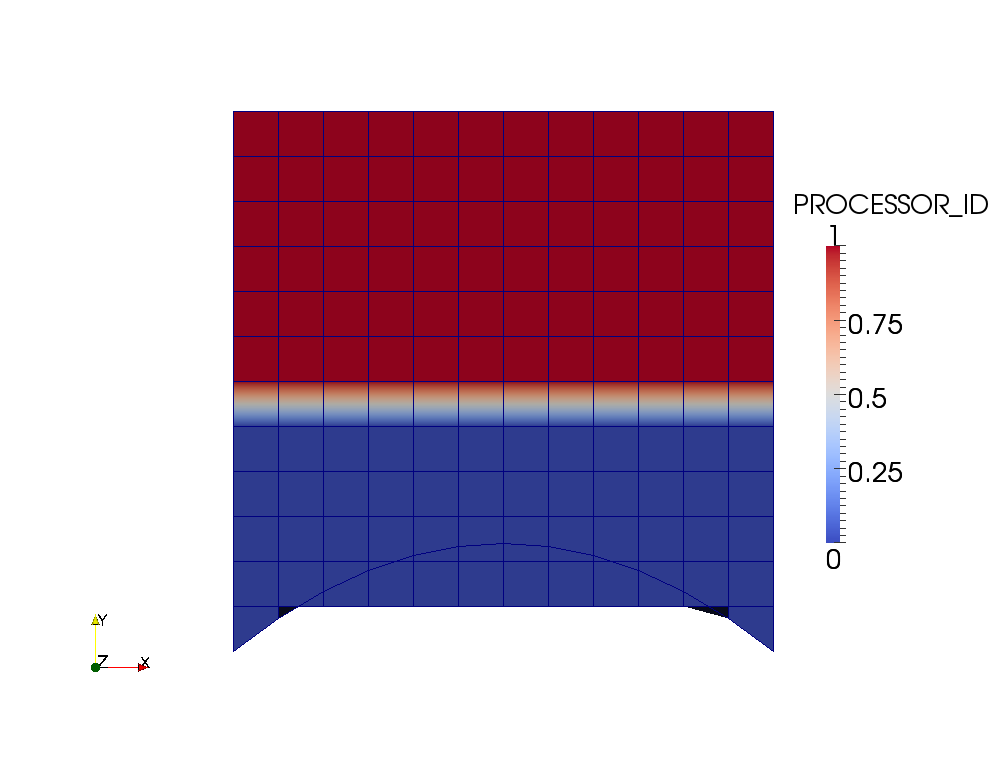
\includegraphics[width=4in]{figures/par-quad-orig}
\caption{Initial, tangled quadrilateral mesh.}
\label{fig:par_quad_orig}
\end{center}
\end{figure*}

\begin{figure*}[htpb]
\begin{center}
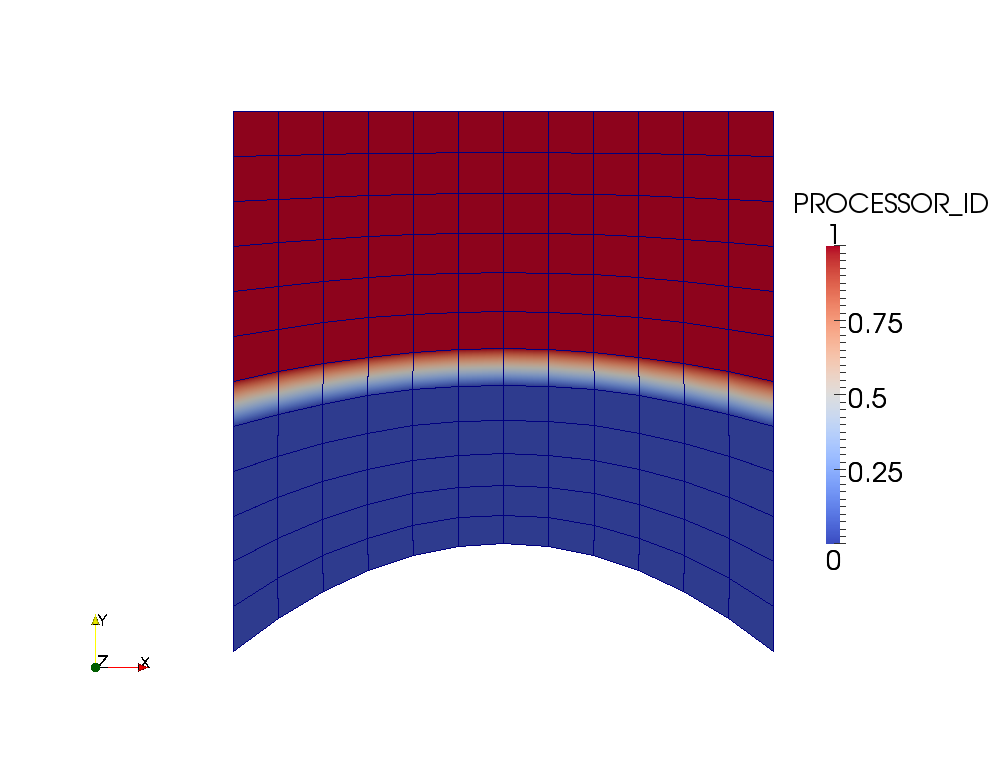
\includegraphics[width=4in]{figures/par-quad-smoothed}
\caption{Untangled and smoothed quadrilateral mesh.}
\label{fig:par_quad_smoothed}
\end{center}
\end{figure*}

\begin{figure*}[htpb]
\begin{center}
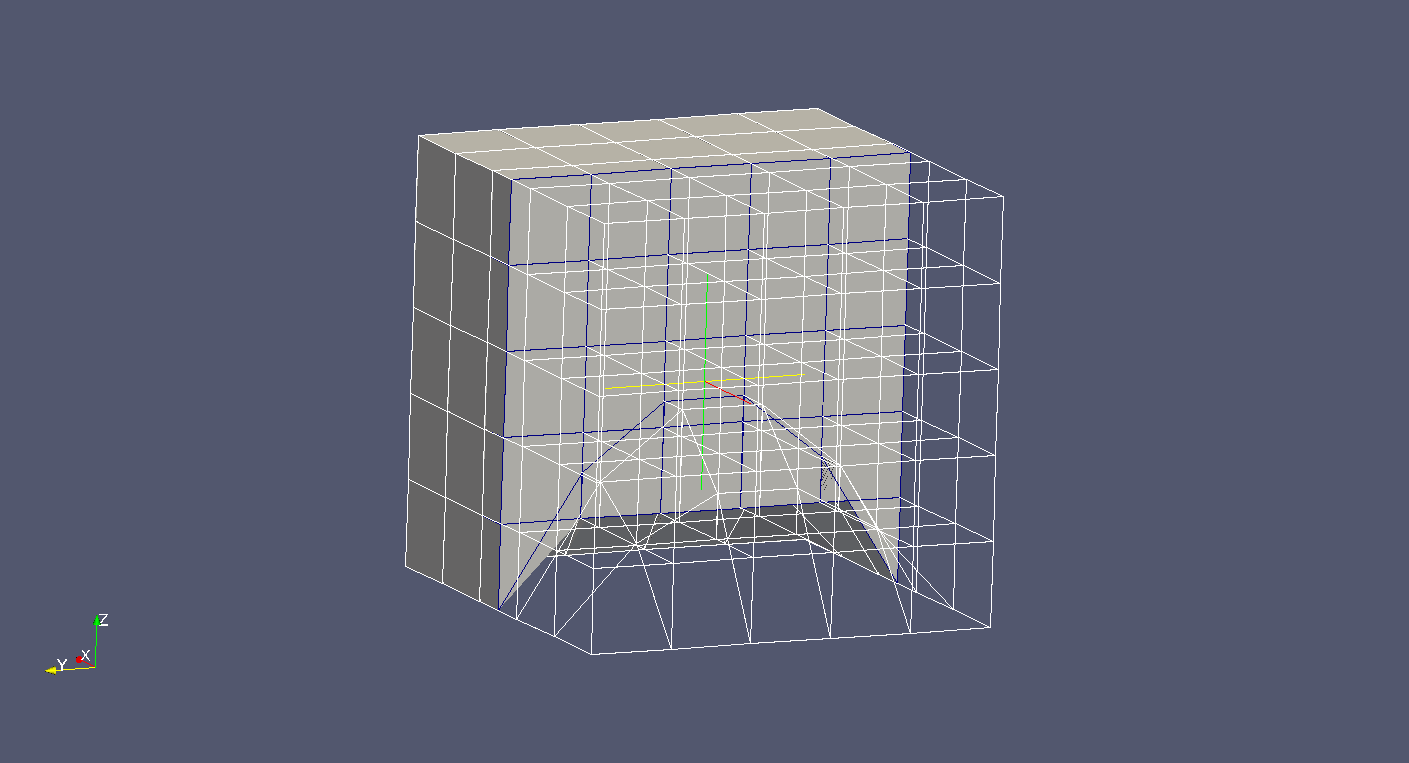
\includegraphics[width=4in]{figures/par-hex-orig}
\caption{Initial, tangled hexahedra mesh.}
\label{fig:par_hex_orig}
\end{center}
\end{figure*}

\begin{figure*}[htpb]
\begin{center}
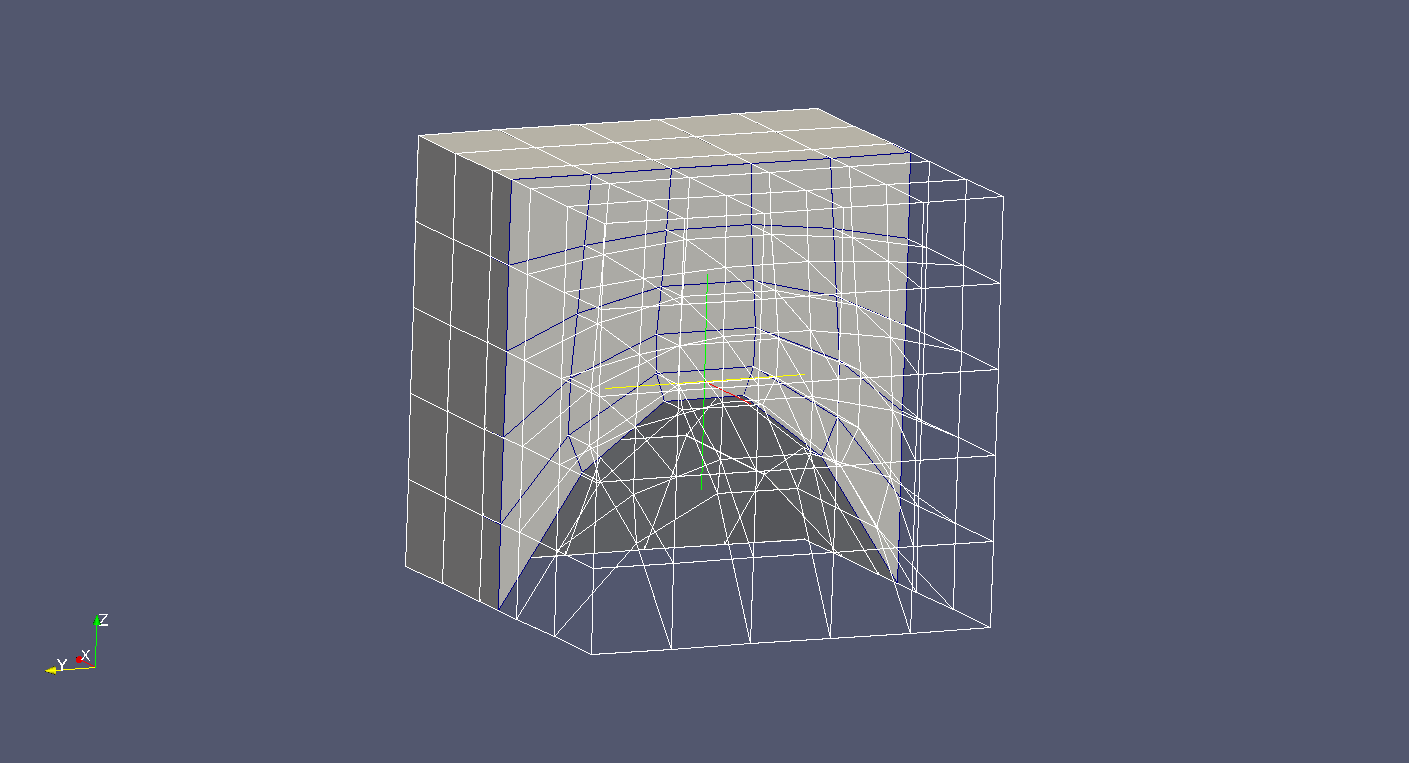
\includegraphics[width=4in]{figures/par-hex-smoothed}
\caption{Untangled and smoothed hexahedral mesh.}
\label{fig:par_hex_smoothed}
\end{center}
\end{figure*}

\subsection{Example: Using \texttt{Mesquite::Mesquite::MsqIMeshP}}

Similar to the example in Section \ref{sec:parallel-example-1}, this example uses the \texttt{LaplaceWrapper} wrapper in parallel to improve element shape.  However, this example assumes that either the iMeshP implementation is partitioning or that it is reading some pre-defined partitioned mesh and it relies on the iMeshP implementation to create ghost elements, assign global vertex IDs, etc.

An implementation of the iMesh and iMeshP APIs must be provided for this example to work.  Mesquite can use these APIs, but does not provide them.

\begin{verbatim}
/* Mesquite includes */
#include <Mesquite.hpp>
#include <MsqIMeshP.hpp>
#include <ParallelMeshImpl.hpp>
#include <ParallelHelper.hpp>
#include <MsqError.hpp>
#include <LaplaceWrapper.hpp>

/* other includes */
#include <mpi.h>
#include <iostream>
using namespace std;

int main( int argc, char* argv[] )
{
  const char input_file[] = "testmesh";
  const char output_file[] = "smoothmesh";

  /* init MPI */
  int rank, nprocs;
  if (MPI_SUCCESS != MPI_Init(&argc, &argv)) {
    cerr << "MPI_Init failed." << endl;
    return 2;
  }
  MPI_Comm_rank(MPI_COMM_WORLD, &rank);
  MPI_Comm_size(MPI_COMM_WORLD, &nprocs);

  /* create a new instance of the iMesh database */
  int ierr;
  iMesh_Instance mesh;
  iMesh_newMesh(NULL, &mesh, &ierr, 0);
  if (iBase_SUCCESS != ierr) return ierr;
  iBase_EntitySetHandle root_set;
  iMesh_getRootSet(mesh, &root_set, &ierr);
  if (iBase_SUCCESS != ierr) return ierr;

  /* create a partition instance in which to read
     the partitioned mesh */
  iMeshP_PartitionHandle partition;
  iMeshP_createPartitionAll(mesh, MPI_COMM_WORLD,
                            &partition, &err);
  if (iBase_SUCCESS != ierr) return ierr;

  /* load mesh */
  iMeshP_loadAll(mesh, partition, root_set, input_file,
                 NULL, &err, strlen(input_file), 0);
  if (iBase_SUCCESS != ierr) return ierr;

  /* create 1 layer of ghost entities */
  iMeshP_createGhostEntsAll(mesh, partition, 3, 1, 1, 0, &err);
  if (iBase_SUCCESS != ierr) return ierr;

  /* create MsqIMeshP instance */
  Mesquite::MsqError err;
  Mesquite::MsqIMeshP parallel_mesh(mesh, partition, root_set,
                                    iBase_REGION, err);
  if (err) {cerr << err << endl; return 1; }

  /* do Laplacian smooth */
  LaplaceWrapper optimizer;
  optimizer.run_instructions(&parallel_mesh, err);
  if (err) {cerr << err << endl; return 1; }

  /* write mesh */
  iMeshP_saveAll(mesh, partition, root_set, output_file,
                 NULL, &ierr, strlen(output_file), 0);
  if (iBase_SUCCESS != ierr) return ierr;

  /* cleanup */
  iMeshP_destroyPartitionAll(mesh, partition, &ierr);
  if (iBase_SUCCESS != ierr) return ierr;
  iMesh_dtor(mesh, &ierr);
  if (iBase_SUCCESS != ierr) return ierr;
  MPI_Finalize();
  return 0;
}
\end{verbatim}


%\input{api.tex}

%\input{extend.tex}

%\input{trouble.tex}

%\input{caveats.tex}

\input{support.tex}

\appendix

\input{team.tex}

\input{ack.tex}


\bibliographystyle{plain}
\bibliography{mesquite}


\end{document}


